%% (Master) Thesis template
%% Template version used: v1.4 (CADMO, ETHZ)
%%
%% Largely adapted from Adrian Nievergelt's template for the ADPS
%% (lecture notes) project.

%%%%%%%%%%%%%%%%%%%%%%%%%%%%%%%%%%%%%%%%%%%%%%%%%%%%%%%%%%%%%%%%%%%%%%%%%%%%%%%
%%%  Document settings                                                      %%%
%%%%%%%%%%%%%%%%%%%%%%%%%%%%%%%%%%%%%%%%%%%%%%%%%%%%%%%%%%%%%%%%%%%%%%%%%%%%%%%

%% We use the memoir class because it offers a many easy to use features.
\documentclass[9pt,b5paper,titlepage]{memoir}
\renewcommand{\baselinestretch}{1.1}
\usepackage{morewrites}

%% LaTeX Font encoding -- DO NOT CHANGE
\usepackage[T1]{fontenc}

%% Babel provides support for languages.  'english' uses British
%% English hyphenation and text snippets like "Figure" and
%% "Theorem". Use the option 'ngerman' if your document is in German.
%% Use 'american' for American English.  Note that if you change this,
%% the next LaTeX run may show spurious errors.  Simply run it again.
%% If they persist, remove the .aux file and try again.
\usepackage[english]{babel}

%% Input encoding 'utf8'. In some cases you might need 'utf8x' for
%% extra symbols. Not all editors, especially on Windows, are UTF-8
%% capable, so you may want to use 'latin1' instead.
\usepackage[utf8]{inputenc}

%% to allow cloring in code listings
\usepackage[dvipsnames]{xcolor}


%% This changes default fonts for both text and math mode to use Herman Zapfs
%% excellent Palatino font.  Do not change this.
\usepackage[sc]{mathpazo}

%% The AMS-LaTeX extensions for mathematical typesetting.  Do not
%% remove.
\usepackage{amsmath,amssymb,amsfonts,mathrsfs}

%% NTheorem is a reimplementation of the AMS Theorem package. This
%% will allow us to typeset theorems like examples, proofs and
%% similar.  Do not remove.
%% NOTE: Must be loaded AFTER amsmath, or the \qed placement will
%% break
\usepackage[amsmath,thmmarks]{ntheorem}
%% alog align groups to be split over pages
\allowdisplaybreaks

%% LaTeX' own graphics handling
\usepackage{graphicx}

%% This allows you to add .pdf files. It is used to add the
%% declaration of originality.
\usepackage{pdfpages}

%% Some more packages that you may want to use.  Have a look at the
%% file, and consult the package docs for each.
%% See the TeXed file for more explanations

%% [OPT] Multi-rowed cells in tabulars
\usepackage{multirow}

%% [REC] Intelligent cross reference package. This allows for nice
%% combined references that include the reference and a hint to where
%% to look for it.
\usepackage{varioref}

%% [OPT] Easily changeable quotes with \enquote{Text}
\usepackage[german=swiss]{csquotes}

%% [REC] Format dates and time depending on locale
\usepackage{datetime}

%% [OPT] Provides a \cancel{} command to stroke through mathematics.
%\usepackage{cancel}

%% [NEED] This allows for additional typesetting tools in mathmode.
%% See its excellent documentation.
\usepackage{mathtools}

%% [ADV] Conditional commands
%\usepackage{ifthen}

%% [OPT] Manual large braces or other delimiters.
%\usepackage{bigdelim, bigstrut}

%% [REC] Alternate vector arrows. Use the command \vv{} to get scaled
%% vector arrows.
\usepackage[h]{esvect}

%% [NEED] Some extensions to tabulars and array environments.
\usepackage{array}

%% [OPT] Postscript support via pstricks graphics package. Very
%% diverse applications.
%\usepackage{pstricks,pst-all}

%% [?] This seems to allow us to define some additional counters.
%\usepackage{etex}

%% [ADV] XY-Pic to typeset some matrix-style graphics
%\usepackage[all]{xy}

%% [OPT] This is needed to generate an index at the end of the
%% document.
%\usepackage{makeidx}

%% [OPT] Fancy package for source code listings.  The template text
%% needs it for some LaTeX snippets; remove/adapt the \lstset when you
%% remove the template content.
\usepackage[outputdir=.build]{minted}
\usepackage[most]{tcolorbox}
\usepackage{float}
\usepackage{afterpage}

%% [REC] Fancy character protrusion.  Must be loaded after all fonts.
\usepackage[activate]{pdfcprot}

%% [REC] Nicer tables.  Read the excellent documentation.
\usepackage{booktabs}

%% bibliography related
\usepackage[natbib,
  authordate,
  backend=biber,
  isbn=false,
  numbermonth=false]{biblatex-chicago}
\addbibresource{mendeley.bib}
%% non-utf8 characters imported by mendeley into the bibliography
\DeclareUnicodeCharacter{2010}{-}
\DeclareUnicodeCharacter{0301}{/}
%% hide language field/url in certain types
\DeclareSourcemap{
  \maps{
    \map{
      \step[fieldset=language, null]
    }
    \map{
      \pertype{article}
      \pertype{book}
      \pertype{inbook}
      \step[fieldset=url, null]
    }
  }
}
% enable linebreaks after the doi keyword
\DeclareFieldFormat{doi}{%
  \textrm{doi}\addcolon\allowbreak
  \ifhyperref
    {\href{http://dx.doi.org/#1}{\nolinkurl{#1}}}
    {\nolinkurl{#1}}}
% settings for linebreak penalties in urls/dois
\setcounter{biburllcpenalty}{100}
\setcounter{biburlucpenalty}{200}
% remove dashes in repeat authors
\makeatletter
\AtEveryBibitem{%
  \global\undef\bbx@lasthash%
  \clearfield{extrayear}}
\makeatother
%% use same for for urls/dois
\urlstyle{same}

%% glossary/acronyms
\usepackage[nogroupskip, toc]{glossaries}
\usepackage{glossary-mcols}
\glsdisablehyper
\makeglossaries
\glsenableentrycount
\renewcommand*{\glspostdescription}{} % Removes dots at the end of each entry.

%% greek letters in text mode
\usepackage[euler]{textgreek}

%% checkmark and other symbols
%\usepackage{pifont}

%% rotate cells in tables
\usepackage[figuresright]{rotating}

%% for degree symbols and other unit stuffs
\usepackage[binary-units=true]{siunitx}

%% inline lists
\usepackage[inline]{enumitem}

%% stoichiometric formulae and chemical equations
\usepackage[version=4]{mhchem}

%% capability for multiple footnotes & footnotes in section headings
\usepackage[multiple, stable]{footmisc}

%% for indicator function 1
\usepackage{dsfont}
\usepackage{xparse}

%% Our layout configuration.  DO NOT CHANGE.
%% Memoir layout setup

%% NOTE: You are strongly advised not to change any of them unless you
%% know what you are doing.  These settings strongly interact in the
%% final look of the document.

%% Title page: redefine maketitle macro
\newlength{\logounitlength}
\setlength{\logounitlength}{0.08mm}

\def\thesistype#1{\def\thesistypestring{#1}}
\def\thesistypestring{}
\def\thesisperiod#1{\def\thesisperiodstring{#1}}
\def\thesisperiodstring{}
\def\thesistitle#1{\def\thesistitlestring{#1}}
\def\thesistitlestring{}
\def\thesisauthor#1{\def\thesisauthorstring{#1}}
\def\thesisauthorstring{}
\def\submissiondate#1{\def\submissiondatestring{#1}}
\def\submissiondatestring{}
\def\alternatereader#1{\def\alternatereaderstring{#1}}
\def\alternatereaderstring{}
\def\mainreader#1{\def\mainreaderstring{#1}}
\def\mainreaderstring{}

\newcommand{\ETHlogo}{
  \parbox{100mm}{
    \vbox{
      \kern2pt\setlength{\unitlength}{\logounitlength}
      \begin{picture}(330,110)(0,-5)
        \thicklines
        \multiput(0,0)(2,0){16}{\line(1,4){25}}
        \multiput(1,0)(0.5,2){12}{\line(1,0){84}}
        \multiput(42,40.4)(0.5,2){11}{\line(1,0){53}}
        \multiput(19.5,78.8)(0.5,2){12}{\line(1,0){210}}
        \multiput(116,0)(2,0){16}{\line(1,4){24}}
        \multiput(180,0)(2,0){16}{\line(1,4){25}}
        \multiput(237,0)(2,0){16}{\line(1,4){25}}
        \multiput(220,39)(0.5,2){12}{\line(1,0){30}}
        \put(262.5,100){\line(1,0){30}}
      \end{picture}
      \hfill\break\sffamily\bfseries Swiss Federal Institute of Technology 
      Zurich
    }
  }
}

\newcommand{\SfSlogo}{
  \parbox{40mm}{
    \hfill\kern2pt
    \setlength{\unitlength}{\logounitlength}\begin{picture}(330,110)(0,-5)
    \end{picture}\\
    \sffamily\bfseries
    \null\hfill Seminar for\kern3mm\break
    \null\hfill \phantom{g}Statistics\kern3mm%
  }
}

\makeatletter
\def\maketitle{
  \begingroup
  \hspace*{-3pt}\raise 20pt\hbox{\ETHlogo}\hfill
    \raise 19pt\hbox{\SfSlogo}\hspace*{-10pt}
  \linebreak
  \vspace{1pt}
  {\sffamily\bfseries\noindent{\\Departement of Mathematics}}
  \par\vspace*{5pt}
  \rule{\linewidth}{.3pt}\\[1pt]
  \vspace*{-15pt}
  \begin{center}
    \Large \thesistypestring
    \hfill
    \Large \thesisperiodstring\\[2pt] 
  \end{center}
  \rule{\linewidth}{.3pt}
  \medskip
  \vspace{70pt}
  \begin{center}
    \bfseries
    \Large \thesisauthorstring\\
    \vspace{2ex plus 1ex minus 1.5ex}
    \LARGE \thesistitlestring
  \end{center}
  \vspace{\stretch{2}}
  \vspace{\stretch{3}}

  \begin{center} \large
    \rule{.5\linewidth}{.3pt} \\[8pt]
    \begin{tabular}{ll}
      Submission Date: & \submissiondatestring
    \end{tabular}
    \\[5pt] \rule{.5\linewidth}{.3pt}
    
    \vspace{2ex plus 25ex minus 1.5ex}
    
    \begin{tabular}{ll}
      Co-Adviser: & \alternatereaderstring \\
      Adviser:    & \mainreaderstring
    \end{tabular}
  \end{center}
  \vspace*{-20pt}

  \endgroup
}
\makeatother

%% Turn extra space before chapter headings off.
\setlength{\beforechapskip}{0pt}

\nonzeroparskip
\parindent=0pt
\defaultlists

%% Chapter style redefinition
\makeatletter

\if@twoside
  \pagestyle{Ruled}
  \copypagestyle{chapter}{Ruled}
\else
  \pagestyle{ruled}
  \copypagestyle{chapter}{ruled}
\fi
\makeoddhead{chapter}{}{}{}
\makeevenhead{chapter}{}{}{}
\makeheadrule{chapter}{\textwidth}{0pt}
\copypagestyle{abstract}{empty}

\makechapterstyle{bianchimod}{%
  \chapterstyle{default}
  \renewcommand*{\chapnamefont}{\normalfont\Large\sffamily}
  \renewcommand*{\chapnumfont}{\normalfont\Large\sffamily}
  \renewcommand*{\printchaptername}{%
    \chapnamefont\centering\@chapapp}
  \renewcommand*{\printchapternum}{\chapnumfont {\thechapter}}
  \renewcommand*{\chaptitlefont}{\normalfont\huge\sffamily}
  \renewcommand*{\printchaptertitle}[1]{%
    \hrule\vskip\onelineskip \centering \chaptitlefont\textbf{\vphantom{gyM}##1}\par}
  \renewcommand*{\afterchaptertitle}{\vskip\onelineskip \hrule\vskip
    \afterchapskip}
  \renewcommand*{\printchapternonum}{%
    \vphantom{\chapnumfont {9}}\afterchapternum}}

%% Use the newly defined style
\chapterstyle{bianchimod}

\setsecheadstyle{\Large\bfseries\sffamily}
\setsubsecheadstyle{\large\bfseries\sffamily}
\setsubsubsecheadstyle{\bfseries\sffamily}
\setparaheadstyle{\normalsize\bfseries\sffamily}
\setsubparaheadstyle{\normalsize\itshape\sffamily}
\setsubparaindent{0pt}

%% Set captions to a more separated style for clearness
\captionnamefont{\sffamily\bfseries\footnotesize}
\captiontitlefont{\sffamily\footnotesize}
\setlength{\intextsep}{16pt}
\setlength{\belowcaptionskip}{1pt}

%% Set section and TOC numbering depth to subsection
\setsecnumdepth{subsection}
\settocdepth{subsection}

\checkandfixthelayout

\setlength{\droptitle}{-48pt}

\makeatother

%% This defines how theorems should look. Best leave as is.
\theoremstyle{plain}
\setlength\theorempostskipamount{0pt}


%% Theorem environments.  You will have to adapt this for a German
%% thesis.
\input{setup/theoremsetup}

%% Helpful macros.
%% Custom commands
%% ===============

%% Special characters for number sets, e.g. real or complex numbers.
\newcommand{\C}{\mathbb{C}}
\newcommand{\K}{\mathbb{K}}
\newcommand{\Nat}{\mathbb{N}}
\newcommand{\Q}{\mathbb{Q}}
\newcommand{\R}{\mathbb{R}}
\newcommand{\Z}{\mathbb{Z}}
\newcommand{\X}{\mathbb{X}}

%% Fixed/scaling delimiter examples (see mathtools documentation)
\DeclarePairedDelimiter\abs{\lvert}{\rvert}
\DeclarePairedDelimiter\norm{\lVert}{\rVert}

%% Use the alternative epsilon per default and define the old one as \oldepsilon
\let\oldepsilon\epsilon
\renewcommand{\epsilon}{\ensuremath\varepsilon}

%% Also set the alternate phi as default.
\let\oldphi\phi
\renewcommand{\phi}{\ensuremath{\varphi}}

\newcommand\given[1][]{\:#1\vert\:}
\let\existstemp\exists
\let\foralltemp\forall
\renewcommand{\exists}{\ensuremath\enskip\existstemp\:}
\renewcommand{\forall}{\ensuremath\enskip\foralltemp\:}

%% excerpts from SfS texab.sty
%% ===========================
%% R program
\newcommand*{\Rp}{\textsf{R}$\;$}
%% the epsfCfile function used in an example
\makeatletter
\newcommand{\@epsFFile}[2]{\includegraphics[#1]{#2}}
\newcommand{\epsFracFile}[2]{\@epsFFile{width=#1\textwidth}{#2}}%
\newcommand{\epsFracFileRot}[3][-90]{\@epsFFile{angle=#1,width=#2\textwidth}{#3}}
\newcommand{\epsfCfile}[2]{\centerline{\epsFracFile{#1}{#2}}}%
\newcommand{\epsfCfileRot}[3][-90]{\centerline{\epsFracFileRot[#1]{#2}{#3}}}%
\makeatother

\DeclareMathOperator{\logit}{logit}
\DeclareMathOperator{\med}{med}
\DeclareMathOperator{\median}{median}
\DeclareMathOperator{\Med}{Med}
\DeclareMathOperator{\Erw}{\mathbf{E}}%-- see also \E (below)
\DeclareMathOperator{\var}{var}
\DeclareMathOperator{\Var}{Var}
\DeclareMathOperator{\Cov}{Cov}
\DeclareMathOperator{\cov}{cov}
\DeclareMathOperator{\Cor}{Corr}
\DeclareMathOperator{\cor}{corr}
\DeclareMathOperator{\se}{se}
\DeclareMathOperator{\sd}{sd}
\DeclareMathOperator{\sign}{sign}
\DeclareMathOperator{\trace}{tr}
\DeclareMathOperator{\const}{const}
\DeclareMathOperator{\diag}{diag}
%% Nachteil von diesen (wegen \limits !?): \argmax_\beta setzt \beta
%% *unterhalb*, auch inline, was  \max_\beta nicht tut
%% \newcommand{\argmin}{\mathop{\arg \min}\limits}
%% \newcommand{\argmax}{\mathop{\arg \max}\limits}
%% \newcommand{\ave}{\mathop{ave}\limits}
%% This is following http://en.wikipedia.org/wiki/Arg_max 's recommendation:
\DeclareMathOperator*{\ave}{ave}
\DeclareMathOperator*{\argmin}{arg\, min}
\DeclareMathOperator*{\argmax}{arg\, max}
%
\DeclareMathOperator{\IF}{IF}
\DeclareMathOperator{\und}{ und }
\DeclareMathOperator{\oder}{ oder }
%\def\mit{\mathrm{ mit }}  %-- causes some problems with \mbox or \boldmath !!!
\DeclareMathOperator{\for}{ for }
\DeclareMathOperator{\where}{ where }
\DeclareMathOperator{\with}{ with }
%%-------  NB.  << NEVER >> REdefine  \or !!! ----
%% Not ``\and'': this is used in \author

% - Math. Operatoren
\newcommand{\op}[1]{\mathop{#1}}%was\newcommand{\op}[1]{\kern-.2em #1\kern-.2em}
% \newcommand{\oneover}[1]{{1\over#1}\,\,}
\newcommand{\oneover}[1]{{\textstyle 1\over#1}}
\newcommand{\inv}{^{-1}}
\newcommand{\sups}[1]{^{(#1)}}
%%-- shorter, for convergence ...==== unnecessary ===
%%-- There is already \to  (in standard TeX & LaTeX !) :
\newcommand{\go}{\rightarrow%
        \typeout{use standard \TeX \verb|\to| instead of \verb|\go|}}
%% convergence in Probability, Distribution: \tendsto{P}, \tendsto{D} :
\newcommand{\tendsto}[1]{\buildrel {#1} \over \longrightarrow}
\newcommand{\wt}{\widetilde}
\newcommand{\wh}[1]{\if \sigma{#1}\widehat{\sigma}\else
{}\kern0.1em\widehat{\kern-0.1em#1}{}\fi}
\newcommand{\wb}[1]{{}\if Y#1\overline{Y}\else
\kern0.2em\overline{\kern-0.2em#1}\fi}
\newcommand{\Ssum}{\sum\nolimits}
\newcommand{\Sn}{\Ssum_{i=1}^n}
\newcommand{\Seq}[4]{#1_{#2},\,#1_{#3},\ldots,#1_{#4}}% siehe auch \Nl , \No (unten)
\newcommand{\Half}{{\textstyle 1\over2}}% siehe auch \half (unten)
\newcommand{\ul}[1]{\textbf{#1}}

\newcommand{\Hmu}{\widehat{\mu}}
\newcommand{\Halpha}{\widehat{\alpha}}
\newcommand{\Hbeta}{\widehat{\beta}}
%
\newcommand{\iid}{\mbox{ i.i.d. }}
\newcommand{\fs}{\mbox{f.s.}}
\newcommand{\Loglik}{\ell\kern-1pt\ell}

%%%------------ script und andere Spezialschriften ----------------------


\DeclareMathOperator{\N}{\mathcal{N}}% Normalverteilung
\renewcommand{\P}{\mathcal{P}}%--- RE-defining the standard \P (Paragraph)!!--
%%%
\DeclareMathOperator{\M}{\mathcal{M}}% Multinom ?
\DeclareMathOperator{\B}{\mathcal{B}}% Binom
\DeclareMathOperator{\Bern}{\mathcal{B}ernoulli}
\DeclareMathOperator{\E}{\mathcal{E}}%-- see also \Erw (above)
\DeclareMathOperator{\F}{\mathcal{F}}
\DeclareMathOperator{\Wish}{\mathcal{W}}
\newcommand{\phibf}{\boldsymbol{\phi}}%{\phi\hskip-5.4pt\phi} % bold \phi


%% Make document internal hyperlinks wherever possible. (TOC, references)
%% This MUST be loaded after varioref, which is loaded in 'extrapackages'
%% above.  We just load it last to be safe.
\usepackage{hyperref}
\definecolor{hrlink}{rgb}{0.192, 0.494, 0.8}
\definecolor{hrcite}{rgb}{0.192, 0.494, 0.8}
\definecolor{hrurl}{rgb}{0.69, 0.353, 0.396}
\hypersetup{
  %hyperindex,
  colorlinks={true},
  %pagebackref,
  linktocpage,
  plainpages={false},
  linkcolor={hrlink},
  citecolor={hrlink},
  urlcolor={hrurl},
  pdfstartview={Fit},
  pdfview={XYZ null null null}
}


%% Set the paths where all figures are taken from:
\graphicspath{{figures/}}
%% level on which equation numbering is done
\numberwithin{equation}{chapter}
%% import knitr related stuff
\input{R/knitrPreamble}
\input{R/ggplotTheme}
%% glossary definitions
%% biology
\newacronym{ote}{OTE}{off-target effects}
\newacronym{hts}{HTS}{high throughput screening}
\newacronym{lof}{LOF}{loss-of-function}
\newacronym{hcs}{HCS}{high content screening}
% t3ss/t4ss
\newacronym{t3ss}{T3SS}{type III secretion system}
\newacronym{ipa}{Ipa}{\textit{Shigella} invasion protein}
\newacronym{sop}{Sop}{\textit{Salmonella} outer protein}
\newacronym{inv}{Inv}{\textit{Salmonella} invasion protein}
\newacronym{sptp}{SptP}{\textit{Salmonella} protein tyrosine phosphatase}
\newacronym{ssp}{Ssp}{\textit{Salmonella}-secreted protein}
\newacronym{ssa}{Ssa}{\textit{Sal\-mon\-ella} secretion system apparatus protein}
\newacronym{mxi}{Mxi}{\textit{Shigella} membrane expression of ipa}
\newacronym{pho}{Pho}{phosphate metabolism protein}
\newacronym[description={\textit{Salmonella} \acrshort{pho}[P]-repressed gene}]{prg}{Prg}{\textit{Salmonella} PhoP-repressed gene}
\newacronym{spa}{Spa}{\textit{Salmonella} surface presentation of antigen}
\newacronym{org}{Org}{\textit{Salmonella} oxygen-regulated gene}
\newacronym{sse}{Sse}{\textit{Salmonella} secreted effector protein}
\newacronym{sic}{Sic}{\textit{Salmonella} invasion chaperone protein}
\newacronym{ssc}{Ssc}{\textit{Salmonella} secreted chaperone protein}
\newacronym{ipg}{Ipg}{\textit{Shigella} invasion plasmid gene}
\newacronym{sif}{Sif}{\textit{Salmonella}-induced filament}
\newacronym{spv}{Spv}{\textit{Salmonella} plasmid virulence}
\newacronym{ics}{Ics}{\textit{Shigella} intracellular spread protein}
\newacronym{vir}{Vir}{virulence spread protein}
\newacronym{hil}{Hil}{\textit{Salmonella} hyperinvasion locus}
\newacronym{omp}{Omp}{\textit{Salmonella} outer-membrane protein}
\newacronym{avra}{AvrA}{\textit{Salmonella} avirulence protein A}
\newacronym{osp}{Osp}{outer \textit{Shigella} protein}
\newacronym{tir}{Tir}{translocated intimin receptor}
\newacronym{sip}{Sip}{\textit{Salmonella} invasion protein}
\newacronym{t4ss}{T4SS}{type IV secretion system}
% biochemistry
\newacronym{galnac}{GalNAc}{N-acetylgalactosamine}
\newacronym{gtp}{GTP}{guanosine triphosphate}
\newacronym{gdp}{GDP}{guanosine diphosphate}
\newacronym{gef}{GEF}{guanine nucleotide exchange factor}
\newacronym[description={\acrshort{gtp}ase activating protein}]{gap}{GAP}{GTPase activating protein}
\newacronym{rt}{RT}{reverse transcriptase}
\newacronym{ras}{Ras}{rat sarcoma family protein}
\newacronym[description={\acrshort{ras}-related nuclear protein}]{ran}{Ran}{Ras-related nuclear protein}
\newacronym[description={\acrshort{ras}-related in brain}]{rab}{Rab}{Ras-related in brain}
\newacronym[description={\acrshort{ras}-related C3 botulinum toxin substrate 1}]{rac-1}{Rac1}{Ras-related C3 botulinum toxin substrate 1}
\newacronym{arp23}{Arp2/3}{actin-related-protein 2 and 3}
\newacronym{cdc-42}{Cdc42}{cell division control protein 42 homolog}
\newacronym{vegf}{VEGF}{vascular endothelial growth factor}
\newacronym{icam-1}{ICAM-1}{intercellular adhesion mol\-ecule 1}
\newacronym{il-8}{IL-8}{interleukin-8}
\newacronym{lps}{LPS}{lipopolysaccharide}
\newacronym{tlr}{TLR}{toll-like receptor}
\newacronym{prpc}{PrPC}{cellular prion protein}
\newacronym{hsp}{HSP}{heat shock protein}
\newacronym{tir-1}{TIR}{toll-interleukin-1 receptor}
\newacronym{mhc}{MHC}{major histocompatibility complex}
\newacronym{cop-2}{COPII}{coat protein complex II}
\newacronym{tap}{TAP}{tapasin}
\newacronym{mapk}{MAPK}{mitogen-activated protein kinase}
\newacronym{pi45p2}{PI(4,5)P\textsubscript{2}}{phosphatidylinositol 4,5-bis\-phos\-phate}
\newacronym{pi3p}{PI(3)P}{phosphatidylinositol 3-phos\-phate}
\newacronym{pi4p}{PI(4)P}{phosphatidylinositol 4-phos\-phate}
\newacronym{pi5p}{PI(5)P}{phosphatidylinositol 5-phos\-phate}
\newacronym{i13456p5}{I(1,3,4,5,6)P\textsubscript{5}}{inositol 1,3,4,5,6-pentakisphosphate}
\newacronym{i1456p4}{I(1,4,5,6)P\textsubscript{4}}{inositol 1,4,5,6-tetrakisphosphate}
\newacronym[description={\acrshort{ras} homology growth-related}]{rho-g}{RhoG}{Ras homology growth-related}
\newacronym{wasp}{WASP}{Wiskott-Aldrich syndrome protein}
\newacronym[description={neural \acrshort{wasp}}]{n-wasp}{N-WASP}{neural Wiskott-Aldrich syndrome protein}
\newacronym{ilk}{ILK}{integrin linked kinase}
\newacronym{nf-kb}{NF-\textkappa B}{nuclear factor \textkappa-light-chain-en\-hancer of activated B cells}
\newacronym[longplural={nuclear pore complexes}]{npc}{NPC}{nuclear pore complex}
\newacronym{nls}{NLS}{nuclear localization signal}
\newacronym{ptp}{pTP}{precursor terminal protein}
\newacronym{dna}{DNA}{deoxyribonucleic acid}
\newacronym[description={double stranded \acrshort{dna}}]{dsdna}{dsDNA}{double stranded DNA}
\newacronym[description={single stranded \acrshort{dna}}]{ssdna}{ssDNA}{single stranded DNA}
\newacronym[description={\acrshort{dna}-binding protein}]{dbp}{DBP}{DNA-binding protein}
\newacronym{vldlr}{VLDLR}{very low-density lipoprotein receptor}
\newacronym{cdhr3}{CDHR3}{cadherin-related family member 3}
\newacronym{ccp}{CCP}{clathrin-coated pit}
\newacronym{ccv}{CCV}{clathrin-coated vesicles}
\newacronym{rna}{RNA}{ribonucleic acid}
\newacronym{rnase}{RNase}{ribonuclease}
\newacronym[description={\acrshort{rna} interference}]{rnai}{RNAi}{RNA interference}
\newacronym[description={double stranded \acrshort{rna}}]{dsrna}{dsRNA}{double stranded RNA}
\newacronym[description={single stranded \acrshort{rna}}]{ssrna}{ssRNA}{single stranded RNA}
\newacronym[description={\acrshort{rna} activation}]{rnaa}{RNAa}{RNA activation}
\newacronym[description={ribosomal \acrshort{rna}}]{rrna}{rRNA}{ribosomal RNA}
\newacronym[description={messenger \acrshort{rna}}]{mrna}{mRNA}{messenger RNA}
\newacronym[description={short interfering \acrshort{rna}}]{sirna}{siRNA}{short interfering RNA}
\newacronym[description={micro \acrshort{rna}}]{mirna}{miRNA}{micro RNA}
\newacronym[description={primary \acrshort{mirna}}]{pri-mirna}{pri-miRNA}{primary miRNA}
\newacronym[description={precursor \acrshort{mirna}}]{pre-mirna}{pre-miRNA}{precursor miRNA}
\newacronym{dgcr8}{DGCR8}{DiGeorge syndrome critical region gene 8}
\newacronym{tar}{TAR}{trans-activation response element}
\newacronym[description={\acrshort{tar} \acrshort{rna}-binding protein}]{trbp}{TRBP}{TAR RNA-binding protein}
\newacronym[description={protein kinase \acrshort{rna}-activated}]{pkr}{PKR}{protein kinase RNA-activated}
\newacronym[description={protein activator of protein kinase \acrshort{pkr}}]{pact}{PACT}{protein activator of protein kinase PKR}
\newacronym[description={\acrshort{rna}-induced silencing complex}]{risc}{RISC}{RNA-induced silencing complex}
\newacronym{ago}{Ago}{Argonaute protein family}
\newacronym{paz}{PAZ}{PIWI-Argonaute-Zwille domain}
\newacronym{mid}{MID}{Argonaute middle domain}
\newacronym{piwi}{PIWI}{P-element-induced whimpy testes domain}
\newacronym[description={\acrshort{rna}-induced transcriptional silencing complex}]{rits}{RITS}{RNA-induced transcriptional silencing complex}
\newacronym[description={\acrshort{rna}-dependent \acrshort{rna} polymerase complex}]{rdrc}{RDRC}{RNA-dependent \acrshort{rna} polymerase complex}
\newacronym{gfp}{GFP}{green fluorescent protein}
\newacronym{rfp}{RFP}{red fluorescent protein}
\newacronym[description={short hairpin \acrshort{rna}}]{shrna}{shRNA}{short hairpin RNA}
\newacronym{atp}{ATP}{adenosine triphosphate}
\newacronym{adp}{ADP}{adenosine diphosphate}
\newacronym{gilt}{GILT}{\textgamma-interferon-inducible lysosomal thiol reductase}
\newacronym{mtor}{MTOR}{mechanistic target of rapa\-mycin}
\newacronym{pik3r3}{PIK3R3}{phosphoinositide-3-kinase re\-gulatory subunit 3}
\newacronym{ripk4}{RIPK4}{receptor-interacting serine\slash thre\-onine kinase 4}
\newacronym{tgfbr1}{TGFBR1}{transforming growth factor, beta receptor 1}
\newacronym{ros}{ROS}{reactive oxygen species}
\newacronym{eis}{Eis}{enhanced intracellular survival protein}
\newacronym{camp}{cAMP}{cyclic adenosine monophosphate}
\newacronym{taa}{TAA}{trimeric autotransporter adhesin}
\newacronym{kif11}{Kif11}{kinesin family member 11}
\newacronym{ppib}{PPIB}{Peptidyl-prolyl cis-trans isomerase B}
\newacronym{gapdh}{GAPDH}{glyceraldehyde-3-phos\-phate dehydrogenase}
\newacronym{lmna}{LMNA}{lamin A/C}
\newacronym{igg}{IgG}{immunoglobulin G}
\newacronym{3-utr}{3'-UTR}{three prime untranslated region}
\newacronym{tln1}{TLN1}{talin-1}
\newacronym{cltc}{CLTC}{clathrin heavy chain 1}
\newacronym{dnm2}{DNM2}{dynamin-2}
\newacronym{cfl1}{CFL1}{cofilin-1}
\newacronym{bep}{Bep}{\textit{Bartonella} effector protein}
\newacronym{inl}{Inl}{\textit{Listeria} internalin}
\newacronym{acta}{ActA}{\textit{Listeria} actin assembly-inducing protein}
\newacronym{sp41}{SP41}{\textit{Brucella} surface protein}
\newacronym{cbg}{C\textbeta G}{\textit{Brucella} cyclic \textbeta-1,2-glucan}
\newacronym{spi}{SPI}{\textit{Salmonella} pathogenicity island}
\newacronym{car}{CAR}{coxsackievirus and adenovirus receptor}
\newacronym{llo}{LLO}{listeriolysin O}
% cell biology
\newacronym{er}{ER}{endoplasmic reticulum}
\newacronym[description={\acrshort{er}-associated protein degradation}]{erad}{ERAD}{ER-associated protein degradation}
\newacronym[description={\acrshort{er}-Golgi intermediate compartment}]{ergic}{ERGIC}{ER-Golgi intermediate compartment}
\newacronym{atr}{ATR}{acid tolerance response}
\newacronym{m-cells}{M cells}{microfold cells}
\newacronym{abm}{ABM}{actin based motility}
\newacronym{lcv}{LCV}{\textit{Legionella}-containing vacuole}
\newacronym{npf}{NPF}{nucleation promoting factor}
\newacronym{bacv}{BaCV}{\textit{Bartonella}-containing vacuole}
\newacronym{brcv}{BrCV}{\textit{Brucella}-containing vacuole}
\newacronym{fcv}{FCV}{\textit{Francisella}-containing vacuole}
\newacronym{scv}{SCV}{\textit{Salmonella}-con\-tain\-ing vacuole}
\newacronym{moi}{MOI}{multiplicity of infection}
\newacronym{mv}{MV}{mature virion}
\newacronym{ev}{EV}{extracellular virion}
\newacronym{ehec}{EHEC}{enterohemorrhagic \textit{E. coli}}
\newacronym{epec}{EPEC}{enteropathogenic \textit{E. coli}}
\newacronym{ecm}{ECM}{extracellular matrix}
\newacronym{dmem}{DMEM}{Dulbecco modified Eagle me\-dium}
\newacronym{fbs}{FBS}{fetal bovine serum}
\newacronym{aav}{AAV}{adeno-associated virus}
\newacronym{spp}{spp.}{\textit{species pluralis}; multiple, not explicitly enumerated species}
\newacronym{subsp}{subsp.}{subspecies}
\newacronym{atcc}{ATCC}{American Type Culture Collection}
\newacronym{cba}{CBA}{Columbia base agar}
\newacronym{tsb}{TSB}{tryptic soy broth}
\newacronym{bsa}{BSA}{bovine serum albumin protein}
\newacronym{pbs}{PBS}{phosphate-buffered saline}
\newacronym{pfa}{PFA}{paraformaldehyde}
\newacronym{dapi}{DAPI}{4',6-diamidino-2-phenylindole}
\newacronym{cy}{Cy}{cyanine dye}
\newacronym{lb}{LB}{lysogeny broth}
% diseases
\newacronym{aids}{AIDS}{acquired immune deficiency syndrome}
\newacronym{csd}{CSD}{cat scratch disease}
\newacronym{hiv}{HIV}{human immunodeficiency virus}
\newacronym{sars}{SARS}{severe acute respiratory syndrome}
\newacronym{amr}{AMR}{antimicrobial resistance}
\newacronym{hdt}{HDT}{host directed therapeutics}
\newacronym{cap}{CAP}{community-acquired pneumonia}
\newacronym[description={localized, sustained \acrshort{sirna} delivery technology}]{loder}{LODER}{localized, sustained siRNA delivery technology}
%% stats
\newacronym{svm}{SVM}{support vector machine}
\newacronym{dtis}{DTIS}{decision tree infection scoring}
\newacronym{mars}{MARS}{multivariate adaptive regression splines}
\newacronym{glm}{GLM}{generalized linear model}
\newacronym{pmm}{PMM}{parallel mixed model}
\newacronym{ols}{OLS}{ordinary least squares}
\newacronym{mle}{MLE}{maximum likelihood estimator}
\newacronym{anova}{ANOVA}{analysis of variance}
\newacronym{fdr}{FDR}{false discovery rate}
\newacronym{pca}{PCA}{principal component analysis}
\newacronym{pc}{PC}{principal component}
\newacronym{aic}{AIC}{Akaike information criterion}
\newacronym{mcc}{MCC}{Matthews correlation coefficient}
\newacronym{mad}{MAD}{median absolute deviation}
\newacronym{irls}{IRLS}{iteratively reweighted least squares}
\newacronym{gcv}{GCV}{generalized cross validation}
%% comp sci
\newacronym{hpc}{HPC}{high performance computing}
\newacronym{api}{API}{application programming interface}
\newacronym{as}{AS}{application server}
\newacronym{dss}{DSS}{data store server}
\newacronym{oop}{OOP}{object oriented programming}
\newacronym[longplural={reference classes}]{rc}{RC}{reference class}
\newacronym{crs}{CRS}{compressed row storage}
\newacronym{lil}{LIL}{list of lists}
\newacronym{cpu}{CPU}{central processing unit}
\newacronym{io}{I\slash O}{input\slash output}
\newacronym{cran}{CRAN}{Comprehensive R Archive Network}
\newacronym{ssd}{SSD}{solid state drive}
%% misc
\newacronym{gni}{GNI}{gross national income}
\newacronym{who}{WHO}{World Health Organization}
\newacronym{icu}{ICU}{intensive care unit}
\newacronym{rtd}{RTD}{Research, Technology and Development}
\newacronym{led}{LED}{light-emitting diode}
\newacronym{ccd}{CCD}{charge-coupled device}
\newacronym{rtmp}{rt}{room temperature}

%% tikz styles
%% tikz graphics
\usepackage{tikz}
\usepackage{tkz-berge}

\usetikzlibrary{trees}
\usetikzlibrary{shapes,arrows,positioning}

\tikzset{
  every node/.style={
    font=\footnotesize
  },
  decision/.style n args={2}{
    shape=rectangle,
    minimum height=0.85cm,
    text width=4.5cm,
    text centered,
    draw=MidnightBlue,
    thick,
    fill=MidnightBlue!70,
    text=white,
    label={[xshift=2cm,yshift=-0.8cm]left:#1},
    label={[xshift=-2cm,yshift=-0.8cm]right:#2},
  },
  infected/.style={
    shape=ellipse,
    fill=gray!15,
    draw=OrangeRed,
    thick,
    fill=OrangeRed!70,
    text=white,
    minimum height=0.85cm,
    text width=1cm,
    text centered
  },
  healthy/.style={
    shape=ellipse,
    fill=gray!15,
    draw=PineGreen,
    thick,
    fill=PineGreen!70,
    text=white,
    minimum height=0.85cm,
    text width=1cm,
    text centered
  },
  decision tree/.style={
    edge from parent path={
      (\tikzparentnode.south) -- ++(0,-0.65cm) -| (\tikzchildnode.north)
    },
    sibling distance=3.5cm,
    level distance=1.75cm
  }
}

%% non-utf8 characters imported by mendeley into the bibliography
\DeclareUnicodeCharacter{2010}{-}

%%%%%%%%%%%%%%%%%%%%%%%%%%%%%%%%%%%%%%%%%%%%%%%%%%%%%%%%%%%%%%%%%%%%%%%%%%%%%%%
%%%  Document body                                                          %%%
%%%%%%%%%%%%%%%%%%%%%%%%%%%%%%%%%%%%%%%%%%%%%%%%%%%%%%%%%%%%%%%%%%%%%%%%%%%%%%%

\begin{document}

\frontmatter

%%%%%%%%%%%%%%%%%%%%%%%%%%%%%%%%%%%%%%%%%%%%%%%%%%%%%%%%%%%%%%%%%%%%%%%%%%%%%%%
%%%  Title page                                                             %%%
%%%%%%%%%%%%%%%%%%%%%%%%%%%%%%%%%%%%%%%%%%%%%%%%%%%%%%%%%%%%%%%%%%%%%%%%%%%%%%%

\thesistype{Master Thesis}
\thesisperiod{Spring 2015}
\thesisauthor{Nicolas Bennett}
\thesistitle{
  The title of my thesis\\
  which should be split on\\
  several lines if it is too long
}
\submissiondate{August 25th 2015}
\mainreader{Prof.\ Dr.\ Peter Bühlmann}
\alternatereader{Anna Drewek}

\begin{titlingpage}
  \vspace*{-2cm}
  \calccentering{\unitlength}
  \begin{adjustwidth*}{\unitlength-1cm}{-\unitlength-1cm}
    \maketitle
  \end{adjustwidth*}
\end{titlingpage}

%%%%%%%%%%%%%%%%%%%%%%%%%%%%%%%%%%%%%%%%%%%%%%%%%%%%%%%%%%%%%%%%%%%%%%%%%%%%%%%
%%%  Front matter                                                           %%%
%%%%%%%%%%%%%%%%%%%%%%%%%%%%%%%%%%%%%%%%%%%%%%%%%%%%%%%%%%%%%%%%%%%%%%%%%%%%%%%

%% Dedication (optional)
%\markright{}
\vspace*{\stretch{1}}
[B]ecause we tend to reward others when they do well and punish them when they do badly, and because there is regression to the mean, it is part of the human condition that we are statistically punished for rewarding others and rewarded for punishing them --- \cite{Kahneman2012}.
\vspace*{\stretch{2}}

%% Preface (optional)
\cleartorecto
\addcontentsline{toc}{chapter}{Preface}
\chapter*{Preface}

First words and acknowledgements. And we add a lot of text to make sure that it spans more than one line, as otherwise it may not show up.


%% The abstract of your thesis.  Edit the file as needed.
\cleartorecto
\addcontentsline{toc}{chapter}{Abstract}
\chapter{Abstract}

Infectious diseases are among the leading causes of death worldwide and the evolution of antimicrobial resistance poses a troubling development in cases where our only effective line of defense is based on distribution of antibiotic agents. One possible way out of this perilous situation comes by the alternative approach of host directed therapeutics, which in turn warrants the meticulous study of the human infectome. Therefore, large-scale studies such as genome-wide \acrshort{sirna} knockdown experiments as performed by the InfectX\slash TargetInfectX consortia are of great importance.

The richness of datasets resulting from image-based high throughput \acrshort{rnai} screens permits a broad range of possible analysis approaches to be employed. The present study investigates cellular phenotypes as induced by gene knockdown, with a focus on the effect of pathogen infection by applying \acrfullpl{glm} to single cell measurements. In order to simplify handling of such datasets, an R package is presented that is capable of fetching queried data from a centralized data store and producing a data structure capable of efficiently representing the logic of an assay plate. Convenience functions to preprocess, manipulate and normalize the resulting objects are provided, as is a caching system that helps to significantly speed up common operations.

\acrshort{glm} analysis of phenotypic response from knockdown and infection was attempted, but did not yield satisfactory results, most probably due to issues with data normalization. In order to facilitate the simultaneous study of measurements originating from multiple assay plates, several normalization schemes were explored, including Z- and B-scoring, as well as modeling technical artifacts with \acrfull{mars}. While some improvements of data quality were observed, experimental sources of error could not be sufficiently controlled for meaningful \acrshort{glm} regression.

%%%%%%%%%%%%%%%%%%%%%%%%%%%%%%%%%%%%%%%%%%%%%%%%%%%%%%%%%%%%%%%%%%%%%%%%%%%%%%%
%%%  Table of contents and list of figures and tables                       %%%
%%%%%%%%%%%%%%%%%%%%%%%%%%%%%%%%%%%%%%%%%%%%%%%%%%%%%%%%%%%%%%%%%%%%%%%%%%%%%%%

\cleartorecto
\tableofcontents
\cleartorecto
\listoffigures
\cleartorecto
\listoftables
\cleartorecto
\tcblistof[\chapter]{codelist}{Code Listings}

%% Notations and glossary (optional)
\printglossary[
  title=Abbreviations and Notation,
  toctitle=List of Abbreviations and Notation,
  nonumberlist
]

\mainmatter

%%%%%%%%%%%%%%%%%%%%%%%%%%%%%%%%%%%%%%%%%%%%%%%%%%%%%%%%%%%%%%%%%%%%%%%%%%%%%%%
%%%  Thesis body                                                            %%%
%%%%%%%%%%%%%%%%%%%%%%%%%%%%%%%%%%%%%%%%%%%%%%%%%%%%%%%%%%%%%%%%%%%%%%%%%%%%%%%

\chapter{Introduction}

\input{R/ggplotTheme}

Infectious diseases have played an undeniably important role in human history. With human populations becoming sufficiently aggregated to sustain direct life cycle viral and bacterial infectants around 2000 BC, devastating invasions of a growing number of pathogens started to occur \citep{Dobson1996}.

One of the earliest well documented incidence of a large-scale epidemic is known as the Plague of Athens. Starting in 430 BC and lasting roughly three years, a highly infectious disease killed 75'000 to 100'000 people or 25\% of Athen's population. This catastrophic event is attributed either to smallpox, a viral infection with \textit{Variola major} of typhus, caused by \textit{Rickettsia} bacteria \citep{Littman2009}.

The bacterium \textit{Yersinia pestis} caused three major plague pandemics in the early and late middle ages, as well as in the late 19th century. Originating in northern Africa in 523 AD and spreading around the Mediterranean basin throughout the years 541--546, the Plague of Justinian is assumed to have killed up to half of the population of affected areas. The effect on cities was disproportionately severe. In Constantinople, for example, an estimated 230'000 people out of 375'000 lost their lives to the disease \citep{Treadgold1997}. Returning in the years 1347--1351, known today as the Black Death, a plague pandemic again wiped out around half of Europe's population. Death toll estimates range from 15 to 23.5 million \citep{Zietz2004}. Leaving behind a grim cultural heritage, this catastrophe had a lasting effect on economic and social structures in Europe. The third large-scale outbreak started around 1855 in southern China and quickly spread to Japan, Taiwan and India again wreaking havoc on the affected population.

Bringing diseases such as smallpox, measles (an infection with the \textit{Measles virus}) and typhus to the Americas during the European invasion of the New World had grave repercussions for the indigenous population, carrying no natural resistance towards the newly introduced pathogens. It is estimated that the population of present day Mexico fell from 20 million to 1.6 million over the course of the 16th century due to multiple disease epidemics, critically contributing to the successful colonization of the new continents \citep{Dobson1996}.

Cholera and influenza are further contagious diseases with high mortality rates, responsible for global epidemics. \textit{Vibrio cholerae}, a bacterium which causes infections of the intestine, became widespread in the early 19th century and caused seven pandemics since, the last of which only started in 1961. Antibacterial treatment of sewage and purification of drinking water greatly help to prevent and contain spreading of the disease but in areas with inadequate sanitation, such as Haiti after the 2010 earthquake, it remains a pathogen difficult to control. The influenza virus causes seasonal epidemics characterized by low lethality rates among people with intact immune systems\footnote{In spite of low lethality, these seasonal epidemics still incur significant economic damages. The \cite{WHO2003} estimates annual health care costs and loss of productivity due to influenza at US \$71--176 billion for the United States of America alone.}. Irregularly occurring influenza pandemics, initiated by zoonosis of new virus strains, against which no natural immunity exists, however, are accompanied by much higher lethality rates. The most significant such event is known today as the Spanish flu pandemic of 1918, costing the lives of 50--100 million, nearly half of which were young, healthy adults \citep{Taubenberger2006}.

With better knowledge of these diseases, effective countermeasures could be developed. Identifying vectors and natural reservoirs, as well as understanding how transmission between infected individuals occur greatly helps to stymie burgeoning outbreaks of infective pathogens and prevent their spreading. In the case of plague, insecticides killing fleas were successfully used as a prophylactic measure, as well as controlling rat populations. Improvements in sanitary conditions and general population health are further important contributing factors to the decline of certain infectious diseases. Most important of all are advancements in medicine such as the development of vaccines and antibiotics. Among the great successes of widespread vaccination efforts is the global eradication of smallpox through a coordinated initiative lead by the World Health Organization in the 1970's.

\input{R/who-deaths/cleanData}
\begin{knitrout}
\definecolor{shadecolor}{rgb}{0.969, 0.969, 0.969}\color{fgcolor}\begin{figure}
\includegraphics[width=\maxwidth]{figures/R/who-deaths/topCauses-who-deaths_top-causes-1} \caption[Relative frequencies of death causes in 2012 by World Bank income groups]{Relative frequencies of death causes in 2012 by World Bank income groups. Binning is based on Gross National Income (GNI) per capita and the thresholds are \$1045 or less for low income, \$1046 to \$4125 for lower-middle, \$4126 to \$12745 for upper-middle and \$12746 or more for high income economies. The data was obtained from the \cite{WHO2012}.}\label{fig:who-deaths_top-causes}
\end{figure}


\end{knitrout}

\newcommand{\knitrTotalDeathsTwelve}{58.3 million}

\newcommand{\knitrPercentageDeathsTwelveHigh}{20.1\%}
\newcommand{\knitrPercentageDeathsTwelveLow}{14\%}
\newcommand{\knitrPercentageDeathsTwelveLmid}{36.5\%}
\newcommand{\knitrPercentageDeathsTwelveUmid}{29.4\%}

\newcommand{\knitrPercentDeathsTwelveLowInfect}{39.6\%}
\newcommand{\knitrPercentDeathsTwelveLowPerinat}{20.8\%}
\newcommand{\knitrPercentDeathsTwelveLmidInfect}{23.3\%}
\newcommand{\knitrPercentDeathsTwelveLmidCardio}{26.5\%}
\newcommand{\knitrPercentDeathsTwelveUmidInfect}{8.5\%}
\newcommand{\knitrPercentDeathsTwelveHighInfect}{6.7\%}
\newcommand{\knitrPercentDeathsTwelveWorldInfect}{18.3\%}
\newcommand{\knitrPercentDeathsTwelveWorldCardio}{33.7\%}
\newcommand{\knitrPercentDeathsTwelveWorldCancer}{15.8\%}


Despite development of means to treat and prevent many previously devastating diseases, infectious pathogens remain a serious threat to global health. In 2012, an estimated total of \knitrTotalDeathsTwelve{} people died (\knitrPercentageDeathsTwelveHigh{} in high, \knitrPercentageDeathsTwelveUmid{} in upper-middle, \knitrPercentageDeathsTwelveLmid{} in lower-middle and \knitrPercentageDeathsTwelveLow{} in low income countries). Figure \ref{fig:who-deaths_top-causes} partitions the total death count into World Bank income groups and causes. In low income countries, infective diseases are the most prevalent cause of death (\knitrPercentDeathsTwelveLowInfect{}), followed by maternal and perinatal complications with substantial margin (\knitrPercentDeathsTwelveLowPerinat{}). In lower middle income countries, cardiovascular conditions catch up (\knitrPercentDeathsTwelveLmidCardio{}), but are still almost matched in frequency by infectious diseases (\knitrPercentDeathsTwelveLmidInfect{}). In upper middle (\knitrPercentDeathsTwelveUmidInfect{}) and high income countries (\knitrPercentDeathsTwelveHighInfect{}), the importance of infectious disease while weakened remains accountable for a significant number of deaths. Globally, infectious diseases are the second most frequent cause of death (\knitrPercentDeathsTwelveWorldInfect{}), only preceded by cardiovascular diseases (\knitrPercentDeathsTwelveWorldCardio{}).

\begin{knitrout}
\definecolor{shadecolor}{rgb}{0.969, 0.969, 0.969}\color{fgcolor}\begin{figure}
\includegraphics[width=\maxwidth]{figures/R/who-deaths/byDisease-who-deaths_by-disease-1} \caption[Relative frequencies deadly infectious diseases for 2012 by World Bank income groups]{Relative frequencies deadly infectious diseases for 2012 by World Bank income groups. Binning is based on Gross National Income (GNI; see figure \ref{fig:who-deaths_top-causes}). The data was obtained from the \cite{WHO2012}.}\label{fig:who-deaths_by-disease}
\end{figure}


\end{knitrout}

\newcommand{\knitrPercentageInfectTwelveWorldLRI}{34.5\%}
\newcommand{\knitrPercentageInfectTwelveHighLRI}{57.7\%}
\newcommand{\knitrPercentageInfectTwelveUmidLRI}{43.5\%}
\newcommand{\knitrPercentageInfectTwelveLmidLRI}{30.8\%}
\newcommand{\knitrPercentageInfectTwelveLowLRI}{28.7\%}
\newcommand{\knitrPercentageInfectTwelveHighDiarr}{5.6\%}
\newcommand{\knitrPercentageInfectTwelveUmidDiarr}{7\%}
\newcommand{\knitrPercentageInfectTwelveLmidDiarr}{21.4\%}
\newcommand{\knitrPercentageInfectTwelveLowDiarr}{16.6\%}
\newcommand{\knitrPercentageInfectTwelveWorldAIDS}{17.3\%}
\newcommand{\knitrPercentageInfectTwelveWorldDiarr}{16.9\%}
\newcommand{\knitrPercentageInfectTwelveHighAIDS}{11.3\%}
\newcommand{\knitrPercentageInfectTwelveUmidAIDS}{26.2\%}
\newcommand{\knitrPercentageInfectTwelveLmidAIDS}{13.3\%}
\newcommand{\knitrPercentageInfectTwelveLowAIDS}{20.4\%}


Focusing only on deaths caused by infectious disease, lower respiratory infections are most frequent (for each income region individually, low to high: \knitrPercentageInfectTwelveLowLRI{}, \knitrPercentageInfectTwelveLmidLRI{}, \knitrPercentageInfectTwelveUmidLRI{} and \knitrPercentageInfectTwelveHighLRI{} as well as worldwide: \knitrPercentageInfectTwelveWorldLRI{}; cf. figure \ref{fig:who-deaths_by-disease}). Diarrhoeal diseases and HIV/AIDS are the next most common worldwide (\knitrPercentageInfectTwelveWorldDiarr{} and \knitrPercentageInfectTwelveWorldAIDS{}, respectively) where diarrhea is more prevalent in lower income regions (\knitrPercentageInfectTwelveLowDiarr{} and \knitrPercentageInfectTwelveLmidDiarr{} versus \knitrPercentageInfectTwelveUmidDiarr{} and \knitrPercentageInfectTwelveHighDiarr{}), while HIV/AIDS plays a major role irrespective of income region (low to high: \knitrPercentageInfectTwelveLowAIDS{}, \knitrPercentageInfectTwelveLmidAIDS{}, \knitrPercentageInfectTwelveUmidAIDS{} and \knitrPercentageInfectTwelveHighAIDS{}).


\chapter{Biological Background}

In order to better understand infectious diseases from a cell biological standpoint, this chapter reviews the current state of knowledge surrounding both bacterial and viral entry mechanisms. A sweeping overview of epidemiology and pathogenesis for several specific bacterial (\textit{Bartonella henselae}, \textit{Brucella abortus}, \textit{Listeria monocytogenes}, \textit{Salmonella enterica} and \textit{Shigella flexneri}), as well as viral parasites (adenoviruses, rhinoviruses and \textit{Vaccinia virus}) is given and the chapter concludes with a look at \acrlong{rnai} as this mechanism is a cornerstone of genome-wide knockdown experiments.

\section{Microbial Host-Cell Infection}

Multi-layered keratinized skin is impenetrable for almost all microbial parasites. Instead they either require breaches such as cuts, scratches, puncture wounds and arthropod bites, or environmental interfaces which offer less impervious protection. Examples include respiratory, gastrointestinal and urogenital tracts, which all contain segments where only a single layer of epithelial cells has to be overcome. Although often protected by chemical defense mechanisms (acidity of the stomach and urogenital tract, as well as microbicidal factors in mucous secretions in the respiratory tract and small intestine), combined with frequent flushing (urination, peristalsis and the coordinated beating of cilia), some microbes have adapted to survive these hostile environments.

For extracellular pathogens to successfully colonize epithelial linings, they must avoid being removed by cleansing mechanisms of the host. Many bacteria accomplish this by expressing adhesins, protein complexes that recognize and bind to specific host-cell receptors, providing host and tissue tropism. Bacterial pili serve to extend reach and penetrate mucous secretions and therefore often carry adhesins. \cGls{epec} have extended this scheme by injecting their own receptor protein \acrrev{tir} through the \acrrev{t3ss} into the host cell to which it then attaches. This has entails the additional convenience that the intracellular domain of \cgls{tir} can be used to modify host cell behavior \citep{Alberts2008}.

The outside of many epithelial barriers is covered in natural bacterial flora and crossing over into sterile cavities has the advantage of not having to compete with organisms well accustomed to that particular niche. Furthermore, intracellular pathogens are no longer accessible to antibodies and phagocytic cells and perhaps have a nutrient rich environment at their disposal.

\subsection{Viral Infection Mechanisms\footnote{Much of the information presented in this chapter is compiled from the online virus encyclopedia \href{http://viralzone.expasy.org}{ViralZone}, provided by the Swiss Institute of Bioinformatics \citep{Hulo2011}.}}

The first step of any viral entering sequence is binding to the target cell surface. This can be mediated by attachment factors which simply serve to concentrate the virions on the cell surface or by virus receptors, which additionally act as communicators between host and pathogen. Common attachment factors include glycosaminoglycan chains and sialic acids and are comparatively unspecific. Glycoprotein spikes on enveloped and capsid proteins of non-enveloped viruses provide host specificity by binding cellular receptors. These cellular receptors typically serve other purposes and are exploited for infection. Binding affinity for individual interactions may be weak but aggregation of multiple interactions provide virtually irreversible avidity \citep{Smith2012}.

\paragraph{Viral import.}
For viral cell entry, different strategies exist. Enveloped viruses can either directly fuse with the plasma membrane (e.g. \cgls{hiv}) or be endocytosed by the host cell (e.g. influenza), while non-enveloped viruses either create a pore and directly inject their genome into the cytosol (e.g. polio virus) or are endocytosed (e.g. adenovirus). Endocytosis has major advantages over alternative strategies. Reaching its replicatory niche within the host cell is a difficult task for a microorganism having no means of locomotion, and hijacking the endocytic system solves this problem elegantly. Furthermore, maturation of endosomes provides precise environmental cues to the invader for triggering uncoating and release. Both fusion with the cell membrane and injection of viral material into the cytosol leaves back traces of infection to be detected by the immune system. Being completely engulfed by the host, however, the intruders leave back no telltale traces. Additionally, lytic membrane penetration techniques are not as problematic to the host if only applied inside an endosome as opposed to the plasma membrane.

Endocytic viruses trigger uptake either in a receptor mediated fashion (clathrin, caveolin or lipid raft dependent) or via non-specific macropinocytosis. The clathrin pathway is most widely used, for example by rhinoviruses, some adenoviruses, and coronaviruses and presents with characteristic invaginations, termed \cglspl{ccp}. The inwards facing pockets are subsequently pinched off by the membrane scission proteins dynamin-1 and dynamin-2, releasing \cglspl{ccv} into the cytosol. Caveolin-mediated endocytosis is thought to be a more tightly regulated and low capacity pathway but is nevertheless exploited by several virus species, including picornaviruses and some retroviruses. Caveola formation is lipid raft dependent and recruitment of caveolin yields 50--\SI{70}{\nano\meter} flask-shaped pockets which are closed off by dynamin action. A lipid raft dependent, caveolin independent pathway has been described in simian virus 40 infection, but remains poorly understood. Lastly, larger virions such as poxviruses or herpesviruses initiate macropinocytosis, a mechanism typically employed by the cell for non-specific uptake of extracellular particles. An actin dependent membrane ruffling leads to formation of a lamellipodium which folds back onto the plasma membrane, enclosing an extraluminal volume and thus creating a macropinosome.

\begin{figure}
  \centering
  \includegraphics[width=0.95\textwidth]{virus-membrane-fusion}
  \caption[A generalized view of the steps necessary for viral--cellular membrane fusion.]{A generalized view of the steps necessary for viral--cellular membrane fusion. In pre-fusion conformation, fusion proteins have their hydrophobic fusion moieties tucked away. Upon attachment (1), they are unmasked (2), interact with the target membrane and ultimately penetrate it. Conformational change in fusion proteins induces membrane scission (3) and forces the two bilayers into close proximity (4), yielding a state of hemifusion (5). Finally a fusion pore is formed (6), stabilized by the post-fusion conformation which is lower in energy than the pre-fusion state. Adapted from \citet{Hulo2011}.}
  \label{fig:virus-membrane-fusion}
\end{figure}

Upon endocytic uptake, viral pathogens need to uncoat and eject their genetic material into the cytosol, as soon as their replicatory niche is reached. Escape timing is a critical issue, as late endosomes turn into lysosomes, capable of digesting their contents. Many enveloped viruses employ fusion mechanisms, which can be classified as type I or type II. For both types, increasing acidity associated with endosome maturation, initiates membrane fusion. Type I fusion proteins are forced into a metastable conformation prior to being added to the viral envelope and low pH triggers a conformational change to a state of lower energy. The energy released is used to force the two membranes close together resulting in their fusion (see figure \ref{fig:virus-membrane-fusion}). In type II fusion proteins, the critical transformation is not a conformational change but one in quaternary structure \citep{Harrison2008}.

Non enveloped viruses cannot fuse with host membranes and have developed alternative approaches such as lysis (e.g. adenovirus) or ejecting their genome through pore-forming complexes (e.g. reovirus). Polyomaviruses need to pass through the \cgls{er} because they rely on \cgls{er} localized proteins to uncoat their capsid. For export from the \cgls{er} into the cytosol, they exploit the \cgls{erad} pathway, which serves as export mechanism for misfolded proteins from the endoplasmic reticulum to be degraded by proteasomes \citep{Smith2012}.

\renewcommand{\arraystretch}{1.5}

\begin{table}
  \centering
  \caption[The Baltimore classification scheme for viruses.]{The Baltimore classification scheme is based on diversity of genetic system that have evolved in viruses. For each group, a selection of virus families capable of infecting humans, is provided, along with whether the virions are enveloped and the location of their replicatory niche. The data is compiled from \citet{Hulo2011}.}
  \label{tab:baltimore-classification}
  \footnotesize
  \begin{tabular}{c|llll}
    & Genome based class & Examples & Enveloped & Replication site \\
    \hline \multirow{4}{*}{\begin{sideways}\acrshort{dna} viruses\end{sideways}} &
    \multirow{2}{*}{Group I: \acrshort{dsdna}} &
    \textit{Adenoviridae} &
    no & nucleus \\
    &
    & \textit{Poxviridae} &
    yes & cytoplasm \\
    \cline{2-5} &
    \multirow{2}{*}{Group II: \acrshort{ssdna}(+)} &
    \textit{Parvovirinae} &
    no & nucleus \\
    &
    & \textit{Anelloviridae} &
    no & nucleus \\
    \hline \multirow{6}{*}{\begin{sideways}\acrshort{rna} viruses\end{sideways}} &   
    Group III: \acrshort{dsrna} &
    \textit{Reoviridae} &
    no & cytoplasm \\
    \cline{2-5} &
    \multirow{3}{*}{Group IV: \acrshort{ssrna}(+)} &
    \textit{Coronaviridae} &
    yes & cytoplasm \\
    &
    & \textit{Picornaviridae} &
    no & cytoplasm \\
    &
    & \textit{Hepeviridae} &
    no & cytoplasm \\
    \cline{2-5} &
    \multirow{2}{*}{Group V: \acrshort{ssrna}(-)} &
    \textit{Filoviridae} &
    yes & cytoplasm \\
    &
    & \textit{Paramyxoviridae} &
    yes & cytoplasm \\
    \hline \multirow{2}{*}{\begin{sideways}Retro\end{sideways}} &   
    Group VI: \acrshort{ssrna}(+)-\acrshort{rt} &
    \textit{Orthoretrovirinae} &
    yes & nucleus \\
    \cline{2-5} &
    Group VII: \acrshort{dsdna}-\acrshort{rt} &
    \textit{Hepadnaviridae} &
    yes & nucleus
  \end{tabular}
\end{table}

\paragraph{Replication.}
In contrast to larger intracellular parasites that carry the genetic information required for sustaining their own metabolism and replication, viral pathogens typically rely almost exclusively on host machinery. Furthermore, viruses have developed strategies for interfering with host transcription and translation in order to promote synthesis of viral proteins at the expense of host gene expression. Even modulation of the host cell cycle is not uncommon, as some \cgls{dna} viruses (including adenoviruses) are able to trigger a G1 to S phase transition, yielding an increased concentration of active \cgls{dna} polymerase, while other species are capable of inducing a G2\slash M arrest, which again provides an optimized environment for those viruses. Further virus--host interactions include regulation of apoptosis, immune response modulation and interferon signaling.

The remarkable diversity of genomic systems employed by viruses is captured by a classification system devised by \citet{Baltimore1971}. Table \ref{tab:baltimore-classification} lists the 7 types of viral genomes alongside examples of human viruses for each group, as well as whether those viruses are enveloped and where they replicate. Consequently, requirements for replication, transcription and translation vary widely among the different groups of viruses and due to the resulting mechanistic heterogeneity, viral propagation is not further explored within this general section. An excellent overview is provided by the online database of \citet{Hulo2011}.

\paragraph{Viral export.}
The final stage of the viral life-cycle is concerned with virion assembly and exiting the host cell. Again, many strategies exist. Some nuclear replicating viruses (such as polyomaviruses) assemble their capsid proteins within the nucleus, requiring their structural proteins to target the nucleus via \cglspl{nls} and leave the nucleus by disrupting the nuclear envelope, while others have their genome exported via nuclear pores and assemble progeny virions in the cytoplasm. Some cytoplasmic viruses (including poxviruses) replicate within special structures called viral factories or viroplasms, which increase efficiency of assembly and packaging and provides protection from host defense mechanisms. Other cytoplasmic viruses localize to organelles such as the \cgls{er} (e.g. flaviviruses) where they are assembled and enter the secretory pathway via the Golgi apparatus. For intracellular motility, large virions such as poxviruses or herpesviruses have to rely on microtubule dependent transport whereas particles smaller than \SI{20}{\nano\meter} can freely diffuse within the cytosol.

Once the host cell resources are depleted and replication is completed, progeny virions trigger their release. Viral shedding may occur via cell lysis, apoptosis, exocytosis or virion budding. Most non-enveloped and few enveloped viruses disrupt the plasma membrane with lytic viroproteins leading to cell death and release of cytoplasmic contents. While many viruses inhibit  apoptosis, typically employed as a host defense measure, some (including hepeviruses and lentiviruses) have been implicated in exploiting this mechanism for expulsion and possibly subsequent infection of macrophages. Exocytosis and virion budding are two release strategies that are non-lethal to the host cell. Enveloped viruses acquire host-derived membrane either within the cell, typically at \cgls{er} or Golgi exit sites or directly from the plasma membrane. In the latter case, envelopment coincides with host exit, whereas in the former case, virions are expelled via fusion of exocytic vesicles with the plasma membrane.

\subsection{Bacterial Entry Mechanisms}

Due to the much larger size of bacterial pathogens, endocytosis is not a feasible mechanism for entry, whereas phagocytosis can deal with uptake of particles this large. While phagocytosis is a function usually only available to macrophages, some bacteria have evolved mechanisms of inducing phagocytosis in other cell types. Species explicitly targeting macrophages, such as \textit{Mycobacterium tuberculosis} and \textit{Legionella pneumophila}, have to be able to escape phagosomes or deal with resisting digestion.

Two recurring patterns for inducing phagocytosis in non-phagocytic cells have been described by \citet{Cossart2004} as zipper (encountered in \textit{Yersinia pseudotuberculosis} and \textit{Listeria monocytogenes}) and trigger mechanisms (used by \textit{Salmonella enterica} and \textit{Shigella flexneri}). Not all entry strategies can be assigned to these two classes and several additional, unrelated pathways have been uncovered.

\begin{figure}
  \centering
  \includegraphics[width=0.95\textwidth]{zipper-trigger}
  \caption[Zipper and trigger mechanisms for bacterial host-cell entry.]{Both the zipper (A) and trigger mechanisms (B) are actin dependent and lead to phagocytosis by usually non-phagocytic host cells. Zippering bacteria display an invasion protein on their surface that recruits actin filaments via a host receptor, while triggering bacteria inject an effector into the host cytosol by means of a syringe like \acrlong{t3ss} leading to their uptake. Adapted from \citet{Haglund2011}.}
  \label{fig:zipper-trigger}
\end{figure}

\phantomsection
\label{zipper-mechanism}

\paragraph{Zipper mechanism.}
Host entry by zippering bacteria is characterized by bacterial surface proteins binding to cellular receptors, thereby inducing signaling cascades that lead to limited, localized actin rearrangements. This extends the plasma membrane alongside the entering bacteria in a zipper-like fashion. \citeauthor{Cossart2004} divide the scheme into three successive steps:
\begin{enumerate}[label=(\alph*)]
  \item Contact and adherence. Independent of the actin cytoskeleton, bacterial adhesins interact with host cell surface proteins leading to receptor clustering. \textit{Y. pseudotuberculosis} displays invasin, capable of interacting with \textbeta$_1$ integrins, while \textit{L. monocytogenes} uses \acrshort{inl}[A], a protein that binds E-cadherin. Cadherin and integrins are usually involved in anchoring cell junctions and the invading bacteria mimic initiation of junction formation by a neighboring cell.
  \item Phagocytic cup formation. Responding to the mistaken signal, the target cell extends its surface towards the signal origin via \acrrev{arp23} and \acrrev{rac-1} mediated actin polymerization, attempting to cover the adhesive surface. This leads to engulfment of the invading bacterium. 
  \item Phagocytic cup closure. In a process probably involving the phosphotransferase phosphatidylinositol-4-phosphate 5-kinase, catalyzing the conversion of \acrrev{pi4p} to \acrrev{pi45p2}, the protruding membrane sections fuse and actin depolymerization returns the plasma membrane to its original state.
\end{enumerate}

\phantomsection
\label{trigger-mechanism}

\begin{table}
  \centering
  \caption[Homologous genes of \cglspl{t3ss} in \textit{Salmonella} and \textit{Shigella}.]{A selection of \cgls{t3ss} genes in \textit{Salmonella} and \textit{Shigella}. The \textit{Salmonella} genome encodes two separate secretion systems which are deployed at distinct phases of infection. The data was obtained from \citet{Wang2012}.}
  \label{tab:t3ss-genes}
  \footnotesize
  \begin{tabular}{L{0.2\linewidth}L{0.2\linewidth}L{0.2\linewidth}L{0.2\linewidth}}
    \acrshort{t3ss} component&
      \textit{Salmonella} \acrshort{spi}[-1] &
      \textit{Salmonella} \acrshort{spi}[-2] &
      \textit{Shigella} \\
    \hline 
    Outer membrane ring &
      \acrshort{inv}[G] &
      \acrshort{ssa}[C] &
      \acrshort{mxi}[D] \\
    Inner membrane ring &
      \acrshort{prg}[K], \acrshort{prg}[H] &
      \acrshort{ssa}[J], \acrshort{ssa}[D] &
      \acrshort{mxi}[J], \acrshort{mxi}[G] \\
    Cytoplasmic ring &
      \acrshort{spa}[O] &
      \acrshort{ssa}[Q] &
      \acrshort{spa}[33] \\
    Export apparatus &
      % \acrshort{spa}[R], \acrshort{spa}[S],
      \acrshort{spa}[P], \acrshort{spa}[Q], \acrshort{inv}[A] &
      % \acrshort{ssa}[U], \acrshort{ssa}[V]
      \acrshort{ssa}[R], \acrshort{ssa}[S], \acrshort{ssa}[T] &
      % \acrshort{spa}[29], \acrshort{spa}[40],
      \acrshort{spa}[24], \acrshort{spa}[9], \acrshort{mxi}[A] \\
    Needle assembly &
      % \acrshort{org}[B]
      \acrshort{inv}[I], \acrshort{inv}[J], \acrshort{org}[A] &
      % \acrshort{ssa}[L]
      \acrshort{ssa}[O], \acrshort{ssa}[P], \acrshort{ssa}[K] &
      % \acrshort{mxi}[N]
      \acrshort{spa}[13], \acrshort{spa}[32], \acrshort{mxi}[K] \\
    Needle major subunit &
      \acrshort{prg}[I] &
      \acrshort{ssa}[G] &
      \acrshort{mxi}[H] \\
    Needle minor subunit &
      \acrshort{prg}[J] &
      \acrshort{ssa}[I] &
      \acrshort{mxi}[I] \\
    Translocon &
      \acrshort{sip}[B], \acrshort{sip}[C], \acrshort{sip}[D] &
      \acrshort{sse}[B], \acrshort{sse}[C], \acrshort{sse}[D] &
      \acrshort{ipa}[B], \acrshort{ipa}[C], \acrshort{ipa}[D] \\
    \acrshort{atp}[ase] &
      \acrshort{inv}[C] &
      \acrshort{ssa}[N] &
      \acrshort{spa}[47] \\
    Effector export &
      \acrshort{inv}[E] &
      &
      \acrshort{mxi}[C] \\
    Chaperone &
      % SigE
      \acrshort{sic}[A], \acrshort{sic}[P], \acrshort{inv}[B] &
      % \acrshort{ssa}[E]
      \acrshort{sse}[A], \acrshort{ssc}[A], \acrshort{ssc}[B] &
      % \acrshort{spa}[15],
      \acrshort{ipg}[C], \acrshort{ipg}[E], \acrshort{ipg}[A] \\
    Secreted effector &
      % \acrshort{ssp}[H1], \acrshort{sop}[D], \acrshort{sop}[A]
      \acrshort{avra}, \acrshort{sip}[A], \acrshort{sptp}, \acrshort{sop}[B], \acrshort{sop}[E], \acrshort{sop}[E2] &
      % SlrP, GogB,  \acrshort{sse}[F], \acrshort{sse}[J], \acrshort{sse}[L]
      \acrshort{sif}[A], \acrshort{sif}[B], \acrshort{spv}[C], \acrshort{sse}[G], \acrshort{ssp}[H1], \acrshort{ssp}[H2] &
      % \acrshort{ipa}[H1.4], \acrshort{ipa}[H4.5], \acrshort{ipa}[H7.8], \acrshort{ipa}[H9.8], \acrshort{osp}[Z], \acrshort{osp}[B], \acrshort{osp}[F], \acrshort{osp}[C1], \acrshort{osp}[E1], \acrshort{osp}[E2], \acrshort{osp}[D1], \acrshort{ipg}[B2],
      \acrshort{ipa}[A], \acrshort{ics}[B], \acrshort{ipg}[D], \acrshort{ipg}[B1], \acrshort{osp}[G], \acrshort{vir}[A] \\
    Transcription regulator &
      % SirA, SirB, YdgT,
      \acrshort{inv}[F], \acrshort{hil}[A], \acrshort{hil}[C], \acrshort{hil}[D], \acrshort{hil}[E], \acrshort{pho}[P] &
      SsrA, SsrB, \acrshort{omp}[R], H-NS, Hha &
      \acrshort{mxi}[E], \acrshort{vir}[B] \\
      \hline
  \end{tabular}
\end{table}

\paragraph{Trigger mechanism.}
In trigger schemes, bacterial \cgls{t3ss} weakly adhere to target cell receptors and inject effector molecules into the host cytosol through a pore formed by the syringe like delivery mechanism. These proteins directly interact with actin regulatory cellular components, causing major actin rearrangement characterized by membrane ruffling. This in turn leads to non-specific engulfment of bacteria and surrounding particles. Four steps have been identified by \citeauthor{Cossart2004}:
\begin{enumerate}[label=(\alph*)]
  \item Pre-interaction stage. Effector molecules, stored in bacterial cytosol, are associated with dedicated chaperones in order to prevent aggregation, degradation and once secretion is initiated guide them towards \cgls{t3ss}. \cGls{t3ss} needle complexes (several hundred per bacterium are possible) are fully assembled and integrated into the two membranes of gram-negative bacteria.
  \item Interaction stage. The tip of \cgls{t3ss} recognizes the host cell membrane and activates secretion via a process not well understood. Originally it was believed that the needle complex was able to puncture the target membrane but recent evidence suggests that translocator proteins are ejected which subsequently form a pore and thusly facilitate insertion of the secretion system. Once bacterial and cellular cytoplasms are connected, effector chaperones dissociate and unfolded proteins (the needle passage is only \SI{3}{\nano\meter} wide) enter the host in a probably \cgls{atp} dependent manner. Chaperones serve a double purpose as transcription factors, encouraging synthesis of new effector protein when not attached to their substrate.
  \item Formation of macropinocytic pocket. Massive, but localized membrane protrusions emerge due to action of bacterial effectors. In \textit{Shigella} entry, \acrdbl{vir}[A] causes local destabilization of microtubules by binding to \textalpha\slash \textbeta-tubulin heterodimers. This in turn stimulates \acrrev{rac-1} activity, \acrrev{cdc-42} recruitment and subsequent \cgls{arp23} activation leading to actin polymerization. \Acrdbl{ipa}[C] recruits the Src tyrosine kinase further enhancing actin dynamics. \textit{Salmonella} inject the proteins \acrdbl{sop}[E] and \acrshort{sptp}, an activator\slash inhibitor pair for the \acrshort{gtp}[ase] complex \cgls{rac-1}\slash \cgls{cdc-42}. \cGls{gef} activity of \acrdbl{sop}[E] induces actin rearrangements leading to formation of the macropinocytic cup.
  \item Closing of macropinocytic pocket. In \textit{Salmonella} invasion, \cgls{gap} activity of \cgls{sptp}, restores the inactive \cgls{gdp} state of \cgls{rac-1}\slash \cgls{cdc-42} and leads to actin depolymerization. Its \cgls{gef} partner \acrdbl{sop}[E] is degraded more rapidly than \cgls{sptp}, enabling reversible control over the pathways exploited for entering. In case of \textit{Shigella}, actin depolymerization is initiated by binding of \acrdbl{ipa}[A] to vinculin, a key protein of focal adhesion plaques.
\end{enumerate}

\paragraph{Other entry pathways.}
In addition to trigger and zipper type uptake, other atypical mechanisms exist. Host cell entry of \textit{Brucella abortus}, for example, has been described as invasome mediated \citep{Dehio2005}. In this actin dependent process, bacteria aggregate on the cell surface and trigger their engulfment by injecting bacterial effectors into the host via \cgls{t4ss}. The internalized structure is called an invasome.

Actin-independent uptake albeit rare, is possible as evidenced by \textit{Campylobacter jejuni} and \textit{Citrobacter freundii}, which have evolved a microtubule dependent invasion strategy \citep{Kopecko2001}. A further example of microtubule involvement is presented by \textit{Clostridium} \acrshort{spp} (a genus that includes the etiological agent of tetanus and several species capable of botulinum toxin synthesis). These intercellular pathogens induce formation of long protrusions formed by microtubule filaments that wrap around the bacteria and fix them in close proximity. It has been speculated that such a mechanism could be exploited by intracellular pathogens to promote adherence \citep{Haglund2011}.

\subsection{Intracellular Survival\footnote{Each subsection within this section is based on one or two review articles, referenced at the end of the first paragraph, respectively.}}
While bacteria that successfully subvert endocytic pathways and trigger their uptake have defied innate and evaded adaptive immune responses, they are still faced with defensive mechanisms by their new hosts. A multitude of strategies has evolved in order to undermine hostile actions directed at intruding bacteria and for establishing a replicatory niche within this initially adverse but nevertheless potentially propitious environment.

Phagocytic vacuoles, containing internalized microorganisms are destined for endocytic maturation. These compartments undergo successive acidification and finally develop into mature degradative phagolysosomes. Most intracellular pathogens either escape the endocytic vacuole before fusion with lysosomes occurs or manipulate cellular pathways that control its maturation, thereby creating a niche permissive to their survival. Two important themes for cytosolic bacteria are efficient means of locomotion and evasion of cellular responses such as autophagy \citep{Alberts2008}.

\paragraph{The phagocytic vacuole.}
In order to survive an environment characterized by constantly decreasing pH, poor nutrient content and an increasing concentration of antibacterial and lysosomal enzymes, most successful pathogens incapable of escaping their internalization compartment alter biogenesis and dynamics of their surroundings. Examples include \textit{Salmonella}, \textit{Mycobacterium tuberculosis} and \textit{Legionella pneumophila} \citep{Ham2011,Ray2009}.

\textit{Salmonella} replicates in plasma membrane derived perinuclear \cglspl{scv} that are neither early, nor late endosomes. While some fusion events with vesicles of the endocytic pathway take place, maturation into lysosomes is inhibited. \Acrdbl{sop}[B], an \acrshort{spi}[-1] encoded \cgls{t3ss} effector, hydrolyzes \cgls{pi45p2} and reduced concentration of \cgls{pi45p2} inhibits recruitment of cellular \ACRshort{rab} \acrshort{gtp}[ases] required for phagosome-lysosome fusion. A key role in manipulating membrane trafficking is played by the \acrshort{spi}[-2] encoded \cgls{t3ss} effector \acrdbl{sif}[A]. Endosomal maturation is associated with microtubule dependent vacuole relocation and \acrdbl{sif}[A] has been shown to regulate kinesin activity, thereby contributing to \cgls{scv} integrity. Furthermore, \acrdbl{sif}[A] activity is essential in increasing the \cgls{scv} volume and creating the necessary space for replication.

Similarly to \acrdbl{sop}[B] in \textit{Salmonella}, the bacterial phosphatase SapM expressed by \textit{M. tuberculosis}, dephosphorylates \cgls{pi3p} which blocks phagosomes from fusing with late endosomes and consequently arrests maturation. A different approach is employed by \textit{L. pneumophila} which secrete SidC via \cgls{t4ss}, an effector protein capable of binding and displaying \cgls{pi4p} on the vacuolar surface. This leads to recruitment of \acrshort{er}-derived vesicles which turns the phagosome into an \acrrev{lcv} which is removed from the endocytic pathway and becomes sufficiently spacious for replication.

\paragraph{Cytosolic replication.}
Pathogens that evolved to replicate in the cytosol must quickly escape the internalization vacuole. Most species are capable of triggering their release within 30 minutes of infection, highlighting the importance of quick action in order to prevent damage incurred by acidification of the phagosome. In all known cytosolic bacteria vacuolar egress is a pathogen driven process and most species employ lytic enzymes capable of forming trans-membrane pores. Examples of bacteria that enter the cytosol as part of their life-cycle include \textit{Listeria monocytogenes}, \textit{Shigella flexneri}, \textit{Burkholderia pseudomallei}, \textit{Francisella tularensis} and species of the \textit{Rickettsia} genus \citep{Ray2009}.

The best studied organism, \textit{L. monocytogenes}, secretes \cgls{llo} a hemolytic enzyme, capable of inserting into the target membrane, oligomerize and through a conformational change form a pore. This delays endosomal maturation, prevents fusion with lysosomes and finally releases the bacteria into the cytosol. Regulation of \cgls{llo} is pH mediated and involves the host factor \cgls{gilt}, specific to endosomes, phagosomes and lysosomes. Vacuole escape by \textit{S. flexneri} is dependent on the three \cgls{t3ss} translocator proteins \cgls{ipa}B, \cgls{ipa}C and \cgls{ipa}D with \cgls{ipa}B and \cgls{ipa}C forming a pore complex and \cgls{ipa}D facilitating insertion into the membrane. For both \textit{Rickettsia} \acrshort{spp} and \textit{B. pseudomallei}, little information on vacuole-lytic mechanisms exist. Hemolysin C and phospholipases have been implicated of playing important roles but more work is necessary to uncover their exact mechanistic relevance. \textit{F. tularensis} stands out among the previously mentioned organisms in that lysis of the internalization vacuole is followed by re-entry of another membrane bound compartment, the \cgls{fcv}.

Interestingly, it is not known to what extent, the nutritional content of mammalian cytosol is permissive to bacterial growth. As evidenced by \textit{S. flexneri} which can grow with a doubling time of only 40 minutes (growth rates in laboratory medium are comparable) it is possible for microorganisms to adapt to this environment. While it seems natural to assume that cellular cytosol provides ideal conditions for bacterial growth and replication, this raises the question of why only comparably few pathogenic organisms exploit this ecological niche. Indeed, nutritional arguments are not the only reasons to consider, as it is clear that reaching this habitat is no easy feat and further defense against foreign particles in the cytosol, for example autophagocytosis, is employed.

\begin{figure}
  \centering
  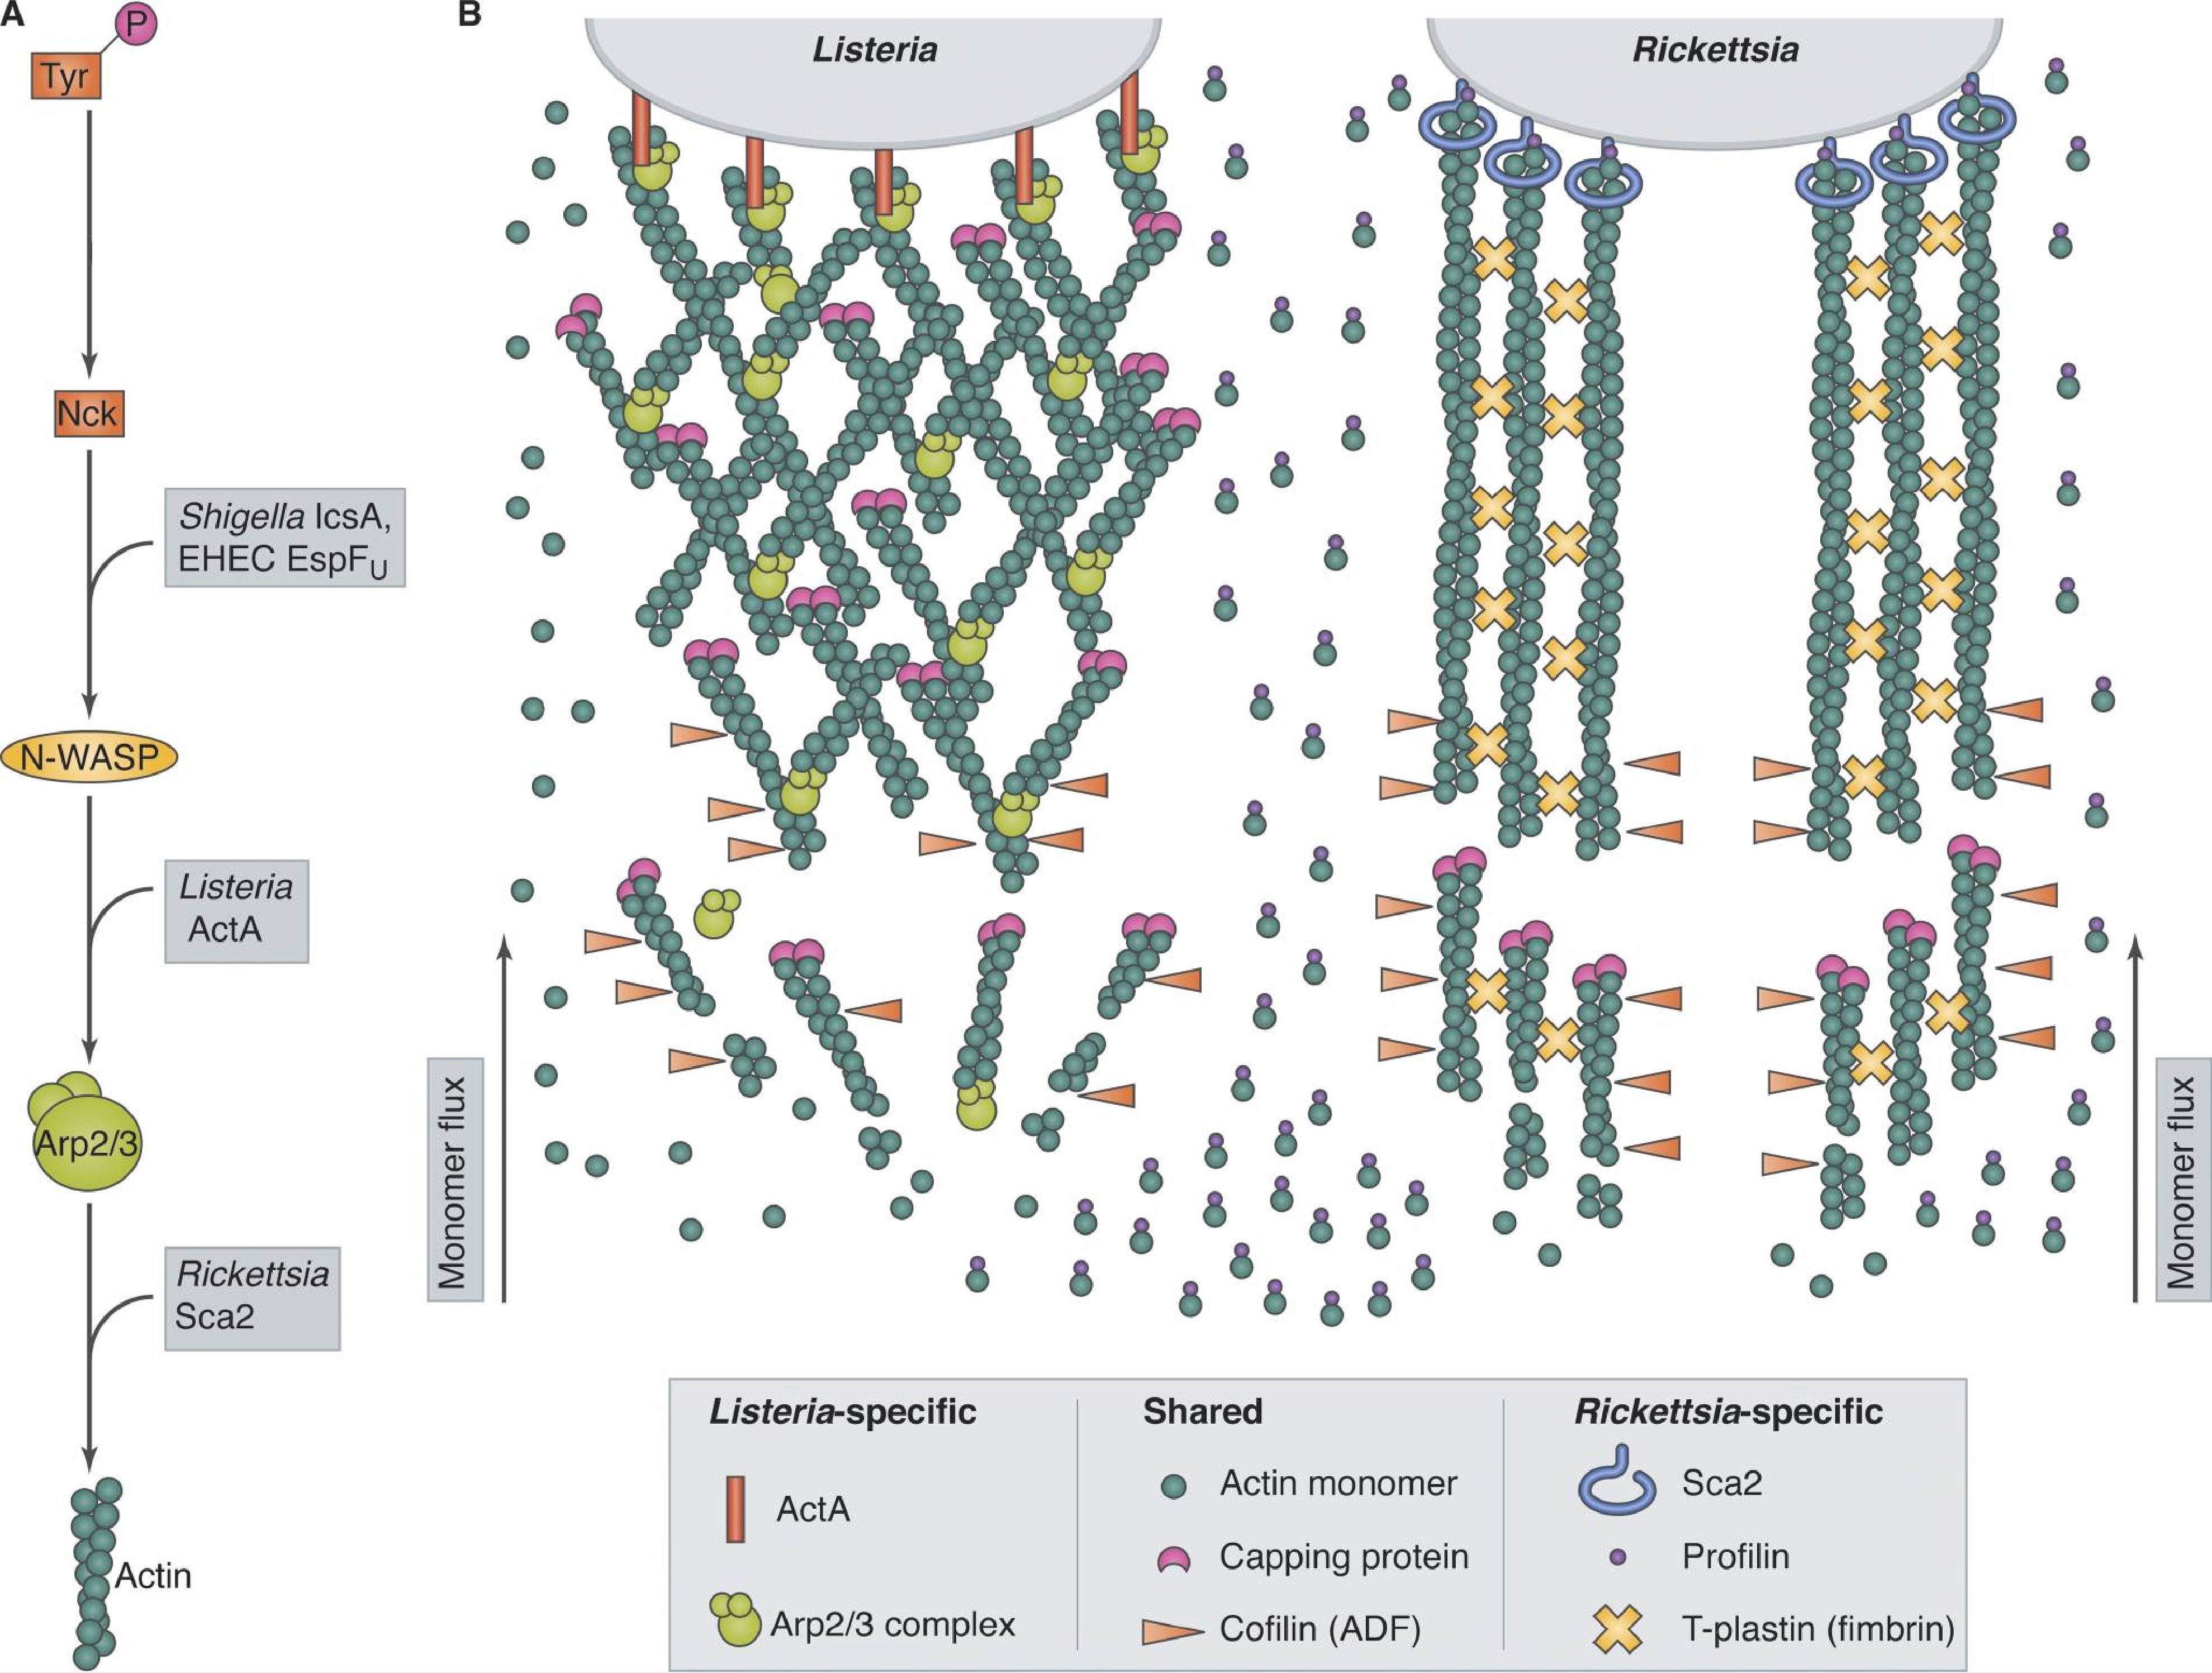
\includegraphics[width=0.95\textwidth]{actin-motility}
  \caption[Mechanisms of \acrlong{abm} in several intracellular bacterial pathogens.]{The capability for \acrfull{abm} evolved independently in several intracellular bacterial pathogens. (A) The entry points into the cellular actin assembly pathway vary, with some organisms providing their own \acrfull{npf} (\textit{Listeria} and \textit{Rickettsia}), while others rely on cellular \acrshort{npf} (\textit{Shigella} and \acrlong{ehec}). The branching pattern of actin tails differs between organisms relying on cellular \acrshort{arp23} (\acrlong{arp23}) from those capable of \acrshort{arp23} independent \acrshort{abm} (B). Cofilin is responsible for actin depolymerization, profilin is a regulatory protein catalyzing the exchange of \acrshort{adp} to \acrshort{atp} and fimbrin crosslinks actin strands into bundles. Adapted from \citet{Haglund2011}.}
  \label{fig:actin-motility}
\end{figure}

\phantomsection
\label{actin-motility}
\paragraph{\Acrfull{abm}.}
As for large viruses, free diffusion within the cytoplasm is not readily possible for bacteria and a feature common to most cytosolic bacterial is 
\cgls{abm}. Actin monomers exist in two forms, G-actin (globular) and F-actin (filamentous). \cGls{atp} binds G-actin, and upon formation of a trimeric nucleus the nascent chain grows in both directions while \cgls{atp} is hydrolyzed. When the chain reaches a certain length, growth becomes directional and association of monomers at the plus end compensates for dissociation of monomers at the minus end. This leads to a self-sustaining scheme described as treadmilling. Limiting to actin polymerization is the kinetically unfavorable nucleation step and in vivo, this is stimulated by cellular factors such as \cgls{arp23} which require activation by \cglspl{npf}, including members of the \cgls{wasp} family \citep{Stevens2006,Haglund2011}.

\cGls{abm} exhibiting pathogens can be divided into two groups depending on whether they provide \cglspl{npf} of their own or recruit host cell \cglspl{npf}. Expression of \acrrev{acta} by \textit{L. monocytogenes} is both necessary and sufficient for \cgls{abm} as shown in a cell free system using \cgls{acta} coated beads, actin, \cgls{arp23}, CapZ, cofilin and \cgls{atp}. No cellular \cgls{npf} is required as \cgls{acta} mimics \cgls{wasp} and directly activates \cgls{arp23}. \textit{Rickettsia} are among the few pathogens capable of \cgls{abm} without relying on \cgls{arp23}, leading to formation of actin tails with a distinct morphology. The formin-like protein Sca2 directly interacts with actin and RickA, exhibiting some homology to \cgls{wasp} can act as \cgls{npf}. A further organism that mimics cellular \cgls{npf} is \textit{B. pseudomallei}, which is capable of BimA-mediated, \cgls{arp23} independent actin polymerization.

Bacterial pathogens that rely on cellular \cgls{npf} instead of supplying their own include \textit{S. flexneri}, \textit{Mycobacterium marinum}  and \cgls{ehec}. In \textit{S. flexneri} infection, bacterial \acrdbl{ics}[A], capable of recruiting \cgls{n-wasp}, is the only required bacterial factor for triggering \cgls{abm}. By inducing conformational changes in \cgls{n-wasp}, \acrdbl{ics}[A] is thought to mimic activation by \cgls{cdc-42}, allowing for association of \cgls{n-wasp} with \cgls{arp23}. Details of \cgls{abm} in \textit{M. marinum} are less well known but as it is both \cgls{wasp} and \cgls{arp23} dependent, it is assumed that the employed mechanism is similar to that of \textit{S. flexneri}.

Both \cgls{ehec} and \cgls{epec}, while not intracellular pathogens, are able to induce cytosolic actin polymerization. By inserting the transmembrane protein \cgls{tir} into the plasma membrane they are able to initiate actin polymerization via the same pathway as \cgls{abm}, leading to the formation of pedestals protruding outwards. This is thought to provide means of extracellular motility. Intercellular motility by \cgls{abm} capable bacteria is achieved by pushing against the host cell membrane into the neighboring cell body until being engulfed in a double membrane vacuole that is subsequently lysed.

\phantomsection
\label{autophagy}
\paragraph{Autophagy.}
The basic catabolic cellular mechanism of autophagy is initiated as response to stress signals such as nutrient starvation, damaged cellular compartments and foreign particles. Cytoplasmic components marked for degradation are captured by the double-membrane autophagosome, intended for fusion with lysosomes. As cellular defense mechanism, cytosolic pathogens are targeted by selective autophagy in a process also related to as xenophagy. Bacterial response can be categorized as interference with the autophagy pathway, evasion of autophagy recognition or escape from the autophagosome \citep{Ham2011,Huang2014}.

\textit{S.} typhimurium, while not usually considered a cytosolic pathogen, has been shown to occasionally escape the phagocytic vacuole and replicate in the cytosol. Membrane damage triggers an amino acid starvation response that activates autophagy signaling by relocating \cgls{mtor} from the late endosome to the cytosol. The bacteria respond via unknown action probably involving \acrshort{spi}[-2] \cgls{t3ss} secretions that are able to restore both the cytosolic amino acid pool and \cgls{mtor} localization, successfully inhibiting autophagy. Further examples of autophagy-initiation signaling inhibition are provided by \textit{M. tuberculosis} which is able to produce \cgls{eis}, an inhibitor to production of \cgls{ros} needed as an autophagy signal. Furthermore, bacterial toxins apt to interfere with \cgls{camp} regulation can block autophagy in mammalian cells.

After autophagy has been initiated, the procedure can still be modified as shown by \textit{L. pneumophila} and \textit{S. flexneri}. The former organism secretes RavZ via \cgls{t4ss} which decouples the autophagy marker LC3 from the phagosomal membrane while the latter expresses \acrdbl{vir}[A] via \cgls{t3ss}, a \cgls{gap}capable of inactivating the autophagy regulator \ACRshort{rab}[1]. Another group of bacteria prevent or delay lysosome fusion and accumulate in non-degradative vacuoles at neutral pH. Examples include \textit{M. marinum}, \textit{Chlamydia trachomatis}, \textit{Yersinia pestis} and \textit{Helicobacter pylori}.

Evasive measures have been suggested to be employed for \textit{S. flexneri} and \textit{L. monocytogenes}. \Acrdbl{ics}[B] of \textit{S. flexneri} and \cgls{acta} of \textit{L. monocytogenes} have been implicated of masking the bacteria from autophagy targeting mechanisms and it has been suggested that \cgls{abm} might somehow facilitate hiding from host cell detection. By also currently unknown means, \textit{B. pseudomallei} can escape the phagosome of an autophagy-related process, possibly involving BopA secretion via \cgls{t3ss}.

\section{Select Bacterial Pathogens}

A total of 5 bacterial pathogens were selected for study within the InfectX \cgls{rtd} project by SystemsX. This section shortly describes each organism in terms of microbiological features, pathogenesis, epidemiology and diseases caused in humans. For each organism, a chapter of \citet{Gillespie2006} serves as basis and is supplemented by one or two review articles referenced in the first paragraph of each section.

\subsection{\textit{Bartonella henselae}}

\textit{Bartonella henselae} is a short, rod shaped, unflagellated proteobacterium, phylogenetically closely related to the genus \textit{Brucella}, presenting 94.4\% 16S \cgls{rrna} gene sequence homology, compared with \textit{Brucella abortus}. The Gram-negative bacillus is a facultative anaerobic, intracellular parasite and was first described in 1992. Relatively harmless for healthy humans, infections can become life threatening in immunocompromised patients, making the species an important opportunistic pathogen \citep{Anderson1997,Harms2012}.

\paragraph{Diseases.}
In immunocompetent humans, infection with \textit{B. henselae} can lead to a condition known as \cgls{csd}. As the name suggests, most patients report being in contact with a cat and transmission often occurs through scratches and bites. Affecting primarily children and young adults (80\% are 21 or younger), the self limiting infection typically presents itself with lymphadenopathy. Most patients remain afebrile and do not report feeling ill, with low-grade fever and malaise shown in roughly 30\% of the cases. Recovery from uncomplicated \cgls{csd} usually takes 2 to 6 months and requires no specific treatment.

Possible complications include Parinaud's oculoglandular syndrome (granulomatous conjunctivitis in one eye and parotid lymphadenitis on the same side), splenomegaly and hepatic or splenic abscesses, accompanied by fever, weight loss, fatigue and malaise. In 1 to 7\% of the cases, the disease spreads to the central nervous system, leading to encephalopathy, but recovery is usually rapid (within several weeks).

Infections with \textit{B. henselae} tend to have more severe consequences for immunocompromised patients, such as bacillary angiomatosis, bacteremia and endocarditis. \cGls{aids} patients suffering from \cgls{csd} usually experience severe, progressive disease with infection spreading systematically and without appropriate treatement, fatal outcome. \textit{Bartonella} \acrshort{spp} are the only prokaryotes known to be able to induce angiogenic tumors such as bacillary angiomas, which may involve skin, respiratory or gastrointestinal epithelia, hart, liver, spleen, bone marrow, muscles, or lymph nodes. Bacteremia may lead to inflamed heart valves, usually requiring endocarditic patients to have heart valve replacement surgery.

\begin{figure}
  \centering
  \includegraphics[width=0.75\textwidth]{bartonella}
  \caption[Bacterial effectors of \textit{B. henselae}, secreted by a \cgls{t4ss} into the host cytosol.]{Several effectors secreted by a \acrshort{t4ss} apparatus in \textit{B. henselae} infection serve as virulence factors for colonization of the intracellular replicatory niche. The ones best characterized alongside their phenotype are schematically summarized. Adapted from \citet{Harms2012}.}
  \label{fig:bartonella}
\end{figure}

\paragraph{Pathogenesis.}
\textit{B. henselae} are capable of intracellular growth in both epithelial cells and erythrocytes but the focus of this section lies on infection of the former cell type. Initial attachment is mediated by the \cgls{taa} BadA which is capable of both interacting with the \cgls{ecm} and \textbeta$_1$-integrin, followed by effector secretion via the bacterial \cgls{t4ss} \acrshort{vir}[B\slash D4]. For host cell entry, two mutually exclusive mechanisms have been described. Either single bacteria or small groups are phagocytosed via a zipper-like mechanism or large clusters are internalized in a unique cellular structure termed an invasome. While invasome formation is a slow process, taking 16 to 24 hours, \cglspl{bacv} resulting from endocytosis are visible within minutes. It has been suggested that inhibition of endocytosis by either a combination of effector proteins \acrshort{bep}[C] and \acrshort{bep}[F] or the exclusive action of \acrshort{bep}[G] is crucial to invasome formation as it allows for aggregation of bacteria on the cell surface. Not the activity of effector proteins but the clustering of cellular receptors may trigger large-scale internalization (see figure \ref{fig:bartonella}).

Pathological angiogenesis can be induced by a set of agonistic and antagonistic effectors. While \acrshort{bep}[G] is a strong inhibitor to angiogenesis, both \acrshort{bep}[D] (weakly) and \acrshort{bep}[A] (strongly) promote sprouting of blood vessels. Although the exact mechanism of induction and regulation remains to be uncovered, the secretion of \cgls{vegf} has been demonstrated in vasoproliferative tumors caused by \textit{B. henselae}. Furthermore, transcriptional promotion of various factors supporting angiogenesis, including \cgls{icam-1}, \cgls{il-8} and angiopoietin-2 by bacterial effectors are unanimously agreed upon. Curiously, secretion of \cgls{vegf} by infected endothelial cells has so far not been possible to show.

Inhibition of apoptosis is decisive to intracellular survival and it is assumed that \acrshort{bep}[A] is capable of \cgls{camp} mediated antiapoptotic action. The role of two further effectors that have been identified as part of the \cgls{t4ss} in \textit{B. henselae}, \acrshort{bep}[B] and \acrshort{bep}[E], are unknown, as are the mechanisms leading to activation of proinflammatory signaling via \acrrev{nf-kb}.

\paragraph{Epidemiology.}
The role of cats and in particular kittens, as reservoirs to \textit{B. henselae} has been firmly estabished. Infected felines are asymptomatic and show no signs of illness. Cat fleas (\textit{Ctenocephalides felis}) serve as vectors to spread the bacteria among cats and have also been suspected of infecting humans. The main path of transmission to humans however, is through scratches and bites by infected cats. \textit{B. henselae} has also been found in ticks and tick bites prior to contraction of \cgls{csd} have been reported.

In the United States, 24000 cases of \cgls{csd} are reported yearly, yielding 2000 hospital admissions with an estimated health care cost of \$12 million. Children are more likely to be affected (80\%) and incidence is higher in males (60\%). The seasonal pattern (occurrences higher in fall\slash winter) is attributed to cat mating patterns, as well as pet acquisition fluctuations.

\subsection{\textit{Brucella abortus}}

The Danish physician David Bang first isolated \textit{Brucella abortus} in 1895 from cyetic cattle tissue, investigating a contagious disease causing abortions in cows. \textit{B. abortus} are small, unflagellated proteobacteria with a cell wall consisting of an outer layer (\SI{9}{\nano\meter}) of \cgls{lps} and an inner layer (3--\SI{5}{\nano\meter}) of muramyl mucopeptide complexes. The Gram-negative cocobacilli appear to have evolved from free-living, soil-dwelling species and are closely related to other human pathogens such as \textit{Bartonella} \acrshort{spp}, based on 16S \cgls{rrna} sequences. Brucella species were investigated for possible use as warfare agents in the mid 20th century by several armed forces. \citep{Atluri2011,VonBargen2012}

\paragraph{Diseases.}
Brucellosis is a human disease caused by several pathogenic \textit{Brucella} species, most importantly \textit{B. abortus}, \textit{B. melitensis}, \textit{B. canis} and \textit{B. suis}. Onset may be acute or insidious and due to protean symptoms, diagnosis based on clinical presentation alone is difficult. The febrile disease is generalized and may involve many parts of the body, including nervous, skeletal, gastrointestinal, cardiovascular, respiratory and genitourinary systems. Furthermore, as the bacteria spread to other reservoir hosts via their reproductive systems, persistence of infection is crucial to the pathogen and it comes as no surprise that brucellosis can manifest as a chronic disease in humans too.

\hyphenation{as-the-ni-a an-o-rex-ia nau-sea ma-laise ar-thri-tis he-p-ato-mega-ly splen-o-meg-aly epi-di-dymo-orch-it-is pul-mon-ary bron-chit-is pneu-mo-nia en-do-cardit-is men-ingit-is men-in-go-en-ceph-al-it-is}

Fever is the most consistent sign of \textit{Brucella} infection and depending on what specific organs are affected, further symptoms include asthenia, anorexia, nausea, malaise, arthritis, epididymo-orchitis in males, hepatomegaly, splenomegaly and pulmonary manifestations such as bronchitis or pneumonia. A rare complication (less than 2\%), albeit the most lethal, is infective endocarditis. Invasion of the nervous system develops in less than 5\% of cases and often results in meningitis or meningoencephalitis with good prognosis under antimicrobial treatment.

\paragraph{Pathogenesis.}
Host entry occurs primarily via the digestive system but is also possible through the respiratory tract or skin lesions. Via the gastrointestinal route, \textit{Brucella} \acrshort{spp} target Peyer's patches (lymphoid nodules localized towards the end of the small intestine) and must therefore pass through acidic conditions in the stomach. This is facilitated by expression of two ureases capable of hydrolyzing urea and producing a protective bicarbonate buffering system. When entering through the respiratory system, \textit{B. abortus} target alveolar macrophages which serve as access point to the lymphatic system therefore facilitating systematic spread.

In order to persist at systemic sites, both active and passive mechanisms for evading the immune system are in place. \cGls{lps} of the outer cell wall disguises the bacteria from \cglspl{tlr} and expression of two proteins containing \cgls{tir-1} domains actively interferes with \cgls{tlr} signaling.

Uptake by macrophages happens via phagocytosis, which is either triggered by nonopsonized bacteria through a lipid raft mediated mechanism or by opsonization. Although opsonin marked bacteria are 10-fold more likely to be ingested, the number of pathogens reaching their destination within the host cell is higher for nonopsonized bacteria. Still, most bacteria (up to 90\%) are unsuccessful in evading their digestion and only very few are able to establish a replicative niche. Apart from professional phagocytes, epithelial cells may also be infected and the following paragraphs focus on this particular cell type.

\begin{figure}
  \centering
  \includegraphics[width=0.75\textwidth]{brucella}
  \caption[Schematic representation of the \textit{B. abortus} intracellular life cycle.]{Schematic representation of the \textit{B. abortus} intracellular life cycle, from cell entry via maturation of the \acrlong{brcv} to establishing an intracellular replicatory niche. Interaction with many different cellular compartments of the endocytic pathway and the \textit{cis} Golgi network are required for successful infection. Adapted from \citet{VonBargen2012}.}
  \label{fig:brucella}
\end{figure}

Initial attachment is mediated by unknown eukaryotic receptors containing sialic acid residues that interact with \cgls{sp41}. While involvement of bacterial \acrshort{hsp}60 and and \cgls{prpc} has been proposed, this remains controversial. Maturation of early \cglspl{brcv} is important for successful infection as preventing acidification (through addition of bafilomycin A) or fusion with lysosomes (through suppression of the late-endosomal \acrshort{gtp}[ase] Rab7) interferes with bacterial replication. This observation can be explained with acid serving as a trigger for expression of the \cgls{t4ss} \acrdbl{vir}[B]. However fusion events with late endosomes and lysosomes are only limited and under bacterial control.

Upon acquisition of late endosomal markers and acid initiated expression of \cgls{t4ss}, fusion with autophagic vacuoles occurs, leading to formation of an autophagosome-like compartment. Subsequent interactions with \cgls{er} exit sites, mediated by secreted effectors, further modify the \cgls{brcv} into an \cgls{er}-derived vacuole, coated with ribosomal particles. At this stage, located within the \cgls{ergic}, the replicatory niche is reached. Blocking the small \acrshort{gtp}[ase] Sar1 inhibits intracellular replication by preventing acquisition of \cgls{cop-2}, participating in anterograde \cgls{er}--Golgi transport, by ER-exit vesicles. Furthermore, the small \acrshort{gtp}[ase] Rab2, involved in ER--cis-Golgi traffic, is required for maximal proliferation, illustrating the dependence of \textit{Brucella} on intercepting vesicular traffic.

Despite multiplying intra-cellularly in high numbers, host cells are kept alive and are even able to replicate despite infection. \textit{Brucella} species are able to interfere with apoptosis, maintaining their replicatory niche, protected from immune response. It remains unknown what happens when the hosts capacity for freeloaders is reached, as well as how bacteria exit the host cell and spread.

\paragraph{Epidemiology.}
Preferred natural reservoir species for \textit{B. abortus} are cattle (\textit{Bos taurus} and \textit{Bos indicus}) and almost all parts of the world are affected. The disease exists in both domestic and wild animals and is most prevalent in Mediterranean countries, North Africa, throughout the Middle East, India, Central Asia, as well as South and Central America. Zoonosis most often occurs through ingestion if unpasteurized milk products but airborne transmission is also possible, putting professionals involved in animal husbandry at risk. Vertical transmission among reservoir hosts can occur through lactation and horizontal transmission is facilitated by mating and placental discharge associated with aborted gestation. Human-to-human transmission is rare (but has been suspected to be possible via sexual intercourse), making humans dead-end hosts. As opposed to \textit{Bartonella}, immunodeficient patients do not seem to be especially susceptible towards \textit{Brucella} infections.

Worldwide, an estimated 500000 new cases of brucellosis occur annually, making it one of the most prevalent zoonoses. Although usually susceptible to combined antibiotic therapies of at least two agents (usually a tetracycline antibiotic combined with an aminoglycoside or rifampin), untreated brucellosis leads to a high degree of morbidity, leading to being classified a neglected zoonosis by the \cgls{who}.

\subsection{\textit{Listeria monocytogenes}}

The short, Gram-positive bacilli are non-sporeforming facultative anaerobes, capable of growing in a wide temperature range (0--\SI{50}{\celsius}) and in many different environments. Flagellation is temperature dependent with flagellin being expressed and assembled into peritrichous flagella around 20--\SI{25}{\celsius} but not at \SI{37}{\celsius}. First described in 1924 by Murray after isolation from lymph glands of diseased laboratory animals, the pathogen was found to also infect humans four years later. For much of the time since, listeriosis was considered a rare zoonotic disease and did not receive much attention. It was not until the 1980s, when several food-borne listeria outbreaks caused a shift in interest towards the pathogen, which has since become a well studied facultatively intracellular parasite \citep{Farber1991,Cossart2014}.

\paragraph{Diseases.}
Maternal and neonatal listeriosis accounts for almost half of all infections. Listeriosis in pregnancy typically manifests in bacteraemia and presents as a self-limiting febrile disease with flu-like symptoms. Many cases, however are asymptomatic and the first sign of infection is abortion or neonatal listeriosis. Maternal infection does not necessarily carry over to the fetus, especially if proper chemotherapy is administered. Perinatal incidences are divided into early and late onset (\textgreater 5 days after parturition), with former cases typically resulting in septicemia and latter cases in meningitis. While in early onset cases the predominant route of transmission is transplacental, the situation is less clear in late onset cases. Both the maternal genital tract during child birth and environmental sources have been implicated. Despite antibiotic treatment, overall mortality rates of 30--40\% are typical and prognosis for early onset disease is worse, as it is often associated with preterm birth and advanced stage of infection. 

Among adults, most cases of listeriosis occur in T-cell deficient individuals. \cgls{hiv} infection, for example, increases incidence 150--300 fold compared to general population control groups. Predisposing conditions include lymphoreticular neoplasms, deliberate immunosuppression (e.g. antirejection treatment after organ transplants), alcoholism and diabetes mellitus. Despite increased susceptibility caused by immunodeficiency, roughly 30\% of all infections affect immunocompetent individuals. In healthy adults, consumption of food contaminated with \textit{L. Monocytogenes} can either lead to self-limiting febrile gastroenteritis with short incubation time (\textless \SI{24}{\hour}) or invasive listeriosis with much longer incubation periods (3--4 weeks). The systemic form of infection often manifests as bacteraemia or as a neurological infection, but can also involve endocarditis and spread to other parts of the body. Central nervous system involvement occurs in as much as 75\% of cases and either presents as meningitis or encephalitis. Mortality rates of 35--45\% have been reported for listeriosis in adults.

\begin{figure}
  \centering
  \includegraphics[width=0.95\textwidth]{listeria}
  \caption[A selection of features relevant for infection of epithelial cells by \textit{Listeria}.]{\textit{Listeria} enter host epithelial cells via a zipper-type entry mechanism mediated by the bacterial internalins \acrshort{inl}[A] and \acrshort{inl}[B]. In order to reach the cytosolic replicatory niche, lytic \cgls{llo} is secreted and \cgls{abm} provides means of locomotion. Evading host detection and maintaining a permissive environment is controlled by several bacterial effector molecules including \acrshort{inl}[C], \acrshort{inl}[K] and LntA. Adapted from \citep{Cossart2014}.}
  \label{fig:listeria}
\end{figure}

\paragraph{Pathogenesis.}
The predominant entry path for \textit{L. Monocytogenes} into the human body is via the gastrointestinal tract, where Peyer's patches are targeted. The bacteria can induce cellular uptake, by non-phagocytic host cells via expression of cell-surface associated interanlins through a zipper-type entry program (see section \ref{zipper-mechanism}). The cellular receptor for bacterial internalin \acrshort{inl}[A] is E-cadherin and internalin \acrshort{inl}[B] interacts with the receptor tyrosine kinase c-Met. Upon internalization, the phagosomal membrane is lysed, mediated by secretion of listerial haemolysin \cgls{llo} in a cholesterol dependent mechanism whereby \cgls{llo} monomers associate, oligomerize and form \SI{35}{\nano\meter} pores. \cgls{llo} is acid activated with an optimum around pH 5.5, which is reached in late endosomes. Moreover, \cgls{llo} is required for autophagy modulation (see section \ref{autophagy}) and has been implicated in regulating inflammatory response.

Growth and replication occur in the cytoplasm and \cgls{acta} mediated \cgls{abm} (see section \ref{actin-motility}) provides means of intracellular and intercellular movement. Adjacent cells can be entered by pushing against the plasma membrane and forming a pseudopod-like structure which in turn is taken up the neighbor. The resulting double-membrane vacuole is escaped by cytolysis, again dependent on \cgls{llo}.

Several mechanisms for persistence within the replicatory niche have recently been uncovered. Down-regulation of the host pro-inflammatory response is dependent on secretion of \acrshort{inl}[C], a virulence factor of the internalin family which prevents phosphorylation of \cgls{nf-kb} and thus prevents nuclear translocation. Both \acrshort{inl}[K] and \cgls{acta} are associated with \cgls{abm} and are simultaneously involved in autophagy evasion. Finally, mechanisms for several epigenetic host modifications have been demonstrated. Both \cgls{llo} action and Met-binding during invasion, trigger histone modifications and upon entry, the virulence factor LntA localizes to the nucleus where it interacts with the newly characterized chromatin component BAHD1. While illustrating that \textit{L. monocytogenes} is capable of reprogramming host gene expression, the exact implications of this capability have yet to be elucidated.

In an extracellular setting, haemolysins serve to rupture erythrocytes in order to generate free iron, a limiting growth factor. Furthermore the nonspecific immune system has to be evaded and haemolysins have also been shown to be cytotoxic towards leukocytes. Additionally, expression of bacterial superoxide dismutase mitigates the effect of free superoxide radicals which play an important role in killing phagocytized bacteria.

\paragraph{Epidemiology.}
Incidence of listeriosis has initially been increasing since its recognition as food-borne disease but effects of awareness and diagnostic methods are unclear. While typically long incubation periods do pose difficulties for clinical diagnosis, the number of susceptible individuals is on the rise and certain aspects modern processing and handling of foods may be beneficial for growth of \textit{L. Monocytogenes}. Disease rates of 2--15 cases per million population per year have been reported and listeriosis is among the leading case of lethal food-borne pathogen infections. Most recent data, however suggests, that incidence is decreasing again.

Due to its non-fastidious lifestyle, \textit{L. Monocytogenes} has been isolated from a wire array of ecological niches, including soil, sewage and water (both fresh water bodies and estuaries). High persistence (up to 4 years) in soil samples is problematic when contaminated manure is used as fertilizer and biofilm formation poses challenges for eradication from food processing plants. Additionally, the ability to grow in refrigerated foods and resistance towards heat treatment such as pasteurization warrant alertness and special preventive care. Many different foods have been implicated in listeriosis outbreaks, including vegetables (potatoes, radishes and celery), seafood (shrimp, crabmeat and smoked fish), diary products (soft cheese, pasteurized and unpasteurized milk) and meats (poultry, various types of sausages and pâté).

Despite high prevalence in food (studies have found 20--80\% of meat product samples and 1--10\% of diary product samples contaminated with \textit{L. Monocytogenes}), comparatively few successful infections occur. The bacteria are ingested frequently in small doses and stool sample examinations suggest that 10-70\% of investigated populations could be intestinal carriers. While the minimum infectious dose has not been settled definitively, approximations range from $10^6$ to $10^9$ bacteria.

\subsection{\textit{Salmonella} Typhimurium}
\textit{Salmonella} are non-sporulating, Gram-negative bacilli, belonging to the family Enterobacteriaceae. The motile bacteria are able to produce peritrichous flagella and diameters span 0.7 to \SI{1.5}{\micro\meter} while typical lengths range from 2 to \SI{5}{\micro\meter}. They are closely related to the genus \textit{Escherichia}, showing only 15\% chromosomal sequence disparity. Currently, two distinct species, \textit{S. bongori} and \textit{S. enterica}, within the genus \textit{Salmonella} are recognized, both of which are pathogenic towards a wide array of hosts. \textit{S. enterica} is further divided into 6 subspecies, the most relevant of which for human and domestic animal hosts being \textit{enterica}. A large number of serovars (more than 2500) for \textit{S. enterica} \acrshort{subsp} \textit{enterica} have been characterized and due to an originally mistaken classification as separate species, some serovars are designated with shortened names. \textit{S.} Typhimurium, therefore is shorthand for \textit{S. enterica} \acrshort{subsp} \textit{enterica}, serovar Typhimurium and to emphasize that Typhimurium is not a species description it is not italicized.

The first description of the genus \textit{Salmonella} dates back to an investigation into swine fever led by Salmon and Smith in 1885. The newly isolated bacterium was wrongly proposed as the etiological agent, as the disease later tuned out to be caused by a virus \citep{Fabrega2013,Haraga2008}.

\paragraph{Diseases.}
Two distinct disease patterns are associated with \textit{Salmonella} \acrshort{spp} infections, typhoid fever and salmonellosis. While the former is exclusively caused by the serovars Typhi and Paratyphi, the latter is associated with several serovars, the most frequent being Enteritidis and Typhimurium, accounting for 65\% and 12\% of cases worldwide. The current and following sections will not discuss typhoid fever.

Salmonellosis is a diarrheal disease with a short incubation period of 6--24 h, followed by nausea, vomiting, loose or liquid bowel movements, abdominal cramps and fever. Clinical features are similar to those of dysentry and other gastroenteric disease and can include bloody and mucosal stool. In most cases, the infection is self-limiting and symptoms fade away within 4 to 7 days. The most common complication is bacteraemia, which presents in 5\% of cases and is more likely to develop in children, especially if malnourished, and immunocompromised individuals. Further manifestations of invasive infections include meningitis, osteomyelitis, cholangitis, pneumonia and endocarditis. While mortality in immonocompetent hosts in developed countries is as low as 0.1\%, it can increase to 77\% for \cgls{hiv} positive patients in undeveloped countries.

\begin{figure}[t]
  \centering
  \includegraphics[width=0.7\textwidth]{salmonella}
  \caption[Overview of mechanisms for infection of epithelial cells by \textit{Salmonella} and for establishing an intracellular replicatory niche.]{Two separate \cgls{t3ss} are encoded in the \textit{Salmonella} genome which serve as central virulence factors at different stages of infection. \cGls{t3ss} of \acrshort{spi}[-1] secretes effectors required for triggering internalization (A), while \cgls{t3ss} of \acrshort{spi}[-2] is critical for maturation of the phagosome into a replication permissive \cgls{scv}. Figures adapted from \citet{Haraga2008}.}
  \label{fig:salmonella}
\end{figure}

\paragraph{Pathogenesis.}
In order to reach the small intestine, ingested \textit{S.} Typhimurium first have to defy the hostile environment of the stomach. A set of proteins, summarized as \cgls{atr} helps mediate the acidic conditions and improves survival rates. The remaining bacteria subsequently end up in the small bowel and target epithelial cells, with preference towards \cgls{m-cells}. Flagellar motility enables penetration of intestinal mucus secretions and improves the chance of reaching the intestinal walls where adhesion can be established. Fimbriae are important attachment factors, capable of interaction with host-cell laminin and fibronectin and provide an initial platform for pathogen induced phagocytosis via trigger mechanism (see section \ref{trigger-mechanism}). 

\textit{S.} Typhimurium utilize two separate \cgls{t3ss} systems for host-cell colonization, the first of which (\acrshort{t3ss} of \acrshort{spi}[-1]) mediates invasion. In addition to strengthening initial interactions attaching the pathogen to its target, the needle like structure serves as delivery mechanisms, capable of injecting effector proteins, including \acrdbl{sop}[E], \acrdbl{sop}[E2], \acrdbl{sop}[B] and \acrdbl{sip}[A]. \Acrdbl{sop}[E] serves as \cgls{gef} and activates Rho \acrshort{gtp}[ases] \cgls{rac-1} and \cgls{cdc-42} via \acrshort{gdp}\slash \acrshort{gtp} exchange, which in turn initiate cytoskeletal rearrangements. \Acrdbl{sop}[E2] is a further \cgls{gef}, highly homologous to \acrdbl{sop}[E] and it is assumed to provide some level of redundancy for \acrdbl{sop}[E] as shown by \textit{Salmonella} strains missing the \acrdbl{sop}[E] gene. \Acrdbl{sop}[B] is a phosphatase, capable of hydrolyzing various substrates, including \cgls{i13456p5}, which has been linked to intestinal fluid secretion causing diarrhea and \cgls{pi45p2}, involved with membrane rigidity. 

The actin binding proteins \acrdbl{sip}[A] and \acrdbl{sip}[C] stimulates actin polymerization and promotes membrane ruffling, yielding a macropinocytic pocket. \cGlspl{mapk} initiate pro-inflammatory response via \cgls{nf-kb} signaling, leading to the expression of \cgls{il-8}. Furthermore, damage the tight junctions make the epithelial barrier permissive to bi-directional leakage. After internalization, actin structure is restored and \cgls{mapk} signaling down regulated by \acrrev{sptp}, \acrshort{ssp}[H1] (\acrlong{ssp} H1) and \acrrev{avra}.

Upon engulfment, maturation of the phagosome and fusion with lysosomes have to be prevented. Unlike other pathogens that escape the digestive mechanisms of phagocytic vesicles by moving to the cytosol, \textit{Salmonella} replicate inside phagosome-derived \cglspl{scv}. In this setting, the second translocation complex (\cgls{t3ss} of \acrshort{spi}[-2]) is activated, and used to secrete effectors, including \acrdbl{ssa}[B] and \acrdbl{sif}[A], capable of interacting with vesicular trafficking mechanisms and guiding the \cgls{scv} away from its original degradation pathway. Furthermore \cgls{t3ss}-2 translocated effectors such as \acrshort{ssp}[H2], \acrdbl{spv}[B] and \acrdbl{sse}[L] induce actin polymerization events, which relocate the \cgls{scv} toward a perinuclear position. A last step in creating the intracellular niche needed for replication, is formation of \GLSpl{sif}, extending outwards from the \cgls{scv}. \cGls{t3ss}-2 secretes effectors such as \acrdbl{sif}[A], PipB2, \acrdbl{sse}[F] and \acrdbl{sse}[G], which mediate the microtubule dependent processes by bundling and accumulating filaments and regulating microtubule motor function.

\paragraph{Epidemiology.}
The global disease burden caused by nontyphoidal salmonellosis is estimated at 90 million cases per year and 150000 deaths. Incidence rates are highest in East and Southeast Asia (up to 4000 cases per 100000 population per year) and both developed and undeveloped countries are affected (incidence rates in Africa are estimated at 320 while estimates for Europe are around 690 cases per 100000 population per year). An estimated 80.3 million or 86\% of reported cases are food borne \citep{Majowicz2010}.

In order to control \textit{Salmonella} outbreaks, preventive measures in food production and processing is of major importance. This starts with disease containment in domestic animals, such as vaccination of chickens, enforcing  hygiene standards in manufacturing and distribution facilities and ends with proper preparation, exploiting heat sensitivity of the organisms. As the main route of transmission is fecal--oral, good sanitary infrastructure, treatment of sewage and water processing are crucial prerequisites in combating outbreaks of salmonellosis.
% minimum infectious dose + biofilm formation leading to asymptomatic presistence

\subsection{\textit{Shigella flexneri}}
Shigellae are small, non-sporeforming, Gram-negative bacilli and belong to the family \textit{Enterobacteriaceae}, along with \textit{Escherichia}, \textit{Salmonella} and \textit{Yersinia}. While flagellar genes are present and their expression is observed under certain conditions, the bacteria are usually described as non-motile and unflagellated. The facultative intracellular parasite shows strong specificity towards human hosts where it typically infects the lower gastrointestinal tract.

\textit{Shigella dysenteriae} was identified as the etiological agent of dysentery by Shiga in 1897 during an epidemic in Japan with 91000 reported cases and a \textgreater 20\% mortality rate. \textit{S. Flexneri} was first described by Flexner in 1900, while investigating diseases endemic to the Philippines. Recent genetic studies suggest, that \textit{Shigella} \acrshort{spp} belong to the species \textit{Escherichia coli}, rather than forming a distinct genus, as only marginal sequence divergence (1.5\%) between \textit{E. coli} and \textit{S. Flexneri} was found \citep{Schroeder2008,Croxen2010}.

\paragraph{Diseases.}
Bacillary dysentery is an acute infection of the intestine. Mild cases of the disease are self-limiting and afebrile with diarrhea and possibly vomiting as the only symptoms. In as little as 24 hours after onset, bowel movements usually begin to normalize and the condition is resolved within a few days. More severe cases are accompanied by strong abdominal cramps, fever and watery diarrhea containing blood and mucus, indicative of injury to the intestinal epithelium. While still usually self limiting in healthy individuals, recovery takes 10--14 days and relapses are possible. In immunocompromised patients, young children, especially if malnourished, and elderly individuals, life threatening complications including bacteraemia, renal failure, intestinal perforation and toxic megacolon are more frequent. Involvement of the central nervous system and respiratory tract is rare.

Administration of antibiotics is not recommended in mild to moderate cases as the disease can usually be overcome by the immune system and \cgls{amr} in Shigellae is becoming an increasing concern. Oral rehydration therapy is the most effective treatment, helping the body replenish liquids and salts lost due to diarrhea. For severe infections, the use of antibiotics can become necessary and testing for resistance patterns, if possible, is advised.

\begin{figure}
  \centering
  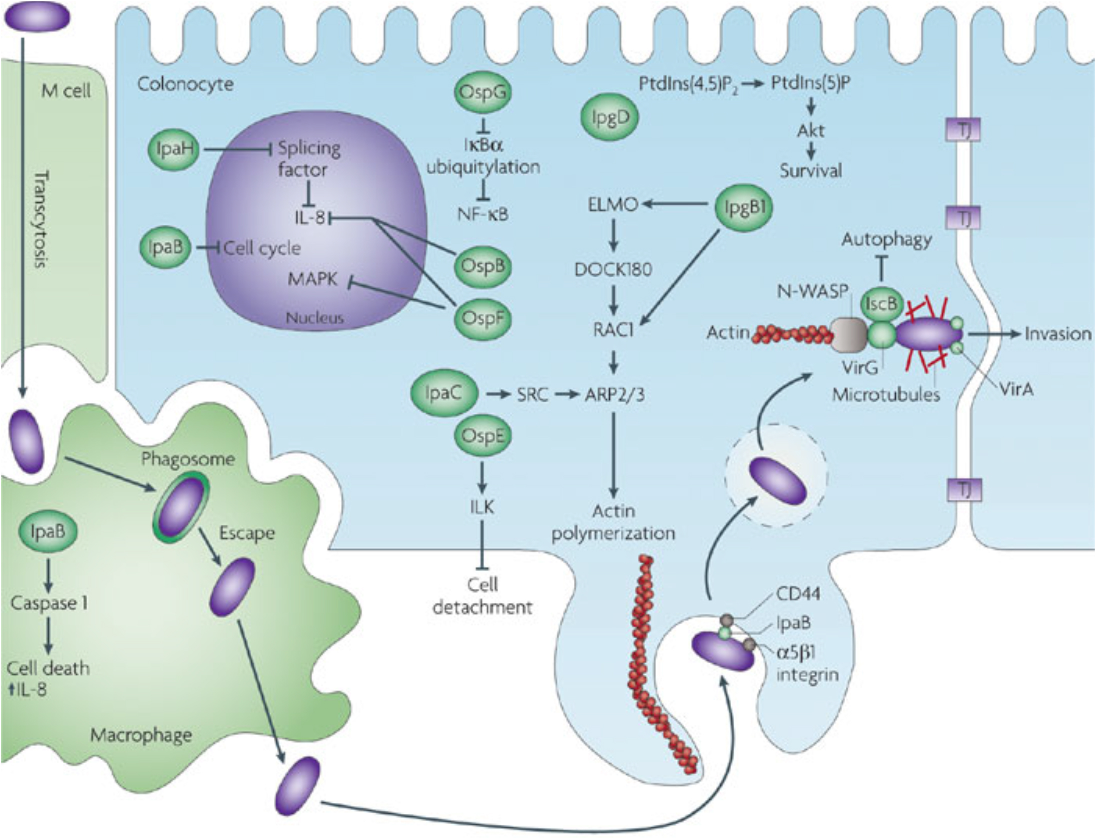
\includegraphics[width=0.95\textwidth]{shigella}
  \caption[Route of infection and intracellular life-cycle of \textit{S. flexneri}.]{\textit{S. flexneri} cross the epithelial barrier of the distal ileum and colon by transcytosis via \acrshort{m-cells}, followed by escape from macrophage digestion. Internalization into epithelial cells from the basolateral side is mediated by trigger mechanism endocytosis. Several bacterial effectors are instrumental in reaching the replicatory niche and ensuring host survival. Adapted from \citet{Croxen2010}.}
  \label{fig:shigella}
\end{figure}

\paragraph{Pathogenesis.}
Main targets of \textit{S. Flexneri} are mucosa of the distal ileum and colon where they enter epithelial cells from the basolateral side. For initial crossing over from the apical side, action of \cgls{m-cells} at Peyer's patches is exploited. These specialized enterocytes constantly sample antigens from the gut lumen and pass them to intraepithelially located dendritic cells and lymphocytes. Upon uptake by basolaterally located macrophages, \textit{S. Flexneri} survive digestive action of the phagosomal vacuole by disrupting the surrounding membrane and initiating host-cell apoptosis, mediated by the bacterial effector protein \acrdbl{ipa}[B], capable of acting on a caspase 1 regulated apoptotic pathway (see figure \ref{fig:shigella}). The bacteria are subsequently released into the sub-mucosa, where they induce phagocytosis by normal epithelial cells via trigger mechanism (see section \ref{trigger-mechanism}).

Initial contact between pathogen and target host cell is mediated by cellular \textalpha\textsubscript{5}\textbeta\textsubscript{1} integrins and binding of \acrdbl{ipa}[B] to CD44 receptors may initiate first actin rearrangements, preparing the cell for uptake. Subsequent injection of at least 6 effector proteins into the epithelial cytosol through the \cgls{t3ss} triggers engulfment of the bacterium in an actin dependent process, involving the small \acrshort{gtp}[ases] \cgls{rac-1} and \cgls{cdc-42}, which recruit the actin nucleation complex \cgls{arp23}. \Acrdbl{ipa}[C], a component of the translocation complex, is involved in stimulating \cgls{rac-1} and \cgls{cdc-42} \acrshort{gtp}[ase] activity through an unknown mechanism and the secreted effector proteins \acrdbl{ipg}[B1], \acrdbl{ipg}[B2], \acrdbl{ipg}[D] and \acrdbl{ipa}[A] facilitate actin polymerization. \acrdbl{ipg}[D], an inositol phosphate phosphatase, catalyzes the hydrolysis of \acrshort{pi45p2} to \acrshort{pi5p} which promotes disassociation of cytoskeleton and membrane, increasing actin availability and making the plasma membrane more susceptibility to manipulation. The mechanism of action of \acrdbl{ipg}[B2] remains to be resolved, while \acrdbl{ipg}[B1] is assumed to mimic activated \acrrev{rho-g}, a small \acrshort{gtp}[ase], located upstream in the signaling pathway of \cgls{rac-1}. Finally, binding of \acrdbl{ipa}[A] to vinculin induces depolymerization of actin, which is assumed to be important for closing of the phagocytic cup.

The resulting phagocytic vacuole has to be escaped before maturation progresses, which is accomplished in a non-acid dependent fashion, by the translocator proteins \acrdbl{ipa}[B], \acrdbl{ipa}[C] and \acrdbl{ipa}[D] via membrane lysis. With release into the epithelial cytosol, the replicatory niche of \textit{S. Flexneri} is reached. Actin mediated intracellular motility enables intercellular dissemination (see section \ref{actin-motility}) and targeting of epithelial tight junctions initiates break-down of the epithelial barrier, providing more pathogens with access to the basolateral side of the gut lining.

\cGls{abm}, is driven by activity of two bacterial proteins. \acrdbl{vir}[A] is secreted at the forward facing end of the rod shaped bacilli, which promotes degradation of tubulin structures and therefore clearing a path through the dense network of microtubules and surface bound \acrdbl{ics}[A], also referred to as \acrdbl{vir}[G], facilitates actin polymerization at the opposite end. Both \cgls{arp23} and \cgls{n-wasp} are involved in actin nucleation, the directed nature of which provides the driving force for locomotion.

In order to maintain their intracellular niche, Shigellae have evolved several strategies. Autophagy is inhibited by IscB (see section \ref{autophagy}) and via the previously mentioned phosphatase action of \acrdbl{ipg}[D], cellular Akt proteins are activated which regulate cell survival and inhibit apoptosis. Furthermore, \acrdbl{ipa}[D] interacts with cell cycle regulatory protein MAD2L2, mediating cell cycle arrest. Together with \acrshort{osp}[E] (\acrlong{osp} E) action on \cgls{ilk}, downregulating cell detachment, this prevents turnover of epithelial cells. Inflammatory response is muddled by a combination of at least four bacterial effectors. Cytoplasmically acting \acrshort{osp}[G] inhibits \cgls{nf-kb}, while nuclearly located \acrdbl{ipa}[H] and \acrshort{osp}[B] reduce \cgls{il-8}. Adding to that, \acrshort{osp}[F] dephosphorylates \cglspl{mapk} that are required for transcription of genes of the \cgls{nf-kb} pathway.

\paragraph{Epidemiology.}
Estimates by the \cgls{who} peg the disease burden caused by \textit{Shigella} \acrshort{spp} at 80 million annual cases worldwide, leading to 700000 deaths. Developing countries are disproportionately affected, representing 99\% of all cases, as are children less than 5 years old, accounting for 70\% of cases and 60\% of deaths. In developed countries, incidence rates of 1--2 per 100000 population are typical and Shigellae are common causes of Traveler's diarrhea.

The predominant route of transmission is fecal--oral, highlighting the importance of sanitary precautions for infection control. Proper treatment of fecal matter is important for preventing contamination of drinking water and inhibiting spreading by disease vectors such as house flies. During acute phases, diseased individuals excrete pathogens in large numbers and as few as 100--200 organisms are sufficient of causing a new infection.

\section{Select Viral Pathogens}

In addition to the previous 5 bacterial pathogens, 3 viruses were selected for study within the InfectX \cgls{rtd} project by SystemsX. This section shortly describes each pathogen in terms of physical features, pathogenesis, epidemiology and diseases caused in humans. For each section, a chapter of \citet{Craighead2000} serves as basis.

\subsection{Adenoviruses}
The family \textit{Adenoviridae} encompasses 5 genera of non-enveloped, medium sized (\SI{90}{\nano\meter} diameter) viruses, capable of infecting a broad range of vertebrate hosts. The capsid is of $T=25$ icosahedral symmetry, composed of 720 hexons arranged as 240 trimers which form the triangular facets and 12 penton capsomeres located at the vertices. A homotrimeric fiber glycoprotein protrudes from each vertex, attached to the penton base via interactions of its N-terminal domains and ending in a globular, C-terminal knob. The genome is present as double stranded \cgls{dna} (Baltimore group I), is non-segmented, linear, 35--\SI{35}{\kilobase} long and encodes 40 proteins.

Adenoviruses were first isolated from human adenoid tissue cultures by Rowe in 1953 and their study led to the discovery of alternative splicing in 1977, a commonly encountered phenomenon among eukaryotes. Currently, 57 serovars are recognized as pathogenic towards humans, all belong to the genus \textit{Mastadenovirus} and are classified into 6 species, labeled A through G. The following sections are mostly concerned with \textit{Human adenovirus C} \citep{Lenaerts2008}.

\paragraph{Diseases.}
In immunocompetent individuals, adenoviruses seldom cause more than transient disease with many infections even occurring subclinically and fatal outcome being very uncommon. Symptomatic cases usually manifest as respiratory tract infections or conjunctivitis and less frequently as hemorrhagic cystitis, nephritis or gastroenteritis. Infections of the oropharynx can spread to the lower respiratory tract, causing bronchitis, bronchiolitis or pneumonia, which can become chronic, leading to desquamated epithelial tissue and long-term damage to the respiratory mucosa. Heart failure and central nervous system involvement can occur in severe cases. Ocular infections range from mild, short-term follicular conjunctivitis to highly contagious keratoconjunctivitis with possible long-term damage to the cornea. \textit{Human adenovirus C} serotypes are mostly associated with respiratory diseases but have also been implicated in eye infections.

Invasive forms of disease are mostly limited to immunocompromised individuals, including transplant recipients, \cgls{hiv} infected, hereditary immunodeficient and cancer patients subject to chemotherapy. In addition to the lungs, a wide variety of organs has been reported to be affected, such as partoid glands, liver, gall bladder, colon, brain and kidney and pathological changes range from perivascular cuffing to parenchymal necrosis.

\begin{figure}
  \centering
  \includegraphics[width=0.95\textwidth]{adenovirus}
  \caption[Molecular mechanisms of adenovirus infection.]{Schematic representation of molecular mechanisms for cell entry and genome replication in adenovirus infection. Formation of the endocytic vesicle is mediated by viral fiber proteins interacting with cellular receptors that in turn recruit clathrin. The \cgls{ccp} is pinched off by membrane scission proteins dynamin-1 and dynamin-2, leading to release of a cytosolic \acrshort{ccv} (A). The adenoviral genome is replicated via a mechanism described as \cgls{dna} strand displacement replication whereby single stranded \cgls{dna} is synthesized from the viral template in a protein primed fashion, which in turn is copied into double strand \cgls{dna}. Figures adapted from \citet{Hulo2011}.}
  \label{fig:adenovirus}
\end{figure}

\paragraph{Pathogenesis.}
Initial attachment of virions is mediated by interactions between the globular knobs of viral fiber proteins and target cell \acrrevpl{car}. In \textit{Human adenovirus C} infections, cellular heparan sulfate proteoglycans serve as additional attachment factors, reinforcing adhesion. Subsequent binding of penton bases to \textalpha,\textbeta-integrin receptors induces clathrin-mediated endocytosis and leads to loss of viral fiber proteins (see figure \ref{fig:adenovirus}, A).

The adenoviral replication cycle is divided into early (E) and late stages (L), with each seeing expression of a typical set of genes. Upon engulfment by the host cell and triggered by endosomal acidification, hexon bound protein VI disassociates from the capsid structure and induces lysis of the endosomal membrane. The remainder of the now cytosolic virion is shuttled to the nucleus by microtubular transport where viral protein IX recruits kinesin thereby procuring capsid disruption.

Nuclear penetration is mediated by core protein VII and occurs at \cglspl{npc}, leading to transcription of early viral genes by host \cgls{rna} polymerase II. The resulting proteins manipulate various cellular processes, such as evasion of host immune response (E3, E19), cell cycle (E1A), apoptosis (E1B and E4), autophagy (E1B) and \cgls{mrna} transport (E4), while also promoting viral \cgls{dna} replication (E2). Modulation if the adaptive immune response is mediated by the \cgls{tap} inhibitor E19, as binding of \cgls{tap} prevents loading of peptides onto \cgls{mhc} class I molecules for display on the cell surface. In order to create an optimal environment for replication, viral protein E1A induces a G1\slash S cell cycle transition which increases the concentration of cellular enzymes involved in \cgls{dna} replication. This, however, also leads to accumulation of cellular p53, participating in apoptosis signaling. Several viral proteins, including E1B 55K and E4 orf6 have been shown to inhibit the apoptotic pathway. E1B 19K is involved in activation of autophagy thereby contributing to the delay or inhibition of apoptosis.

A virally encoded \cgls{dna} polymerase replicates the genome by \cgls{dna} strand displacement in an unusual protein primed fashion involving \cgls{ptp} acting as primer and \cgls{dbp}, stabilizing single stranded \cgls{dna}, as well as several host proteins (figure \ref{fig:adenovirus}, B). With onset of replication, translation of late genes by host \cgls{rna} polymerase II is initiated, leading to the production of structural proteins and proteins required for virion assembly. Encapsidation occurs in the nucleus and progeny virions are released by lysis of the host cell.

\paragraph{Epidemiology.}
Adenoviruses are endemic and ubiquitous, causing an estimated 2--5\% of all respiratory infections. Distribution is worldwide and incidence is higher in the first half of the year. Children are frequently infected as serological studies show that by the age of 5 years some 50\% present antibodies towards the most common species, including \textit{Human adenovirus C}. On the order of 1 in every $10^7$ lymphoid cells in the oropharynx harbor fully assembled latent sate virions, making most humans latent carriers. Transmission can both occur via respiratory droplet or fecal-oral routes and virions are very stable towards chemical and physical agents, surviving for long periods outside their host.

Adenovirus outbreaks are a common cause of pneumonia in militaries, leading to the development of live, oral vaccines in the 1960's by the United States Army. The only supplier, however, ceased production and as of 1999, vaccinations could no longer be administered, resulting in reemerging incidence. In the first 5 years after loss of the vaccine, 110000 cases of febrile respiratory illness were reported, of which an estimated 90\% are considered preventable. By October 2011, new vaccine again was available and and has been administered to new recruits since.

\subsection{Rhinoviruses}
Investigations into the etiological agent of the common cold within the British Common Cold Research Unit led to the discovery of rhinoviruses in 1953. Initially classified as a separate genus of the family \textit{Picornaviridae}, recent genomic evidence led to a revised taxonomy, recognizing three species of rhinoviruses (A through C) as members of the genus \textit{Enterovirus}. Over 100 distinct serotypes have been isolated from humans, 74 belong to species A, 25 to B and the newly identified species C, currently under active study, may encompass an additional 55 types.

Rhinovirus virions are small (\SI{30}{\nano\meter} in diameter), non-enveloped, with a pseudo $T=3$ icosahedral capsid, consisting of 4 different polypeptides (VP1, VP2, VP3 and VP4) surrounding the \cgls{rna} genome. There are 60 copies of each structural protein and VP1--3 face towards the outside and are responsible for antigenic diversity, while VP4 faces inwards and anchors the \cgls{rna} core to the capsid. A canyon formed by VP1 and VP3 serves as receptor binding site. The viral genome consists of monopartite, linear, single stranded, positive sense \cgls{rna}, roughly \SI{7.2}{\kilobase} in length and encodes a single polyprotein, which cleaved by viral proteases yields 11 proteins. Instead of a methylated 5' cap, the \cgls{rna} genome is terminated by a viral protein (VPg) at its 5' end \citep{Jacobs2013}.

\paragraph{Diseases.}
Over half and up to two thirds of all cold-like illnesses are thought to be caused by rhinoviruses. In addition, asymptomatic infections, especially in children are very common with rates among children under 4 years ranging from 12 to 32\%. These surprisingly high numbers may to some extent result from virus persistence in hosts that have recovered in addition to disease that has not broken out. In adults, rates of asymptomatic carriage are significantly lower, reported at 0--2\%.

In immunocompetent individuals, symptomatic disease typically manifests as upper respiratory infection with clinical syndromes associated with common cold, including rhinorrhea, nasal congestion, sore throat, headache and possibly fever and general malaise. Disease is self-limited, incubation periods are between 12 and 72 hours and within 7 to 14 days symptoms wear off. A common complication is acute otitis media, which has been reported to happen in up to 30\% of cases in early childhood. In 41--45\% of investigated middle ear infections, rhinoviruses were detected. Further cavities that are frequently infected are the paranasal sinuses. Nose blowing has been suggested as mechanism for spreading the virus and causing rhinosinusitis.

Initially thought to primarily cause benign upper respiratory infections,  recent data clearly implicates rhinoviruses in more severe lower respiratory infections. Croup, bronchiolitis and \cgls{cap} have been associated with rhinovirus infections and studies have shown that in 12--26\% of cases, rhinoviruses were present. Furthermore, a study of children admitted to \cglspl{icu} with lower respiratory tract infections detected no other pathogens in 49\% of the patients. Immunocompromised individuals are predisposed to contracting more serious forms of disease, with morbidity and mortality comparable to that of pandemic H1N1 influenza.

While not typically associated with cytopathogenic effects on epithelia of the upper respiratory tract, cell damage to lung tissue, especially among children, has been documented. Thus, rhinoviruses are linked to exacerbations of chronic pulmonary diseases such as asthma, chronic obstructive pulmonary disease and cystic fibrosis.

\begin{figure}
  \centering
  \includegraphics[width=0.95\textwidth]{rhinovirus}
  \caption[Capsid structure and genome of rhinoviruses.]{Capsid proteins VP1 through VP4 form a pseudo $T=3$ icosahedral coat, roughly \SI{30}{\nano\meter} in diameter around the \cgls{rna} genome (A), which is monopartite, linear, \SI{7.2}{\kilobase} long and encodes 11 proteins (B). Figures adapted from \citet{Hulo2011}.}
  \label{fig:rhinovirus}
\end{figure}

\paragraph{Pathogenesis.}
Members of rhinovirus species A and B are divided into two group according to their host cell receptors. Members of the major group form interactions with \cgls{icam-1} while minor group types (including serotype 1a) associate with \cglspl{vldlr}. Attachment of species C have very recently been identified as induced by \cgls{cdhr3}. Upon receptor mediated endocytosis, pH dependent conformational changes in capsid structure exposes VP4 which has pore-forming properties and facilitates release of viral genomic material into the cytosol.

Host cell ribosomes readily translate the released positive-sense \cgls{rna} into polyprotein, which is cleaved in \textit{cis} by 2A and 3Cpro, yielding preproteins P1, P2 and P3 (see figure \ref{fig:rhinovirus}. P1 is digested into structural capsid proteins while P2 and P3 are further processed to produce the replication machinery. Viral \cgls{rna}-dependent \cgls{rna} polymerase synthesizes a complementary, negative-sense \cgls{rna} strand, primed by VPg, which in turn serves as template for many copies of the viral genome. These can be both translated into more protein and in a later stage of replication also be packaged into progeny virions. Final cell export is mediated by host-cell membrane lysis.

\paragraph{Epidemiology.}
Despite most infections with rhinoviruses only resulting in mild disease, economic impact both due to health care costs and loss of productivity is considerable. This is primarily owed to the overwhelming prevalence of these pathogens. Respiratory illnesses attributed to rhinoviral infections occur throughout the world and all year round with peak incidences in early fall and spring. Vaccination efforts so far have been futile, mainly because of the large number of serotypes and lack of individual epidemiological data.

Due to acid-sensitivity, fecal-oral infection is unlikely most person-to-person transmission occurs through aerosols and contact spread either direct of via fomites. Extra-host survival times of hours to days have been reported for indoor environments and up to 2 hours on undisturbed skin.

\subsection{Vaccinia}
\textit{Vaccinia virus} is a species within the genus \textit{Orthopoxvirus}, alongside the exceptionally virulent \textit{Variola virus}, the etiological agent of smallpox. Immunological similarities between the two species allows for cross-protection, which coupled with the large discrepancy in pathogenicity presents a fortunate opportunity for artificially inducing acquired immunity. This was recognized by Jenner in 1798, while investigating the zoonosis of \textit{Cowpox virus} and subsequent susceptibility towards contraction of smallpox. The origins of vaccinia are unknown. It has been speculated to have derived from cowpox or smallpox, to be a hybrid of both and of being the prototype orthopoxvirus, as well as descending from an extinct ancestor.

The virions are large and brick shaped, measuring 200 by 250 by \SI{340}{\nano\meter} and exist as both \cgls{mv} and \cgls{ev}. Structurally they are unusually complex. The linear, double-stranded \cgls{dna} genome, roughly \SI{200}{\kilobase} long, is encased in an S-shaped, tube-like nucleocapsid with an outside diameter of \SI{50}{\nano\meter}, a cavity of \SI{10}{\nano\meter} and an overall length of \SI{250}{\nano\meter}. Additionally, 47 viral proteins, of which 16 are involved in early \cgls{mrna} synthesis and 28 have no known enzymatic function, are packed into a core structure. The core wall consists of two layers, the palisade (outer) layer which is \SI{17}{\nano\meter} thick and an inner smooth layer, measuring \SI{8}{\nano\meter} across. Centered on the top and bottom faces, two proteinaceous lateral bodies separate core from the surface membrane, forming the virion core into a biconcave disc with dumbbell shaped vertical cross sections. The lipidic surface membrane also consist of two layers, the outermost measuring \SI{9}{\nano\meter} and the innermost domain is \SI{5}{\nano\meter} thick. \cGls{ev} virions are additionally wrapped in a membrane derived from Golgi cisternae \citep{Marennikova2005,Condit2006}.

\paragraph{Diseases.}
While infection with variola causes severe disease manifesting in skin lesions covering the whole body, accompanied by 20--40\% mortality rates, the closely related \textit{Vaccinia virus} is far less invasive. Virulence of the latter pathogen is so low that it has been routinely used as live vaccine against the former. Owing to the massive effort put into the worldwide fight against smallpox led by the \cgls{who} in the late 1960's and throughout the 1970's, the disease was found to be eliminated by 1980. At the center of the smallpox eradication program was the administration of freeze-dried, calf lymph derived vaccinia with a bifurcated needle, by multiple pricking of the skin. Towards the end of the initiative, 200 million vaccinations were performed annually.

The predominant reaction to vaccinia inoculation is localized, self-limited disease. After an incubation period of of 3--4 days, a papule with a sunken center develops at the site of infection, accompanied by erythema and swelling. Over the following days the papule increases in size and liquid begins to accumulate within. Fever may develop around days 7--10, possibly followed by malaise, headache and anorexia. Local lymphadenopathy is frequently encountered and days 8--10 typically mark the beginning of involution of the papule, which subsequently drys out and forms a scab.

Of great concern for routine vaccination procedures are complications which inevitably occur in a small numbers. Atypical side effects develop in roughly 1 per mill of cases and potentially life threatening reactions usually manifest as neurological (477.4 cases and 47.0 fatalities per 1 million) or cutaneous disease (278.4 cases and 0.2 fatalities per 1 million). Predisposing conditions for central nervous system involvement are not known and despite decades of inquiry into this pathology, it remains poorly understood. Symptoms range from febrile seizures to severe encephalitis, but so far no  neuropathological characteristics have been identified. Complications affecting the skin and mucous membranes are classified as progressive vaccinia, eczema vaccinatum and generalized vaccinia and disease severity decreases in this order. Predisposing conditions for progressive and generalized vaccinia are immunodeficiencies while a history of eczema is a risk factor for eczema vaccinatum.

\begin{figure}[t]
  \centering
  \includegraphics[width=0.75\textwidth]{vaccinia}
  \caption[Replication cycle of \textit{Vaccinia viruses} for both intracellular mature and extracellular enveloped virions.]{Replication cycle of \textit{Vaccinia viruses} for both \acrfull{mv} and \acrfull{ev}. Cell entry is either macropinocytic or proceeds via membrane fusion, followed by uncoating and replication. Host exit proceeds by either lytic or exocytic mechanisms. Figure adapted from \citet{Hulo2011}.}
  \label{fig:vaccinia}
\end{figure}

\paragraph{Pathogenesis.}
Initial attachement is mediated by interaction between viral proteins and cellular heparan sulfate chains. For cell entry, various strategies have been reported, dependent on the virus strain. WR strains induce macro\-pinocytosis and proteins A25\slash A26 act as fusion suppressors that only cease action under acidic conditions encountered in maturing endosomes, while other strains, such as Copenhagen, present no A25\slash A26 on their outer membrane and fuse directly with the target. Due to the additional membrane of \cglspl{ev}, an alternative entry mechanism is required. In a currently not well understood fashion, the outer membrane is lost by non-fusogenic disruption, followed by fusion of the inner virion membrane. All pathways lead to cytosolic localization of virions devoid of their envelope (see figure \ref{fig:vaccinia}).

Members of the \textit{Poxviridae} family are special among Baltimore group I viruses in that their genome encodes all necessary replicatory proteins, allowing for cytosolic localization. Replication is temporally tightly regulated and consists of distinct phases (early, intermediate and late gene expression). Each class of genes encodes factors capable of initiating the succeeding stage, providing transcription level regulation. Uncoating of the core structure releases early proteins, including \cgls{rna} polymerases and enzymes for \cgls{mrna} processing which start transcribing early genes. At least 50 different products, such as \cgls{dna} replicatory enzymes, additional \cgls{rna} polymerase, \cgls{mrna} processing machinery, host defense molecules and intermediate gene transcription factors, have been identified and account for 25\% of the viral coding capacity. Early gene transcripts are detectable 20 minutes after cell entry and reach their productive peak within 100 minutes of infection.

Expression of intermediate genes is initiated by accumulation of intermediate  transcription factors and the onset of \cgls{dna} replication. Only 7 products of this phase are known, which functionally are mostly concerned with host defense, \cgls{dna}\slash \cgls{rna} metabolism and commencement of the final phase. Beginning 100 minutes after infection, intermediate gene transcription reaches its peak at 120 minutes and is thereafter superseded by late gene transcription, beginning 140 minutes after cell entry. Products of the final phase comprise a large number of genes (up to 75\% of the vaccinia genome) and include enzymes needed for initiating replication (\cgls{rna} polymerase and modification proteins), early transcription factors and structural proteins, as well as virion assembly machinery.

\cgls{dna} replication not only serves for progeny virions, but also to increase the concentration of templates used for gene expression. Both \cgls{dna} synthesis and virion assembly occur within factories, readily visualized by electron microscopy as electron dense cytoplasmic inclusion bodies. Owing to the complex virion structure \cgls{dna} packaging and virion assembly is an involved procedure with is incompletely understood.

\paragraph{Epidemiology.}
It is unknown if a natural reservoir of vaccinia exists. It has been speculated that the virus is maintained only within research laboratories and vaccination production facilities, while others have implicated some rodent species as possible reservoir hosts. Small scale zoonotic outbreaks of vaccinia have been documented in Brazil and it was initially suspected that these were linked to vaccine that had escaped into the environment. Recent phylogenetic studies however were able to rule out this explanation but were unable to shed further light into underlying epidemiological mechanisms.

While transmission from vaccinees to unvaccinated individuals is rare, direct contact transmission is possible and such occurrences have been documented. Special care has to be taken to avoid direct contact between recently vaccinated and individuals predisposed towards developing complications.

\section{RNA Interference}
First described only two decades ago, regulation of gene expression by short strands of \cgls{rna} has become an indispensable tool to both experimental biology and bioinformatics. Recognizing the importance of applications made possible by this discovery, the 2006 Nobel prize in Physiology or Medicine was awarded to Fire and Mello who studied \acrlong{rnai} in the nematode worm \textit{Caenorhabditis elegans} and published their findings in 1998. Building on studies by Guo and Kemphues, who showed that sense \cgls{rna}, as well as antisense \cgls{rna} was capable of suppressing gene expression, Fire, Mello and coworkers found that double stranded \cgls{rna} was at least ten-fold more effective as silencing agent than individual single stranded fragments. Further investigations showed that several gene regulatory processes, previously thought to be unrelated, were in fact manifestations of \cgls{rna} interference and that the underlying mechanism was conserved in many, if not most, eukaryotic organisms \citep{Hannon2002}.

The \cgls{rnai} pathway can take as input two separate types of \cgls{rna} molecules, \cgls{mirna} and \cgls{sirna}, of differing origins. While \cglspl{mirna} are endogenous and purposively employed in post-transcriptional regulation of gene expression, \cglspl{sirna} are exogenous synthetic or viral inducers of gene suppression, in which case, \acrlong{rnai} can be viewed as an immune response to foreign genetic material. Parsimony-based phylogenetic analysis of involved genes suggests that the key components to an \cgls{rnai} system were already present in the last common ancestor of eukaryotes and were subsequently lost or extensively simplified in some protists. The original function of \cgls{rnai} is hypothesized to be that of a defense mechanism against genomic parasites as indicated by the extent of its conservation, whereas \cgls{mirna}-directed silencing most probably was introduced at a later point in evolution \citep{Cerutti2006}.

\subsection{Molecular Mechanism\footnote{This section is based on the three review articles by \citet{Wilson2013}, \citet{Kim2007} and \citet{Carthew2009}.}}
\acrlong{rnai} refers to three separate mechanisms for regulation of gene expression by small \cglspl{rna}, as visualized by figure \ref{fig:rnai}. While \cglspl{sirna} are involved both in transcriptional and post-transcriptional gene silencing, the \cgls{mirna} pathway is focused on translational repression. The severity of action on the targeted genes once again highlights the differing purposes of the \cgls{sirna} and \cgls{mirna} pathways, one tasked with inhibitory and the other with regulatory measures.

\begin{figure}[t]
  \centering
  \includegraphics[width=0.7\textwidth]{rnai}
  \caption[The three major pathways of \acrlong{rnai}.]{\acrlong{rnai} comprises of three distinct mechanisms that yield control over gene expression. Exogenous double-stranded \cgls{rna} are processed into \cgls{sirna} fragments that both act inside the nucleus as transcriptional silencing agents and in the cytoplasm, post-transcriptionally cleaving \cgls{mrna} strands. Endogenous \cgls{mirna} is synthesized by \cgls{rna} polymerase, originates from the nucleus in processed form and mediates milder translational repression Figure adapted from \citet{Kim2007}.}
  \label{fig:rnai}
\end{figure}

\paragraph{Translational repression by \cgls{mirna}.}
The biogenesis of \cgls{mirna} occurs in the nucleus and is initiated by \cgls{rna} polymerase II transcription of long (\textgreater \SI{1000}{\nucleotide}) \cgls{pri-mirna} segments, characterized by double-stranded hairpin loops with single-stranded 5'- and 3'-terminal overhangs which are poly\-adenylated and capped. Subsequent processing by the microprocessor complex consisting of the \acrrev{rnase} III family enzyme Drosha and \acrrev{dgcr8} yields \tilde 60--\SI{70}{\nucleotide} stem-loop structured \cgls{pre-mirna} fragments. \cgls{dgcr8} recognizes \cglspl{pri-mirna} by the junction of stem and single-stranded overhang and helps positioning the substrate for endonucleolytic cleavage by Drosha at a site \tilde \SI{11}{\nucleotide} from the junction. Nuclear export is mediated by the transport facilitator exportin-5 and is \acrshort{ran}-\acrshort{gtp} dependent.

In the cytoplasm, \cglspl{pri-mirna} are targeted by Dicer and the associated \cgls{dsrna} binding proteins \acrrev{trbp} and \acrrev{pact}. These process their substrate into 21--\SI{25}{\nucleotide} \cgls{dsrna} strands with \SI{2}{\nucleotide} overhangs at the 3' termini and phosphate groups at each of the recessed 5' ends. The mature \cglspl{mirna} are loaded onto \acrrev{ago} by Dicer, which leads to the formation of \cgls{risc}. Concomitantly with \cgls{risc}-loading, one of the two \cgls{rna} stands is selected as guide strand whereas its complement (the passenger strand) is ejected and degraded. Thermodynamic asymmetry between the two strands is exploited in this step and the strand with the less stable 5' end is preferred. As opposed to strand separation in \cglspl{sirna}, the passenger strand is not cleaved but rather unwound by helicase activity, facilitated by imperfect sequence alignment.

Finally, active \cgls{risc}, exposing the \cgls{ago}-bound guide strand, interacts with the 3' untranslated region of \cgls{mrna} targets and directs translational repression and \cgls{mrna} degradation. Sequence homology between \cgls{mrna} and the \cgls{mirna} seed sequence (the first 2--6 or 2--\SI{8}{\nucleotide} from the 5' end) is critical while mismatched nucleotides towards the 3' end of the \cgls{mirna} are readily tolerated. The extent of base-pairing influences the subsequent mechanism of silencing, ranging from direct target cleavage (perfect match) over deadenylation (followed by degradation) to nonendonucleolytic translational repression (imperfect match).

\paragraph{Post-transcriptional gene silencing by \cgls{sirna}.}
Precursors to \cgls{sirna} are long, linear, perfectly base-paired double stranded sequences of \cgls{rna}, typically of exogenous origin either introduced directly into the cytoplasm, or taken up from the environment. A complex consisting of Dicer and several \cgls{rna}-binding proteins are responsible for trimming down \cgls{dsrna} fragments to the appropriate size for loading onto \cgls{ago}[2]. Of the four \cgls{ago} family members in humans, capable of associating with \cgls{mirna}, only \cgls{ago}[2] seems to be involved with \cgls{sirna}. Furthermore, \cgls{ago}[2] is the only mammalian \acrlong{ago} member bearing endonucleolytic functionality and therefore capable of directly cleaving targeted \cgls{mrna}.

Strand selection is again based on differences in stability of base-pairing at the 5' termini with the weaker interacting end being favored as guide strand. Accuracy of discrimination can be low, leading to incorporation of both strands with equal frequency. In contrast to \cgls{mirna} loading, the passenger strand is not merely separated but directly cleaved by \cgls{ago}[2] and the differing treatment seems to only depend on perfect strand complementarity given in \cgls{sirna} and absent in \cgls{mirna}. Upon \cgls{rna} incorporation, \cgls{risc} is formed and activated by cleavage of the passenger strand. The 3' guide strand end is bound by the \acrshort{ago} protein's \cgls{paz}, while the 5' end interacts with \cgls{mid}, closely located to the catalytic \cgls{rnase} H-like \cgls{piwi}.

Post-transcriptional gene silencing is accomplished by endonucleolysis of perfectly matching \cgls{mrna} precisely at the phosphodiester linkage between bases 10 and 11 relative to the 5' terminus of the \cgls{sirna} guide strand. Following cleavage, the target disociates, freeing \cgls{risc} for further catalysis, and the \cgls{mrna} fragments are degraded by cellular exonucleases. Imperfectly matched \cgls{mrna} may be targeted, much like it is the case with \cgls{mirna}, leading to \cgls{sirna} off-target effects which are of great practical importance.

\paragraph{Transcriptional gene silencing by \cgls{sirna}.}
In addition to post transcriptional action of \cgls{sirna}, nuclear inhibition of gene transcription has been described in many eukaryotes. Diced \cgls{sirna} fragments are transported into the nucleus where they are assembled with a group of proteins, including \cgls{ago}[1], to form \cgls{rits}. Currently only incompletely understood, the \cgls{sirna} guide strand is thought to recognize \cgls{rna} transcripts as the emerge from \cgls{rna} polymerase II, followed by recruitment of factors that enable covalent modifications of nearby histones. Methylation of lysines 9 and 27 in H3 by histone methyltransferases leads to chromatin compaction and heterochromatin formation. \cGls{rits} has also been shown to induce direct methylation of \cgls{dna}, repressing gene expression even further.

Contributing to the potency of \acrlong{rnai}, engagement of \cgls{rits} with nascent transcripts activates the \cgls{rdrc}, capable of generating secondary \cgls{sirna} fragments and therefore amplifying silencing capabilities. The role of this reinforcement mechanism has been firmly established in many eukaryotic \cgls{rnai} systems with the notable exceptions of vertebrates and insects. Whether a similar system exists in these organisms remains an open question.

\subsection{Biological Function}
The mechanisms of \acrlong{rnai} have most probably evolved in order to protect against foreign genetic material such as parasitic \cgls{dna} sequences or viral \cgls{rna}. Transposable elements (transposons) are \cgls{dna} sequences that are mobile within the genome, can make up a significant fraction of eukaryotic genomes and are typically considered non-coding. Transposition is mediated by transposases, enzymes often encoded within the transposons themselves, that act on specific sequences at the transposon ends and cause unspecific insertion into new target sites. Retrotransposons move via an \cgls{rna} intermediate which is reverse transcribed to \cgls{dna} and inserted, while \cgls{dna} transposons employ a cut and paste mechanism. Retroviruses therefore can be viewed as transposons and in general, transposable elements are a form of selfish \cgls{dna} that often incur deleterious effects.

\cgls{rnai} is an important regulatory force to transposon activity, both by processing transcripts of retrotransposons, thereby reducing their concentration and eliciting epigenetic modifications, as well as transcriptional inhibition via heterochromatin formation. The importance of keeping transposable elements in check is highlighted by their prevalence, with roughly half of the human genome being thought to derive thereof.

Antiviral mechanisms are particularly important in organisms lacking an adaptive immune system as found in vertebrates and exploiting the orthogonality of most genomic systems to double-stranded \cgls{rna} puts \acrlong{rnai} in a powerful position. Corroborating this notion is the observation that, in \textit{Drosophila melanogaster}, three key proteins of the \cgls{rnai} pathway (Dicer-2, \cgls{ago}[2] and R2D2, a protein involved in \cgls{risc} loading) are among the top 3\% in terms of genetic instability. Furthermore, \cgls{mirna} pathway paralogs to these three genes (Dicer-1, \cgls{ago}[1] and R3D1), not being involved in immune response, evolve at a much slower rate \citep{Obbard2009}.

Although small \cgls{rna}-guided, \cgls{ago}-dependent up-regulation of gene expression (termed \acrlong{rnaa} or \acrshort{rnaa}) has been described, most regulation of gene expression by \cgls{mirna} is of inhibitory nature. This widespread mechanism, consisting of \textgreater 1000 \cgls{mirna} sequences (as much as 5\% of the human genome) controls at least 30\% of human genes and is responsible for vital processes including cell growth, tissue differentiation and cell proliferation.

\subsection{Applications}
In \textit{C. elegans}, \acrlong{rnai} is especially powerful, making it a popular model organism for \cgls{rnai}. Not only is delivery efficiently possible simply by feeding the nematodes with bacteria such as \textit{E. coli} that carry the desired \cgls{dsrna}, but the resulting gene silencing effects are hereditary. Moreover, \cgls{rnai} response is not stoichiometric but catalytic, is amplified in a feedback loop and in many organisms, systemic spread has been documented.

The initial burst of excitement surrounding possible applications was somewhat moderated by difficulties in applying \cgls{rnai} to mammalian systems. At first it seemed impossible to use this technology in somatic cells as the introduction of \cgls{dsrna} is typically met with overwhelming non-specific responses, including  \acrrev{pkr}, which leads to arrest of translation and apoptosis. This issue was shown to be overcome by exclusively using \cglspl{sirna} duplexes of 21--\SI{23}{\nucleotide} with 2-nt 3' overhangs that mimic Dicer products and are too short for inducing \cgls{pkr}. Mammalian \cgls{rnai} response, however is transient, lacking amplification and spreading mechanisms documented in other organisms (mainly plants and worms) and delivery, especially in vivo remains problematic. A further issue that continues to be an actively researched area of interest is that of \cgls{ote}, which considerably complicate the interpretation of phenotypic data.

\paragraph{Gene knockdown studies.}
Large-scale \cgls{lof} and modifier or synthetic lethality screens are readily possible by means of \cgls{rnai} based \cgls{hts}. Such experiments usually proceed by arraying libraries of gene specific \cglspl{sirna} onto microtiter plates (96 and 384 well formats are common), followed by the addition of liquid cell cultures. After an appropriate transfection time, the cells may be subjected to an additional treatment, such as exposure to drugs or pathogens (modifier screen) or \cgls{lof} phenotypes can be investigated directly. Assay readout is performed via optical measurements such as detection of fluorescence or luminescence signals or by microscopic imaging (confocal or wide-field).

Transcriptional reporters, fluorescent dyes that detect enzymatic activity and protein-modification specific antibodies have been employed in plate reader-based investigations which yield a single numerical readout per well. This quantitative approach is contrasted with microscopy based assay read-outs that are able to capture spatial information on antibody stained proteins, fluorescently labeled cellular structures and \cgls{gfp} expression, yielding much more data per well. Significant challenges incurred by automated high-content imaging have successfully been addressed by computational image analysis software.

A multitude of technical and biological noise sources contribute to serious problems in interpretability and comparability of observed data. Common to all \cgls{hts} approaches, errors arise from difficulties guaranteeing equal conditions in a large number of parallel experiments. Liquid dispensing errors, temporal disparities caused by bottleneck resources such as imaging equipment and spatial discrepancies, for example inhomogeneous temperature distribution over the plate or liquid evaporation in border wells, are only a few issues that come to mind. Biological sources of error include \cglspl{ote}, varying potency of reagents (both the knockdown strength and time required to achieve optimal knockdown) and obscuration of assay phenotype by knockdown phenotype (e.g. cell death). Furthermore, incorrect gene models lead to errors in library design and detection may be hampered by weak phenotypes. Replicates, although expensive in large-scale experiments and control wells embedded in every assay plate are indispensable measures in order to assess reproducibility of the data \citep{Echeverri2006,Perrimon2007}.

Despite being a young technology, \acrlong{rnai} has already proven itself as an invaluable tool and has yielded many insights with significant impact on various fields. A review by \citet{Mohr2010} lists some of these findings which lead to refined understanding of cell proliferations, cancer biology, cell cycle regulation, mitochondrial diseases, signal transduction, \cgls{rna} biology and pathogen response. 

\paragraph{Biotechnological applications.}
Intercellular, systemic spread of \cgls{rnai} response in plants and even its heredity over several generations have been documented and it comes as no surprise that the technology is investigated for possible utilization in crop improvement. Removal of plant endotoxins by targeting genes of toxin biosynthesis has been accomplished, leading to the production of decaffeinated coffee plants (knockdown of theobromine synthase), tobacco with reduced concentration of carcinogenic compounds (inhibition of nicotine demethylase activity) and edible cotton seeds (reduction of delta-cadinene synthase leads to low levels of gossypol, a toxic terpenoid), which are naturally rich in dietary protein.

In addition to investigations with consumer health in mind, improvements in environmental resistance have been studied in many organisms. Susceptibility to bacterial and viral pathogen infection has been reduced in rice, bean, barley and lemon, while fungal resistance has been increased in potato, tobacco and wheat. Successful \cgls{rnai} application as insecticide has been shown in cotton and maize and even improved resistance to parasitic weeds could be demonstrated in transgenic tomato plants. Despite these achievements, concerns over environmental issues and adverse health effects have so far prevented \cgls{rnai} based genetic modifications from exiting experimental stages \citep{Saurabh2014}.

\begin{table}
  \centering
  \caption[A selection of \acrfull{rnai} based drugs in clinical trials.]{A non exhaustive list of \cgls{rnai} based drugs that currently are in clinical trials. The data was obtained from the clinicaltrials.gov database \citep{McCray2000}.}
  \label{tab:rnai-clinical}
  \footnotesize
  \begin{tabular}{L{0.14\linewidth}L{0.24\linewidth}L{0.24\linewidth}L{0.18\linewidth}}
    Company &
      Disease &
      Delivery system &
      Status \\
    \hline 
    Alnylam &
      Transthyretin-Mediated Amyloidosis &
      \acrshort{sirna}–\acrshort{galnac} conjugate &
      Phase III recruiting \\
    Alnylam &
      Antitrypsin Deficiency Liver Disease &
      Liposome &
      Phase II recruiting \\
    Alnylam &
      Acute Intermittent Porphyria &
      \acrshort{sirna}–\acrshort{galnac} conjugate &
      Phase I recruiting \\
    Silenseed &
      Advanced pancreatic cancer &
      Polymer (\acrshort{loder}) &
      Phase III planned \\
    Sylentis &
      Dry eye syndrome &
      Naked \acrshort{sirna} &
      Phase II completed \\
    Sylentis &
      Open angle glaucoma &
      Naked \acrshort{sirna} &
      Phase II recruiting \\
    Tacere &
      Chronic hepatitis C &
      \Acrlong{aav}\glslocalreset{aav} vector &
      Phase II recruiting \\
    Tekmira  &
      Advanced Hepa\-to\-cellular Carcinoma &
      Liposome &
      Phase II recruiting \\
      \hline
  \end{tabular}
\end{table}

\paragraph{Therapeutic potential.}
Great promise lies in therapeutic application of \cgls{rnai} as theoretically, any gene can be targeted, yielding unparalleled flexibility not encountered with typical small molecule drugs. An initial obstacle to harnessing this power in humans is the issue of delivery. Systemic spread of naked \cglspl{sirna} is hampered by kidney filtration, phagocytic uptake and degradation by serum \cglspl{rnase}. Movement across capillary walls is not readily possible for molecules larger than \SI{5}{\nano\meter} and phagocytes patrol the extracellular matrix, ingesting foreign genetic material. Furthermore, polyanionic macromolecules do not easily penetrate hydrophobic cellular membranes.

Topical or local administration offers advantages, including increased bioavailability and reduced side effects and is therefore preferred for treatment of eye, skin and mucosal diseases, as well as localized tumors. If targets are not localized or difficult to reach, injection into the bloodstream may provide a mode of systemic application. Chemical modification of the \cgls{rna} backbone (2'-O-methylation or 2'-fluorination of ribose) has been shown to provide resistance to \cgls{rnase} and covalent attachment to cholesterol promotes cellular uptake. Encapsulation of \cgls{sirna} in liposomes and cationic polymers are further proven techniques for improving extracellular stability, stimulate endocytosis and facilitate endosomal escape.

Some sort of target selectivity is desirable on order to avoid high dosages, associated concerns of toxicity and potential \cglspl{ote} in non-target tissue. Coupling of \cgls{sirna} reagents to antibodies specific for \cgls{hiv} envelope glycoproteins has been successfully employed for selectively entering infected cells, while aptamers (oligonucleotides specifically engineered for binding a given target), carrying \cglspl{sirna} have also been shown to be capable homing mechanisms.

Viral delivery of of \cgls{rnai} inducing agents presents an alternative technique to the above and in case of retroviral transport vessels, \cglspl{shrna} that are reverse transcribed and integrated into the host genome, provide stable expression and prolonged \cgls{rnai} activity. Adenoviral and \cgls{aav} vectors have also been employed, resulting in a more transient response. While health concerns associated with perpetuity of gene therapy no longer apply, repeated administrations may prove problematic, triggering strong immune response and thereby limiting therapeutic potential.

Currently, multiple \cgls{sirna} based therapeutics are in clinical trials, including stage III studies (see table \ref{tab:rnai-clinical}). Due to the unprecedented pace at which \cgls{rnai} technology went from discovery to development of applications, much uncertainty remains surrounding long term effects of exposure to such drugs. Chronic diseases including hepatitis C or \cgls{hiv} infections require life-long treatments and consequences of repetitively triggering \cgls{rnai} response has not been thoroughly studied (unwanted changes to chromatin structure for example, are one area of concern). Apart from safety issues, several implementation aspects require further study. While neurodegenerative diseases have successfully been treated in mouse models via direct injection into the brain, this is not easily feasible in human patients and currently no delivery vehicle capable of crossing the blood-brain barrier. \citep{Kim2007,Whitehead2009},

%\chapter{Mathematical Background}

Modeling the relationship among variables is one of the most important applications of statistical theory. The study of regression analysis (and the closely related notion of correlation) started to form towards the end of the 19th century with Sir Francis Galton's study of height heredity in humans and his observation of regression towards the mean. Over the next few years, Udny Yule and Karl Pearson cast the developed concepts into precise mathematical formulation, in turn building on work performed by Adrien-Marie Legendre and Carl Friedrich Gauss who developed the method of least squares almost a century earlier \citep{Allen1997}.

A multiple linear regression model can be written in matrix-vector form as
\begin{equation}
  y = X \beta + \epsilon
\end{equation}
where $y \in \R^n$ is the vector of observations on the dependent variable, the design matrix $X \in \R^{n \times p}$ contains data on the independent variables, $\beta \in \R^p$ is the $p$-dimensional parameter vector and the error term $\epsilon \in \R^n$ captures effects not modeled by the regressors. Without loss of generality, all variables are assumed to be expressed as deviations from their means and measured on the same scale.

In order to find unknown coefficients $\beta_i$, the ordinary least squares estimator minimizes the residual sum of squares, the squared differences between observed responses and their predictions according to the linear model.
\begin{subequations}
\begin{align}
  \Hbeta &= \argmin_{\beta} \norm{y - X \beta}^2 \\
         &= (X^T X)^{-1} X^T y \label{eq:olsEstimate}
\end{align}
\end{subequations}
Some assumptions are typically associated with linear regression models that yield desirable attributes for the estimates. None of these restrictions are imposed on the explanatory variables; they can be continuous or discrete and combined as well as transformed arbitrarily. Furthermore, in practice, it is irrelevant whether the covariates are treated as random variables or as deterministic constants. With exception of the field of econometrics it appears that the majority of literature adheres to the latter interpretation and therefore, statements will not explicitly be conditional on covariate values.
\begin{description}
  \item[Linearity.] The relationship between dependent and independent variables should be linear (after suitable transformations) and individual effects additive. If this cannot be satisfied, a linear model is not suitable.
  \item[Full rank.] For the matrix $X^T X$ to be invertible, it has to have full rank $p$. Therefore $n \leq p$ and all covariates must be linearly independent.
  \item[Exogeneity.] All independent variables should be known exactly i.e. contain no measurement or observation errors as only the mean squared error of the dependent variable is minimized. Additionally, all important causal factors have to be included in the model. Exogeneity implies $\Erw[\epsilon_i] = 0 \forall i$, as well no correlation between regressors and error terms \citep{Hayashi2000}.
  \item[Spherical errors.] This includes both homoscedasticity or constant error variance: $\Erw[\epsilon_i^2] = \sigma^2 \forall i$ and uncorrelated errors $\Erw[\epsilon_i \epsilon_j] = 0 \forall i \neq j$. These two conditions can be written more compactly as $\Var[\epsilon] = \sigma^2I_{n \times n}$.
  \item[Normality.] For the estimated coefficients to gain some additional desirable characteristics, it can be required that the errors $\epsilon_i$ be jointly normally distributed. Together with the above restrictions on expectation and variance, this yields $\epsilon \sim \N_n(0, \sigma^2 I_{n \times n})$.
\end{description}
Violations of these assumptions have varying consequences. In case of perfect multicollinearity, the ordinary least squares estimator $\Hbeta$ as defined in \eqref{eq:olsEstimate} does not exist. Recovering such a situation is possible by using a generalized matrix inverse (for example the Moore--Penrose pseudoinverse) or employing a regularization scheme such as ridge regression.

Omitting a variable that is both correlated with dependent variables and has an effect on the response (a nonzero true coefficient) will introduce bias in the parameters. The method of instrumental variables can help to produce an unbiased estimator.

The assumption of spherical errors ensures that the least squares estimator is the best linear unbiased estimator in the sense that it has minimal variance among all linear unbiased estimators. Heteroscedasticity and autocorrelation do not cause coefficient estimates to be biased but can introduce bias in OLS estimates of variance, causing inaccurate standard errors. A generalized least squares estimator (for example weighted least squares) 

\chapter{Data}

InfectX is an \gls{rtd} project funded by SystemsX, the Swiss initiative for systems biology with the goal of studying and identifying components of the human infectome for a set of bacterial and viral pathogens. A central effort consists of generating kinome- and genome-wide \gls{sirna} screens for each of the investigated pathogens, capturing image data and performing image analysis. The acquired data is publicly available on the internet at \href{http://www.infectx.ch/databrowser}{the InfectX website}.

\section{InfectX Workflow}
Due to the large scale accompanied by screening multiple libraries, using numerous pathogens and desiring replicates, several labs were involved in carrying out wet-lab experimentation. In order to obtain reproducible results, a strong emphasis was put on developing unified procedures for cell culture, \gls{sirna} transfection, pathogen infection and imaging. Figure \ref{fig:infectx} summarizes the central steps, beginning with \gls{sirna} libraries arrayed onto 384-well plates that are used for transfection of added cells, carrying on with pathogen infection, subsequent microscopic imaging and concluding with computational image analysis. Much of the information contained in this chapter has been published by \cite{Ramo2014} and is summarized for the reader's convenience.

\begin{figure}
  \centering
  \includegraphics[width=0.95\textwidth]{infectx}
  \caption[InfectX RNAi data acquisition and analysis workflow.]{A total of 11 single \gls{sirna} libraries, pdroduced by 3 separate manufacturers, (4 from Dharmacon, 4 from Quiagen and 3 from Ambion), as well as one pooled library (Dharmacon) were screened with 8 pathogens. Plates were imaged under wide-field microscopes and the resulting images run through an image analysis pipeline. \citep{Ramo2014}.}
  \label{fig:infectx}
\end{figure}

The model system chosen for investigation is HeLa (ATCC CCL-2), the oldest and most wide spread human cell line and a proven system for studying infelicitous disease\footnote{Collected 60 years ago from a cervical adenocarcinoma, these epithelial cells have led to much insight into human cell biology. Prior to their discovery, attempts at growing human tissue in vitro were futile and development of protocols for sustaining cancerous human tissue was thought to hold great promise for cancer research. One of the early successes involving HeLa cells was the development a polio vaccine. For this endeavor, a large amount of human cells were needed and the installment of a production facility capable of meeting the high demand might have contributed significantly to the predominance of these cells. \citep{Masters2002}}. Culturing was performed at \SI{37}{\celsius}, under 5\% \ce{CO2} atmosphere for maintaining optimal pH, using \gls{dmem}  supplemented with 10\% inactivated \gls{fbs}, both supplied by Invitrogen.

While genome-wide \gls{sirna} screens were also produced within the InfectX framework, this report focuses on kinome-wide investigations. Introduced by \cite{Manning2002}, the term kinome refers to the subset of genes encoding protein kinases\footnote{Kinases are part of the larger enzymatic family of transferases and catalyze phosphorylation reactions of the form
\begin{equation}
  \ce{A\bond{-}O\bond{-}PO3^{-2} + H\bond{-}X\bond{-}B <=>> B\bond{-}X\bond{-}O\bond{-}PO3^{-2} + H\bond{-}O\bond{-}A} \label{eq:kinase}
\end{equation}
where A represents the donating (typically \gls{atp}) and B the accepting molecule. Kinases are further subdivided according to the type of acceptor which can be an alcohol, carboxy, nitrogenous or phosphate group, or in case of protein kinases, a tyrosine, serine, threonine or histidine residue.
\begin{align}
  \cee{A\bond{-}O\bond{-}B + H\bond{-}O\bond{-}PO3^{-2} &<=>> A\bond{-}O\bond{-}PO3^{-2} + H\bond{-}O\bond{-}B} \label{eq:phosphorylase} \\
  \cee{A\bond{-}O\bond{-}PO3^{-2} + H\bond{-}OH &<=>> A\bond{-}OH + H\bond{-}O\bond{-}PO3^{-2}} \label{eq:phosphatases}
\end{align}
Phosphorylases are a further group of transferases that involve phosphate but unlike kinases, they utilize inorganic phosphate sources (\ref{eq:phosphorylase}). Often phosphorylases are involved in breaking down biological polymers such as polysaccharides and polynucleotides. Finally, phosphatases catalyze the reverse reaction, the removal of a phosphate group (\ref{eq:phosphatases}).}. As phosphorylation reactions have been identified to constitute the most widespread signaling mechanism in eukaryotic cells, the set of 518 genes identified by \citeauthor{Manning2002} are a popular target for functional genomics studies. Up to 30\% of intracellular proteins may be phosphorylated, leading to 20000 phosphoprotein states, all regulated by expression of varyingly substrate specific kinases \citep{Johnson2005}. Due to the importance of kinases for cell behavior, they represent a major drug target in cancer therapeutics and might therefore also be attractive for \gls{hdt}.

In order to offset potential bias introduced by \gls{sirna} design paradigms employed by manufacturers, libraries from three different companies (Abion, Dharmacon and Qiagen) were obtained. To further account for the effect of \glspl{ote}, several \gls{sirna} sequences per target were used for both pooled and unpooled experiments. The Ambion Silencer Select Human Kinase siRNA Library V4 targets 710 genes of kinases and kinome-associated proteins with 3 sequences each, while the Qiagen HP OnGuard Human Kinase siRNA Set V4.1 comprises of 718 targets and 4 \glspl{sirna} per gene. The Dharmacon Human ON-TARGETplus siRNA Protein Kinase Libraries are designed with 715 genes in mind and are both available in 1 \gls{sirna} per well (unpooled) and 4 \glspl{sirna} per well (pooled) formats.

\begin{table}
  \centering
  \caption[Number of replicates performed for each of the pathogens and \gls{sirna} libraries.]{Number of replicates performed for each of the pathogens and \gls{sirna} libraries. The primary values indicate how many were performed in total while the value in parenthesis represents the number of screens that turned out to be unusable and had to be discarded. The effectively available number of replicates is the difference between the two. \citep{Ramo2014}}
  \label{tab:infectx-replicates}
  \footnotesize
  \begin{tabular}{L{0.2\linewidth}C{0.13\linewidth}C{0.13\linewidth}C{0.13\linewidth}C{0.15\linewidth}}
    Pathogen &
      Dharmacon (1x pooled) &
      Ambion (3x single) &
      Quiagen (4x single) &
      Dharmacon (4x single) \\
    \hline 
    \textit{B. abortus} &
      8 (1 rem.) &
      2 &
      1 &
      2 \\
    \textit{B. henselae} &
      5 (1 rem.) &
      4 (1 rem.) &
      2 (1 rem.) &
      1 \\
    \textit{L. monocytogenes} &
      4 &
      4 (2 rem.) &
      1 &
      1 \\
    \textit{S. flexneri} &
      6 (2 rem.) &
      2 &
      1 &
      1 \\
    \textit{S.} typhimurium &
      7 (4 rem.) &
      3 &
      1 &
      1 \\
    adenovirus &
      8 (1 rem.) &
      2 &
      1 &
      1 \\
    rhinovirus &
      8 (2 rem.) &
      2 &
      1 &
      1 \\
    vaccinia virus &
      2 (1 rem.) &
      2 &
      1 &
      1 \\
    \hline
  \end{tabular}
\end{table}

Depending on library and pathogen, screens were repeated 1--8 times (see table \ref{tab:infectx-replicates}). The primary values denote the total number of replicated performed and the values in parenthesis indicate the number of screens that had to be removed due to issues with transfection, weak signal intensities or usage of a protocol other than the one eventually agreed upon. The Dharmacon pooled screen was used for optimizing the assay procedures which is why for almost all pathogens some replicates had to be removed. The number of available screens is the difference between primary and parenthesized values.

\section{RNA Interference Protocols}
Central to the \gls{sirna} screens produced by InfectX was the effort to develop unified protocols for wet-tab experiments and subsequent analysis. While this approach was successfully implemented for many aspects, some deviations among the pathogens are inevitable, while others are intentionally developed to achieve similar phenotypes. Table \ref{tab:infectx-differences} summarizes some key parameters that vary between pathogens, which include seeded cell number, \gls{moi} and infection times, all optimized to yield infection rates that are of comparable magnitude. The target value for cell number was 1500 per well in order to create densely populated areas interspersed with some empty spaces, leading to cells living on colony edges and infection rates of 30--50\% were aimed for. Pathogen properties made it in some cases impossible th hit these goals and infection rate for \textit{B. abortus} remained low (\tilde 5\%), while being high in \textit{B. henselae} (\tilde 90\%) despite best efforts.

\setlength{\tabcolsep}{0.1em}
\begin{table}
  \begin{minipage}{\textwidth}
  \centering
  \caption[Differences in assay protocols among the 8 pathogens.]{Despite putting much emphasis on using identical protocols throughout all screens, some assay parameters were fine-tuned in order to obtain phenotypes such as infection and cell counts that are similar among the investigated pathogens. \citep{Ramo2014}}
  \label{tab:infectx-differences}
  \footnotesize
  \begin{tabular}{L{0.17\linewidth}C{0.09\linewidth}C{0.09\linewidth}C{0.09\linewidth}C{0.09\linewidth}C{0.09\linewidth}C{0.09\linewidth}C{0.10\linewidth}C{0.10\linewidth}}
    Pathogen &
      \mcrot{1}{l}{60}{Seeded cell number} &
      \mcrot{1}{l}{60}{\Acrshort{moi}} &
      \mcrot{1}{l}{60}{Pathogen entry time} &
      \mcrot{1}{l}{60}{Total infection time} &
      \mcrot{1}{l}{60}{DNA stain} &
      \mcrot{1}{l}{60}{Actin stain\footnote{Phalloidin-based actin stains were supplied by Dyomics and depending on absorption wavelength, different imaging channels were used: GFP for DY-495, RFP for DY-547 and Cy5 for DY-647.}} &
      \mcrot{1}{l}{60}{Pathogen stain} &
      \mcrot{1}{l}{60}{Additional stain\footnote{The Cy3 channel was used Alexa546, while Cy5 was used for Alexa647 during imaging.}} \\
    \hline 
    \textit{B. abortus} &
      500 &
      10000 &
      \SI{4}{\hour} &
      \SI{44}{\hour} &
      DAPI &
      DY-547 &
      GFP &
      - \\
    \textit{B. henselae} &
      300 &
      400 &
      \SI{24}{\hour} &
      \SI{24}{\hour} &
      DAPI &
      DY-547 &
      GFP &
      - \\
    \textit{L. monocytogenes} &
      600 &
      25 &
      \SI{1}{\hour} &
      \SI{5}{\hour} &
      DAPI &
      DY-647 &
      GFP &
      Alexa546 \\
    \textit{S. flexneri} &
      600 &
      15 &
      \SI{30}{\minute} &
      \SI{3.5}{\hour} &
      Hoechst &
      DY-495 &
      DsRed &
      Alexa647 \\
    \textit{S.} typhimurium &
      550 &
      80 &
      \SI{20}{\minute} &
      \SI{4}{\hour} &
      DAPI &
      DY-547 &
      GFP &
      - \\
    adenovirus &
      700 &
      0.1 &
      \SI{16}{\hour} &
      \SI{16}{\hour} &
      DAPI &
      DY-647 &
      GFP &
      - \\
    rhinovirus &
      1000 &
      8 &
      \SI{7}{\hour} &
      \SI{7}{\hour} &
      DAPI &
      DY-647 &
      GFP &
      - \\
    vaccinia virus &
      600 &
      0.125 &
      \SI{1}{\hour}\slash \SI{8}{\hour}\footnote{The two values stand for primary and secondary infection times, respectively. The same goes for pathogen dyes.} &
      \SI{24}{\hour} &
      Hoechst &
      DY-647 &
      GFP\slash RFP &
      - \\
  \end{tabular}
  \end{minipage}
\end{table}

The usage of control wells enables diagnosis of possible problems that may occur in RNAi screens, including cytotoxicity of \gls{sirna}, low transfection yields, failure of RNAi pathway induction, dominance of non-specific responses, and therefore should be embedded in every assay plate. Three types of control experiments are typically employed: positive, negative and mock (no \gls{sirna} treatment). Positive controls are used to confirm expected response, while negative controls help distinguish sequence specific from unspecific effects, and mock experiments help to establish a baseline \citep{Sittampalam2004}.

Positive controls ideally constitute of \glspl{sirna} with known effect on the assay under investigation and are therefore often unavailable beforehand. Instead, controls to check transfection efficiency and reporter quality are usually employed. One straightforward possibility for monitoring delivery is by targeting a gene that is vital to the cell. \Gls{kif11}, for example is a gene involved in cell cycle progression, the down-regulation of which is induces apoptosis. Furthermore there are mixtures of \glspl{sirna} available (e.g. AllStars Hs Cell Death Control siRNA by Qiagen) optimized for killing cells by targeting several ubiquitously expressed genes essential for cell survival. The downside of assessing transfection by killing cells is that a potentially toxic effect of the delivery mechanism itself may be masked. This can be mitigated by either performing negative control experiments (which should be done anyways) or by targeting housekeeping genes that are abundantly expressed but do not affect cell viability. Dharmacon suggests three such genes, \gls{ppib}, \gls{gapdh} and \gls{lmna}, for which they sell specially branded control \glspl{sirna} (as does Ambion).

Fluorescent dyes are also frequently employed in positive control experiments, typically by labeling \gls{sirna}, allowing for visual inspection of reagent localization within the cell (nuclear uptake indicates efficient transfection), or by targeting reporter genes. The latter method either allows for confirming that the reporting mechanism (usually expression of \gls{gfp} or luciferase) works as intended, or establishing that \gls{sirna} transfection was successful. Again, \gls{sirna} products targeting the commonly used reporter genes are readily available from manufacturers.

\renewcommand{\arraystretch}{1.1}
\setlength{\tabcolsep}{0.14em}
\begin{table}
\begin{minipage}{\textwidth}
  \centering
  \caption[Control experiments used in the different screens.]{Depending on screen type and pathogen, different genes were targeted for control experiments. Abbreviations: AU, Ambion unpooled; DP, Dharmacon pooled; DU, Dharmacon unpooled; and QU, Qiagen unpooled.}
  \label{tab:infectx-control}
  \footnotesize
  % latex table generated in R 3.2.0 by xtable 1.7-4 package
% Wed Aug 12 12:05:13 2015
\begin{tabular}{rllllllllllllllllllllllllllllllll}
  & \begin{sideways} Adeno AU \end{sideways} & \begin{sideways} Adeno DP \end{sideways} & \begin{sideways} Adeno DU \end{sideways} & \begin{sideways} Adeno QU \end{sideways} & \begin{sideways} \textit{Bartonella} AU \end{sideways} & \begin{sideways} \textit{Bartonella} DP \end{sideways} & \begin{sideways} \textit{Bartonella} DU \end{sideways} & \begin{sideways} \textit{Bartonella} QU \end{sideways} & \begin{sideways} \textit{Brucella} AU \end{sideways} & \begin{sideways} \textit{Brucella} DP \end{sideways} & \begin{sideways} \textit{Brucella} DU \end{sideways} & \begin{sideways} \textit{Brucella} QU \end{sideways} & \begin{sideways} \textit{Listeria} AU \end{sideways} & \begin{sideways} \textit{Listeria} DP \end{sideways} & \begin{sideways} \textit{Listeria} DU \end{sideways} & \begin{sideways} \textit{Listeria} QU \end{sideways} & \begin{sideways} Rhino AU \end{sideways} & \begin{sideways} Rhino DP \end{sideways} & \begin{sideways} Rhino DU \end{sideways} & \begin{sideways} Rhino QU \end{sideways} & \begin{sideways} \textit{Salmonella} AU \end{sideways} & \begin{sideways} \textit{Salmonella} DP \end{sideways} & \begin{sideways} \textit{Salmonella} DU \end{sideways} & \begin{sideways} \textit{Salmonella} QU \end{sideways} & \begin{sideways} \textit{Shigella} AU \end{sideways} & \begin{sideways} \textit{Shigella} DP \end{sideways} & \begin{sideways} \textit{Shigella} DU \end{sideways} & \begin{sideways} \textit{Shigella} QU \end{sideways} & \begin{sideways} Vaccinia AU \end{sideways} & \begin{sideways} Vaccinia DP \end{sideways} & \begin{sideways} Vaccinia DU \end{sideways} & \begin{sideways} Vaccinia QU \end{sideways} \\ 
  \hline
ARF1 &  &  &  &  &  &  &  &  &  &  &  &  &  &  &  &  &  &  &  &  &  &  &  &  &  &  & \checkmark &  &  &  &  &  \\ 
  ARPC3 & \checkmark & \checkmark & \checkmark & \checkmark & \checkmark & \checkmark & \checkmark & \checkmark & \checkmark & \checkmark & \checkmark & \checkmark & \checkmark & \checkmark & \checkmark & \checkmark & \checkmark & \checkmark & \checkmark & \checkmark & \checkmark & \checkmark & \checkmark & \checkmark & \checkmark & \checkmark & \checkmark & \checkmark & \checkmark & \checkmark & \checkmark & \checkmark \\ 
  ATP6V1A & \checkmark & \checkmark & \checkmark & \checkmark & \checkmark & \checkmark & \checkmark & \checkmark & \checkmark & \checkmark & \checkmark & \checkmark & \checkmark & \checkmark & \checkmark & \checkmark & \checkmark & \checkmark & \checkmark & \checkmark & \checkmark & \checkmark & \checkmark & \checkmark & \checkmark & \checkmark & \checkmark & \checkmark & \checkmark & \checkmark & \checkmark & \checkmark \\ 
  Abi1 &  &  &  & \checkmark &  &  &  & \checkmark &  &  &  & \checkmark &  &  &  & \checkmark &  &  &  & \checkmark &  &  &  & \checkmark &  &  &  & \checkmark &  &  &  & \checkmark \\ 
  CBL &  &  &  &  &  &  &  &  &  &  &  &  &  & \checkmark & \checkmark &  &  &  &  &  &  &  &  &  &  &  &  &  &  &  &  &  \\ 
  CDC42 & \checkmark & \checkmark & \checkmark & \checkmark & \checkmark & \checkmark & \checkmark &  & \checkmark & \checkmark & \checkmark &  & \checkmark & \checkmark & \checkmark &  & \checkmark & \checkmark & \checkmark & \checkmark & \checkmark & \checkmark & \checkmark &  & \checkmark & \checkmark & \checkmark &  & \checkmark & \checkmark & \checkmark & \checkmark \\ 
  CDH4 &  &  &  & \checkmark &  &  &  & \checkmark &  &  &  & \checkmark &  &  &  & \checkmark &  &  &  & \checkmark &  &  &  & \checkmark &  &  &  & \checkmark &  &  &  & \checkmark \\ 
  CFL1 &  &  &  &  &  &  &  &  &  &  &  &  &  &  &  &  &  &  &  &  &  &  & \checkmark &  &  &  &  &  &  &  &  &  \\ 
  CHUK &  &  &  &  &  &  &  &  &  &  &  &  &  &  &  &  &  &  &  &  &  &  &  &  &  &  & \checkmark &  &  &  &  &  \\ 
  CLTC &  &  &  &  &  &  &  &  &  &  &  &  &  & \checkmark & \checkmark &  &  &  &  &  &  &  &  &  &  &  &  &  &  &  &  &  \\ 
  DNM2 &  &  &  &  &  &  &  &  &  &  &  &  &  & \checkmark & \checkmark &  &  &  &  &  &  &  &  &  &  &  &  &  &  &  &  &  \\ 
  FRAP1 &  &  & \checkmark & \checkmark &  &  &  & \checkmark &  &  &  & \checkmark &  &  &  & \checkmark &  &  & \checkmark & \checkmark &  &  &  & \checkmark &  &  &  & \checkmark &  &  &  & \checkmark \\ 
  GFP 1\footnote{\label{fn:gfp}GFP targeting \gls{sirna} sequences are provided by Ambion (Ambion Silencer eGFP; GFP 1) and Dharmacon (GFP Duplex III; GFP 2).} & \checkmark &  &  &  & \checkmark &  &  &  & \checkmark &  &  &  & \checkmark &  &  &  & \checkmark &  &  &  & \checkmark &  &  &  & \checkmark &  &  &  & \checkmark &  &  &  \\ 
  GFP 2\textsuperscript{\ref{fn:gfp}} & \checkmark & \checkmark & \checkmark & \checkmark &  & \checkmark & \checkmark & \checkmark &  & \checkmark & \checkmark & \checkmark &  & \checkmark & \checkmark & \checkmark & \checkmark & \checkmark & \checkmark & \checkmark &  & \checkmark & \checkmark & \checkmark &  & \checkmark & \checkmark & \checkmark &  & \checkmark & \checkmark & \checkmark \\ 
  ITGAV &  &  &  &  &  &  &  &  &  &  &  &  &  &  &  &  &  &  &  &  &  &  & \checkmark &  &  &  &  &  &  &  &  &  \\ 
  ITGB1 &  &  &  & \checkmark &  &  & \checkmark & \checkmark &  &  & \checkmark & \checkmark &  &  &  & \checkmark &  &  &  & \checkmark &  &  &  & \checkmark &  &  &  & \checkmark &  &  &  & \checkmark \\ 
  Kif11 & \checkmark & \checkmark & \checkmark & \checkmark & \checkmark & \checkmark & \checkmark & \checkmark & \checkmark & \checkmark & \checkmark & \checkmark & \checkmark & \checkmark & \checkmark & \checkmark & \checkmark & \checkmark & \checkmark & \checkmark & \checkmark & \checkmark & \checkmark & \checkmark & \checkmark & \checkmark & \checkmark & \checkmark & \checkmark & \checkmark & \checkmark & \checkmark \\ 
  Kill\footnote{A positive control cell killer is provided by Qiagen (AllStars Hs Cell Death Control)} &  &  &  & \checkmark &  &  &  & \checkmark &  &  &  & \checkmark &  &  &  & \checkmark &  &  &  & \checkmark &  &  &  & \checkmark &  &  &  & \checkmark &  &  &  & \checkmark \\ 
  MAP3K7 &  &  &  & \checkmark &  &  &  & \checkmark &  &  &  & \checkmark &  &  &  & \checkmark &  &  &  & \checkmark &  &  &  & \checkmark &  &  & \checkmark & \checkmark &  &  &  & \checkmark \\ 
  MET &  &  &  & \checkmark &  &  &  & \checkmark &  &  &  & \checkmark &  & \checkmark & \checkmark & \checkmark &  &  &  & \checkmark &  &  &  & \checkmark &  &  &  & \checkmark &  &  &  & \checkmark \\ 
  MOCK & \checkmark & \checkmark & \checkmark & \checkmark & \checkmark & \checkmark & \checkmark & \checkmark & \checkmark & \checkmark & \checkmark & \checkmark & \checkmark & \checkmark & \checkmark & \checkmark & \checkmark & \checkmark & \checkmark & \checkmark & \checkmark & \checkmark & \checkmark & \checkmark & \checkmark & \checkmark & \checkmark & \checkmark & \checkmark & \checkmark & \checkmark & \checkmark \\ 
  NOD1 &  &  &  &  &  &  &  &  &  &  &  &  &  &  &  &  &  &  &  &  &  &  &  &  &  &  & \checkmark &  &  &  &  &  \\ 
  PAK1 &  &  &  &  &  &  &  &  &  &  &  &  &  &  &  &  &  &  &  &  &  &  &  &  &  &  &  &  &  &  & \checkmark & \checkmark \\ 
  PI4KA &  &  &  &  &  &  &  &  &  &  &  &  &  &  &  &  &  &  &  &  &  &  &  &  &  &  & \checkmark &  &  &  &  &  \\ 
  PI4KB &  &  &  & \checkmark &  &  &  & \checkmark &  &  &  & \checkmark &  &  &  & \checkmark &  &  &  & \checkmark &  &  &  & \checkmark &  &  &  & \checkmark &  &  &  & \checkmark \\ 
  PIK3R1 &  &  &  &  &  &  &  &  &  &  &  &  &  & \checkmark & \checkmark &  &  &  &  &  &  &  &  &  &  &  &  &  &  &  &  &  \\ 
  PRKCA &  &  & \checkmark & \checkmark &  &  &  &  &  &  &  &  &  &  &  &  &  &  & \checkmark & \checkmark &  &  &  &  &  &  &  &  &  &  &  &  \\ 
  PSMA6 &  &  &  &  &  &  &  &  &  &  &  &  &  &  &  &  &  &  &  &  &  &  &  &  &  &  &  &  &  &  & \checkmark & \checkmark \\ 
  PSMC3 &  &  &  & \checkmark &  &  &  & \checkmark &  &  &  & \checkmark &  &  &  & \checkmark &  &  &  & \checkmark &  &  &  & \checkmark &  &  &  & \checkmark &  &  & \checkmark & \checkmark \\ 
  PXN &  &  & \checkmark & \checkmark &  &  & \checkmark & \checkmark &  &  & \checkmark & \checkmark &  &  &  & \checkmark &  &  & \checkmark & \checkmark &  &  &  & \checkmark &  &  &  & \checkmark &  &  &  & \checkmark \\ 
  RAB7A &  &  &  &  &  &  &  &  &  &  &  &  &  &  &  &  &  &  &  &  &  &  & \checkmark &  &  &  &  &  &  &  &  &  \\ 
  RAC1 &  &  & \checkmark & \checkmark &  &  & \checkmark &  &  &  & \checkmark &  &  &  &  &  &  &  & \checkmark & \checkmark &  &  &  &  &  &  &  &  &  &  & \checkmark & \checkmark \\ 
  Rab2 &  &  &  &  &  &  & \checkmark &  &  &  & \checkmark &  &  &  &  &  &  &  &  &  &  &  &  &  &  &  &  &  &  &  &  &  \\ 
  SNX9 &  &  & \checkmark & \checkmark &  &  &  &  &  &  &  &  &  &  &  &  &  &  & \checkmark & \checkmark &  &  &  &  &  &  &  &  &  &  &  &  \\ 
  Scra 1\footnote{\label{fn:scram}Scrambled \gls{sirna} sequences are provided by Ambion (Silencer Select Negative Control; Scra 1) and Dharmacon (ON-TARGETplus Non-targeting Control; Scra 2).} & \checkmark &  &  &  & \checkmark &  &  &  & \checkmark &  &  &  & \checkmark &  &  &  & \checkmark &  &  &  & \checkmark &  &  &  & \checkmark &  &  &  & \checkmark &  &  &  \\ 
  Scra 2\textsuperscript{\ref{fn:scram}} & \checkmark & \checkmark & \checkmark & \checkmark &  & \checkmark & \checkmark & \checkmark &  & \checkmark & \checkmark & \checkmark &  & \checkmark & \checkmark & \checkmark & \checkmark & \checkmark & \checkmark & \checkmark &  & \checkmark & \checkmark & \checkmark &  & \checkmark & \checkmark & \checkmark &  & \checkmark & \checkmark & \checkmark \\ 
  TLN1 &  &  &  &  &  &  & \checkmark &  &  &  & \checkmark &  &  &  &  &  &  &  &  &  &  &  &  &  &  &  &  &  &  &  &  &  \\ 
  TSG101 &  &  &  &  &  &  &  &  &  &  &  &  &  &  &  &  &  &  &  &  &  &  &  &  &  &  &  &  &  &  & \checkmark & \checkmark \\ 
  \end{tabular}


\end{minipage}
\end{table}

Negative controls should lack homology with known targets in order to separate non-specific effects from sequence specific silencing. Such \glspl{sirna} are therefore engineered to contain a passenger strand seed region (the first 2--6 nt from the 5' end) that matches no known gene and and generally have poor overall sequence identity between passenger strand and any known gene. One way of generating such a sequence is taking an assay \gls{sirna} and randomizing the order of nucleotides while keeping the nucleotide composition unchanged (i.e. scrambling the sequence). Multiple proposals are usually generated and subsequently checked for applicability by sequence alignment to the target genome. While scrambling has the advantage that a possible effect of nucleotide composition is removed, it is infeasible for large-scale screens and often a set of predefined sequences sold by manufacturers (for example Silencer Select Negative Control from Ambion, ON-TARGETplus Non-targeting Control siRNAs from Dharamcon or AllStars Negative Control siRNA from Qiagen) is used instead (while still being called scrambled controls). 

Table \ref{tab:infectx-control} lists the \gls{sirna} control experiments that were performed throughout all screens and indicates the set of controls each screen contains. Common to all pathogens and all libraries are the previously mentioned positive control Kif11, one of two \gls{gfp} targeting sequences, scrambled \glspl{sirna}, as well as mock experiments. Additionally, several controls for general infection mechanisms were included in most screens, including ATP6V1A (a \ce{H^+} transporting ATPase, responsible for acidification of endocytic and lysosomal vesicles), ARPC3 (\acrshort{arp23}), and \gls{cdc-42}, both part of actin-dependent processes surrounding pathogen uptake and \gls{abm}. Some controls however are specific to a subgroup of pathogens or single pathogens and include the following (grouped by pathogen).
\begin{description}[leftmargin=0.5cm]
\item[\textit{Bartonella}\slash \textit{Brucella}:] The small GTPase Rab2 is required for anterograde \gls{er}--Golgi transport, capable of interacting with RicA of \textit{B. abortus} \citep{DeBarsy2011} and TLN1 (talin 1) has been determined to be necessary for invasome formation in \textit{B. henselae} infection via \textbeta\textsubscript{1} signaling \citep{Truttmann2011}.
\item[\textit{Listeria}:] During endocytosis of \textit{L. monocytogenes}, the ubiqutin ligase Cbl is a recruited to the site of entry and seems to be involved in InlB mediated, clathrin dependent (CLTC encodes the heavy chain 1 component of clathrin) bacterial uptake \citep{Veiga2005}. DNM2 (dynamin-2) is a further protein involved in host entry and PIK3R1 is a phosphatidylinositol 3-kinase, downstream to Met, the cellular receptor to InlB.
\item[\textit{Salmonella}:] The actin-modulating protein CFL1 (cofilin-1), responsible for actin depolymerization, the cellular integrin receptor ITGAV and RAB7A, a small GTPase that regulates vesicular trafficking, have all been shown to be hits in a salmonella invasion screen \citep{Misselwitz2011}.
\item[\textit{Shigella}:] Down regulation of ARF1 (a \gls{gtp} binding protein involved in vesicle trafficking) and phosphatidylinositol 4-kinase PI4KA has been suspected of interfering with pathogen entry, while suppression of CHUK\slash NOD1 (both involved in \gls{nf-kb} signaling) may inhibit \gls{il-8} production by uninfected bystander cells, thereby possibly promoting infection \citep{Kasper2012}. 
\item[Adenovirus\slash rhinovirus:] SNX9 regulates dynamin assembly and is therefore crucial to viral endocytosis and PRKCA is a Ser-\slash Thr-specific protein kinase responsible for a wide array of regulatory signals. PRKCA might be involved in influenza virion buddying and has been implicated in playing a role in intracellular proliferation of hepatitis \citep{Kanehisa2000}.
\item[Vaccinia virus:] The Ser-\slash Thr-specific protein kinase PRKCA is targeted by \gls{cdc-42}\slash \gls{rac-1} and has been shown to be required for \gls{mv} entry \citep{Mercer2008}. Up-regulation of PSMA6 (a proteasome complex component) enables evasion of intracellular immune surveillance \citep{Zhou2014} and TSG101, ubiquitin-conjugating enzyme, hampers \gls{ev} production \citep{Honeychurch2007}. 
\end{description}

Many of these pathogen specific positive control targets are not well established and while some have been previously been identified and validated, others represent best guesses and might not serve their purpose particularly well. Controls wells are typically located at the plate border (rows A and P; columns 1, 2, 23 and 24) and the different control experiments were replicated multiple times on each plate.

For all screens, \gls{sirna} transfection was carried out by adding \SI{25}{\micro\litre} of RNAi\-MAX\slash DMEM (\SI{0.1}{\micro\litre}\slash \SI{24.9}{\micro\litre}) transfection agent to \SI{1.6}{\pico\mol} siRNA diluted in \SI{5}{\micro\litre} RNase-free \ce{ddH2O} contained in each of the 384 wells per screening plate. After \SI{1}{\hour} incubation at room temperature, the required number of cells were added (see table \ref{tab:infectx-differences}), suspended in \SI{50}{\micro\litre} DMEM\slash 16\% \gls{fbs}. Plates were subsequently incubated for \SI{72}{\hour} at \SI{37}{\celsius} and 5\% \ce{CO2}, followed by the pathogen specific infection procedure (see section \ref{sec:pathogen-protocols} for details). Following infection, cells were fixed in \gls{pfa} and stained for DNA, F-actin and additional pathogen specific markers (see table \ref{tab:infectx-differences}). Plates were sealed prior to imaging.

\section{Image Acquisition and Data Processing}
Imaging was performed both at the University of Basel and the Light Microscopy and Screening Center of ETH Z\"urich, using ImageXpress micro (IXM) HCS wide-field microscopes from Molecular Devices, equipped with Thermo Scientific CataLyst Express robotic plate handlers capable of storing and serving up to 45 plates. Lumencor Spectra X solid-state light engines (LED light sources), 10x S Fluor objective lenses by Nikon with a numerical aperture of 0.45 and Photometrics CoolSNAP HQ 14-bit CCD cameras, resolving $1392 \times 1040$ pixels (individual pixel size of $\SI{6.45}{\micro\meter} \times \SI{6.45}{\micro\meter}$), complete the hardware setup. Channel selection was assay specific and stain dependent Semrock filters (DAPI\slash Hoechst, GFP\slash FITC\slash Alexa488, Cy3, Cy5, Quadband DAPI-GFP-mCherry-Cy5) were employed (see table \ref{tab:infectx-differences} for details).

Wells are divided into $3 \times 3$ grids for most plates while some $2 \times 3$ site images exist too, with no spacing and no overlap, and Molecular Devices MetaXpress High-Content Image Acquisition and Analysis Software was used for recording images. Software parameters include no gain, well bottom as autofocus target, site-specific autofocusing, enabling of laser-based focusing and no shading correction. For each imaging channel, focus Z-offset was selected manually and exposure time was automatically calculated. In cases of poor dynamic range or overexposure, manual correction to exposure time was applied. Upon imaging, data was transferred to iBrain2 \citep{Rouilly2012} for further processing.

\subsection{Data Handling (iBrain2)}
\subsection{Image Analysis (CellProfiler)}
\subsection{User Accessible Data Storage (OpenBIS)}

\section{Single Cell Feature Data}

\section{Infection Scoring}
\label{sec:infection-scoring}

\begin{figure}
\centering
\begin{tikzpicture}

\node [decision={$> 0.075$}{$\le 0.075$}] {
  \texttt{Cells.Intensity\_MeanIntensity\_\\CorrPathogen}
}
[decision tree]
child { node [outcome] { infected } }
child { node [decision={$> 0.085$}{$\le 0.085$}] { 
\texttt{PeriNuclei.Intensity\_MeanIntensity\_\\CorrPathogen} } 
  child { node [outcome] { infected } }
  child { node [decision={$> 0.115$}{$\le 0.115$}] { 
  \texttt{Nuclei.Intensity\_MeanIntensity\_\\CorrPathogen} } 
    child { node [outcome] { infected } }
    child { node [outcome] { not infected } }
  }
};

\end{tikzpicture}
\caption[Decision tree for adenovirus infection scoring.]{For adenovirus infection scoring, the decision tree classifier checks if enough pathogen is detected within the cell body, the perinuclear region or the nucleus. The threshold decreases as the region of interest concentrates on areas associated with progressively involved in infection.}
\end{figure}

\begin{figure}
\centering
\begin{tikzpicture}

\node [decision={$> 0.800$}{$\le 0.800$}] { 
  \texttt{Invasomes.Intensity\_MaxIntensity\_\\Corr1Pathogen}
}
[decision tree]
child { node [outcome] { infected } }
child { node [decision={$> 0.075$}{$\le 0.075$}] { 
\texttt{Invasomes.Intensity\_MeanIntensity\_\\Corr1Pathogen} } 
  child { node [outcome] { infected } }
  child { node [decision={$> 0.085$}{$\le 0.085$}] { 
  \texttt{Invasomes.Intensity\_UpperQuartile-\\Intensity\_Corr1Pathogen} }
    child { node [outcome] { infected } }
    child { node [decision={$> 12.00$}{$\le 12.00$}] { 
    \texttt{Invasomes.AreaShape\_Area} }
      child { node [decision={$< 1000$}{$\ge 1000$}] { 
        \texttt{Invasomes.AreaShape\_Area} }
        child { node [decision={$< 0.060$}{$\ge 0.060$}] { 
          \texttt{Invasomes.RadialDistribution\_FracAtD\_\\Corr1Actin\_1} }
          child { node [outcome] { infected } }
          child { node [outcome] { not infected } }
        }
        child { node [outcome] { not infected } }
      }
      child { node [outcome] { not infected } }
    }
  }
};

\end{tikzpicture}
\caption[Decision tree for \textit{Bartonella} infection scoring.]{Decision tree for \textit{Bartonella} infection scoring. In order to detect bona-fide invasomes, the first three or-linked decisions assemble a list of candidates while the following three and-linked decisions discard some erroneously included instances. In order to obtain the desired cell-based infection score, invasomes are mapped to cellular objects in a subsequent step.}
\end{figure}

\chapter{R Package singleCellFeatures}
\label{ch:singlecellfeatures}

The format in which CellProfiler feature data is stored is only of limited suitability for exploratory data analysis. CellProfiler was originally implemented in the proprietary MATLAB language but has recently been ported to Python as version 2.x, in order to move away from the drawbacks of relying on a closed-source, commercial interpreter. Unfortunately, InfectX workflows are all based on CellProfiler 1.x and there are no current plans for updating to version 2.x. Consequently, all available single cell feature data is stored as MATLAB (Level 5) MAT-files.

The way in which storage is organized, while apt for working with a limited number of features corresponding to an entire plate, is unfitting if a large number of features belonging only to a subset of cells (e.g. all cells in a specific well) are of interest. Features are saved plate-wise in individual, gzip-compressed files, typically 1--\SI{3}{\mega\byte} in size and making the data contained in several hundred (depending on pathogen and generation the analysis pipeline, 500--700 features exist) such files available to an R session\footnote{Using R version 3.2.0 \citep{RCoreTeam2015}, installed as precompiled binaries running under Mac OS 10.10.5 on a \SI{3.4}{\giga\hertz} Intel Core i7-2600 platform (iMac12,2) with \SI{32}{\giga\byte} RAM. Whenever computational timing information is given and nothing else is specified, this is the reference system used to obtain the measurements.}, using R.matlab version 3.2.0, \cite{Bengtsson2015}, takes on the order of \SI{30}{\minute}.

As MATLAB does not constitute a tool that is particularly popular in the field of statistics and does not provide many of the convenience functions, available to R, that are much appreciated in exploratory data analysis, it was decided to convert single cell feature data as generated by CellProfiler 1.x into a format natively accessible by an R environment. Due to the amount of time involved, this cannot be performed as a first step of every analysis and owing to the amount of storage necessary, it makes little sense to be carried out beforehand for all plates. Therefore, a system is needed, capable of fetching data that is not available locally, preprocessing it for direct access by R and storing the results for future use.

Furthermore, data-structures were developed, representing the hierarchy of single cell \gls{hts} data and capable of accommodating some associated metadata. Methods for operations that are frequently performed on such data are implemented in order to simplify many analysis tasks. With growing complexity of the code-base, it was decided to create an R-package that bundles the described capabilities.

Two similar projects, cellHTS2 \citep{Boutros2006} and RNAither \citep{Rieber2009}, both hosted on Bioconductor \citep{Huber2015}, were looked at but none of them fulfilled the requirements imposed by the InfectX datasets. While cellHTS2 is designed for microarray data or \gls{sirna} data obtained by a plate reader (yielding a scalar value per well), RNAither can handle data at the single cell level. It is, however, geared towards running analysis on a single feature, obtained on a single imaging channel and cannot accommodate the heterogeneity of data available from the InfectX image analysis pipeline. In addition, RNAither is neither optimized for the large amount of data associated with several hundred features, nor does it provide the sought after tools for handling such a dataset, rather than implementing a fixed analysis procedure that can be readily applied to a single intensity feature. The newly developed singleCellFeatures therefore constitutes a further step in the evolution of R packages for \gls{sirna} data analysis, starting with cellHTS2 which is generalized in a vertical fashion by RNAither with the increase in resolution from wells to cells, which in turn is extended horizontally by singleCellFeatures to include many different features.

Much effort during development of singleCellFeatures was spent for ensuring the necessary flexibility to accommodate any possible kind of feature and for implementing some crucial sections in a way that is efficient enough for interactive usage. The former task is achieved by allowing features to consist of a single value per well, a single value per cell or a vector of values per cell and only minimally relying feature naming conventions, while the latter issue is best illustrated by the following introductory example.

\input{R/scf-intro/getData}
\begin{knitrout}
\definecolor{shadecolor}{rgb}{0.969, 0.969, 0.969}\color{fgcolor}\begin{figure}
\includegraphics[width=\maxwidth]{figures/R/scf-intro/plot-scf-intro_plot-1} \caption[Visualization of cell colony edge detection by 2D binning.]{Cell colony edges are detected by 2D binning of cell center locations. Dots represent cell centers within the well H6 of plate J107-2C. Each of the nine images is segmented into 12 horizontal and 12 vertical sections yielding 144 tiles (1296 bins for the entire well). The tiles are colored according to the number of non-empty neighboring bins.}\label{fig:scf-intro_plot}
\end{figure}


\end{knitrout}


\label{ex:efficiency}
As proposed by \cite{Knapp2011} and \cite{Snijder2012}, the population context of each cell may significantly influence some morphological properties, confound phenotypic information that is measured during feature extraction and therefore has to be accounted for. They propose several features that may act as proxies to characterize aspects of population context, one of which is whether a cell is located towards the border of a colony or is surrounded by cells in all directions. In order to approximate this information from location data, an image is divided into 2-dimensional bins or facets and the number of cells per bin is counted. Cells that are located adjacent to one or more bins that are empty are considered edge cells and cells surrounded by non-empty bins are center cells. Figure \ref{fig:scf-intro_plot} visualizes the concept by color-coding facets according to the number of non-empty neighbors.

\begin{rlisting}{Calculation of population context features as implemented by \citeauthor{Knapp2011}.}{In order to detect whether a cell is located towards the border of a colony or is surrounded by neighboring cells, each well is divided into 2-dimensional bins and the number of cells per bin is counted. As implemented by \citeauthor{Knapp2011}, all bins are iterated, each of the 8 possible directions is checked for an empty neighbor and the corresponding binary value is saved to the current group of cells.}{edgepos}{p}
\begin{knitrout}\footnotesize
\definecolor{shadecolor}{rgb}{0.969, 0.969, 0.969}\color{fgcolor}\begin{kframe}
\begin{alltt}
\hlstd{edgepos} \hlkwb{<-} \hlkwa{function}\hlstd{(}\hlkwc{x}\hlstd{,} \hlkwc{y}\hlstd{,} \hlkwc{img}\hlstd{,} \hlkwc{n}\hlstd{) \{}
  \hlstd{empty} \hlkwb{<-} \hlkwd{logical}\hlstd{()}
  \hlstd{xst} \hlkwb{<-} \hlstd{img[}\hlnum{1}\hlstd{]} \hlopt{/} \hlstd{n}
  \hlstd{yst} \hlkwb{<-} \hlstd{img[}\hlnum{2}\hlstd{]} \hlopt{/} \hlstd{n}
  \hlstd{sgrid} \hlkwb{<-} \hlkwd{matrix}\hlstd{(}\hlnum{0}\hlstd{,} \hlkwc{nrow}\hlstd{=n,} \hlkwc{ncol}\hlstd{=n)}
  \hlkwa{for} \hlstd{(i} \hlkwa{in} \hlnum{1}\hlopt{:}\hlstd{n) \{}
    \hlkwa{for} \hlstd{(j} \hlkwa{in} \hlnum{1}\hlopt{:}\hlstd{n) \{}
      \hlstd{ispos} \hlkwb{<-} \hlstd{(x} \hlopt{>} \hlstd{(i} \hlopt{-} \hlnum{1}\hlstd{)} \hlopt{*} \hlstd{xst)} \hlopt{&} \hlstd{(x} \hlopt{<=} \hlstd{(i} \hlopt{*} \hlstd{xst))} \hlopt{&}
               \hlstd{(y} \hlopt{>} \hlstd{(j} \hlopt{-} \hlnum{1}\hlstd{)} \hlopt{*} \hlstd{yst)} \hlopt{&} \hlstd{(y} \hlopt{<=} \hlstd{(j} \hlopt{*} \hlstd{yst))}
      \hlstd{sgrid[i, j]} \hlkwb{<-} \hlkwd{sum}\hlstd{(ispos)}
    \hlstd{\}}
  \hlstd{\}}

  \hlkwa{for} \hlstd{(i} \hlkwa{in} \hlnum{1}\hlopt{:}\hlstd{n) \{}
    \hlkwa{for} \hlstd{(j} \hlkwa{in} \hlnum{1}\hlopt{:}\hlstd{n) \{}
      \hlstd{ispos} \hlkwb{<-} \hlstd{(x} \hlopt{>} \hlstd{(i} \hlopt{-} \hlnum{1}\hlstd{)} \hlopt{*} \hlstd{xst)} \hlopt{&} \hlstd{(x} \hlopt{<=} \hlstd{(i} \hlopt{*} \hlstd{xst))} \hlopt{&}
               \hlstd{(y} \hlopt{>} \hlstd{(j} \hlopt{-} \hlnum{1}\hlstd{)} \hlopt{*} \hlstd{yst)} \hlopt{&} \hlstd{(y} \hlopt{<=} \hlstd{(j} \hlopt{*} \hlstd{yst))}
      \hlstd{isempty} \hlkwb{<-} \hlstd{F}
      \hlkwa{if} \hlstd{((i} \hlopt{>} \hlnum{1}\hlstd{)} \hlopt{&&} \hlstd{(j} \hlopt{>} \hlnum{1}\hlstd{)} \hlopt{&&} \hlstd{(sgrid[i} \hlopt{-} \hlnum{1}\hlstd{, j} \hlopt{-} \hlnum{1}\hlstd{]} \hlopt{==} \hlnum{0}\hlstd{))}
        \hlstd{isempty} \hlkwb{<-} \hlstd{T}
      \hlkwa{else if} \hlstd{((i} \hlopt{>} \hlnum{1}\hlstd{)} \hlopt{&&} \hlstd{(sgrid[i} \hlopt{-} \hlnum{1}\hlstd{, j]} \hlopt{==} \hlnum{0}\hlstd{))}
        \hlstd{isempty} \hlkwb{<-} \hlstd{T}
      \hlkwa{else if} \hlstd{((i} \hlopt{>} \hlnum{1}\hlstd{)} \hlopt{&&} \hlstd{(j} \hlopt{<} \hlstd{n)} \hlopt{&&} \hlstd{(sgrid[i} \hlopt{-} \hlnum{1}\hlstd{, j} \hlopt{+} \hlnum{1}\hlstd{]} \hlopt{==} \hlnum{0}\hlstd{))}
        \hlstd{isempty} \hlkwb{<-} \hlstd{T}
      \hlkwa{else if} \hlstd{((j} \hlopt{>} \hlnum{1}\hlstd{)} \hlopt{&&} \hlstd{(sgrid[i, j} \hlopt{-} \hlnum{1}\hlstd{]} \hlopt{==} \hlnum{0}\hlstd{))}
        \hlstd{isempty} \hlkwb{<-} \hlstd{T}
      \hlkwa{else if} \hlstd{((j} \hlopt{<} \hlstd{n)} \hlopt{&&} \hlstd{(sgrid[i, j} \hlopt{+} \hlnum{1}\hlstd{]} \hlopt{==} \hlnum{0}\hlstd{))}
        \hlstd{isempty} \hlkwb{<-} \hlstd{T}
      \hlkwa{else if} \hlstd{((i} \hlopt{<} \hlstd{n)} \hlopt{&&} \hlstd{(j} \hlopt{>} \hlnum{1}\hlstd{)} \hlopt{&&} \hlstd{(sgrid[i} \hlopt{+} \hlnum{1}\hlstd{, j} \hlopt{-} \hlnum{1}\hlstd{]} \hlopt{==} \hlnum{0}\hlstd{))}
        \hlstd{isempty} \hlkwb{<-} \hlstd{T}
      \hlkwa{else if} \hlstd{((i} \hlopt{<} \hlstd{n)} \hlopt{&&} \hlstd{(sgrid[i} \hlopt{+} \hlnum{1}\hlstd{, j]} \hlopt{==} \hlnum{0}\hlstd{))}
        \hlstd{isempty} \hlkwb{<-} \hlstd{T}
      \hlkwa{else if} \hlstd{((i} \hlopt{<} \hlstd{n)} \hlopt{&&} \hlstd{(j} \hlopt{<} \hlstd{n)} \hlopt{&&} \hlstd{(sgrid[i} \hlopt{+} \hlnum{1}\hlstd{, j} \hlopt{+} \hlnum{1}\hlstd{]} \hlopt{==} \hlnum{0}\hlstd{))}
        \hlstd{isempty} \hlkwb{<-} \hlstd{T}
      \hlstd{empty[ispos]} \hlkwb{<-} \hlstd{isempty}
    \hlstd{\}}
  \hlstd{\}}
  \hlkwd{return}\hlstd{(empty)}
\hlstd{\}}
\end{alltt}
\end{kframe}
\end{knitrout}

\end{rlisting}

Code listing \ref{lst:edgepos} is taken from the implementation developed by \citeauthor{Knapp2011}, which was kindly supplied as supplement to their publication. While iterating over all facets, only exploiting vectorization within facets and heavily relying on if-else logic, might be a feasible approach, using datasets of the size the authors provide as exemplary material combined with permanently storing the results, such an approach is impractical with datasets as produced by InfectX. Still, the authors warn that:

\begin{quote}
These [population context feature] computations require considerable amounts of memory, and will take some time. This must be done for each of the input files, and will produce an output file containing the input data plus computed population features.
\end{quote}

\begin{rlisting}{A more efficient implementation of calculating population context features, developed for singleCellFeatures.}{Due to the larger number of cells per well and the increase in image resolution as compared to data used in \cite{Knapp2011}, calculation of border/center population context features have to be carried out in a more efficient manner, which can be accomplished by fully vectorizing the problem.}{facetBorder}{p}
\begin{knitrout}\footnotesize
\definecolor{shadecolor}{rgb}{0.969, 0.969, 0.969}\color{fgcolor}\begin{kframe}
\begin{alltt}
\hlstd{facetBorder} \hlkwb{<-} \hlkwa{function}\hlstd{(}\hlkwc{x}\hlstd{,} \hlkwc{y}\hlstd{,} \hlkwc{img}\hlstd{,} \hlkwc{facet}\hlstd{) \{}
  \hlstd{facet.size} \hlkwb{<-} \hlstd{img} \hlopt{/} \hlstd{facet}
  \hlcom{# calculate facets (2d binning)}
  \hlstd{x.bin} \hlkwb{<-} \hlkwd{ceiling}\hlstd{(x} \hlopt{/} \hlstd{facet.size[}\hlnum{1}\hlstd{])}
  \hlstd{y.bin} \hlkwb{<-} \hlkwd{ceiling}\hlstd{(y} \hlopt{/} \hlstd{facet.size[}\hlnum{2}\hlstd{])}
  \hlcom{# initialize empty grid/border matrices}
  \hlstd{grid} \hlkwb{<-} \hlkwd{matrix}\hlstd{(}\hlnum{0}\hlstd{, facet[}\hlnum{2}\hlstd{], facet[}\hlnum{1}\hlstd{])}
  \hlcom{# calculate col-major grid index for each object}
  \hlstd{index} \hlkwb{<-} \hlstd{y.bin} \hlopt{+} \hlstd{(x.bin} \hlopt{-} \hlnum{1}\hlstd{)} \hlopt{*} \hlstd{facet[}\hlnum{2}\hlstd{]}
  \hlcom{# summarize as counts}
  \hlstd{counts} \hlkwb{<-} \hlkwd{table}\hlstd{(index)}
  \hlcom{# fill grid with counts}
  \hlstd{grid[}\hlkwd{as.numeric}\hlstd{(}\hlkwd{names}\hlstd{(counts))]} \hlkwb{<-} \hlstd{counts}
  \hlstd{grid.res} \hlkwb{<-} \hlstd{grid}
  \hlstd{grid} \hlkwb{<-} \hlstd{grid} \hlopt{>} \hlnum{0}
  \hlcom{# extend grid with a frame of ones}
  \hlstd{grid.ext} \hlkwb{<-} \hlkwd{rbind}\hlstd{(}\hlkwd{rep}\hlstd{(}\hlnum{1}\hlstd{, (facet[}\hlnum{1}\hlstd{]} \hlopt{+} \hlnum{2}\hlstd{)),}
                    \hlkwd{cbind}\hlstd{(}\hlkwd{rep}\hlstd{(}\hlnum{1}\hlstd{, facet[}\hlnum{2}\hlstd{]), grid,} \hlkwd{rep}\hlstd{(}\hlnum{1}\hlstd{, facet[}\hlnum{2}\hlstd{])),}
                    \hlkwd{rep}\hlstd{(}\hlnum{1}\hlstd{, (facet[}\hlnum{1}\hlstd{]} \hlopt{+} \hlnum{2}\hlstd{)))}
  \hlcom{# set up stencil}
  \hlstd{row} \hlkwb{<-} \hlkwd{rep}\hlstd{(}\hlkwd{rep}\hlstd{(}\hlnum{1}\hlopt{:}\hlstd{facet[}\hlnum{2}\hlstd{], facet[}\hlnum{1}\hlstd{]))}
  \hlstd{col} \hlkwb{<-} \hlkwd{rep}\hlstd{(}\hlnum{1}\hlopt{:}\hlstd{facet[}\hlnum{1}\hlstd{],} \hlkwc{each}\hlstd{=facet[}\hlnum{2}\hlstd{])}
  \hlstd{colP1} \hlkwb{<-} \hlstd{col} \hlopt{+} \hlnum{1}
  \hlstd{colM1} \hlkwb{<-} \hlstd{col} \hlopt{-} \hlnum{1}
  \hlstd{rowP1} \hlkwb{<-} \hlstd{row} \hlopt{+} \hlnum{1}
  \hlstd{rowP2} \hlkwb{<-} \hlstd{row} \hlopt{+} \hlnum{2}
  \hlstd{nrowP} \hlkwb{<-} \hlstd{facet[}\hlnum{2}\hlstd{]} \hlopt{+} \hlnum{2}
  \hlstd{stencil} \hlkwb{<-} \hlkwd{cbind}\hlstd{(row}   \hlopt{+} \hlstd{colM1} \hlopt{*} \hlstd{nrowP,} \hlcom{# northwest neighbor}
                   \hlstd{row}   \hlopt{+} \hlstd{col}   \hlopt{*} \hlstd{nrowP,} \hlcom{# north neighbor}
                   \hlstd{row}   \hlopt{+} \hlstd{colP1} \hlopt{*} \hlstd{nrowP,} \hlcom{# northeast neighbor}
                   \hlstd{rowP1} \hlopt{+} \hlstd{colP1} \hlopt{*} \hlstd{nrowP,} \hlcom{# west neighbor}
                   \hlstd{rowP2} \hlopt{+} \hlstd{colP1} \hlopt{*} \hlstd{nrowP,} \hlcom{# east neighbor}
                   \hlstd{rowP2} \hlopt{+} \hlstd{col}   \hlopt{*} \hlstd{nrowP,} \hlcom{# southwest neighbor}
                   \hlstd{rowP2} \hlopt{+} \hlstd{colM1} \hlopt{*} \hlstd{nrowP,} \hlcom{# south neighbor}
                   \hlstd{rowP1} \hlopt{+} \hlstd{colM1} \hlopt{*} \hlstd{nrowP)} \hlcom{# southeast neighbor}
  \hlcom{# apply stencil row-wise to grid}
  \hlstd{border} \hlkwb{<-} \hlkwd{apply}\hlstd{(stencil,} \hlnum{1}\hlstd{,} \hlkwa{function}\hlstd{(}\hlkwc{ind}\hlstd{,} \hlkwc{mat}\hlstd{) \{}
    \hlkwd{return}\hlstd{(}\hlkwd{sum}\hlstd{(mat[ind]))}
  \hlstd{\},} \hlkwd{as.numeric}\hlstd{(grid.ext))}
  \hlcom{# map col-major object index to border array}
  \hlkwd{return}\hlstd{(border[index])}
\hlstd{\}}
\end{alltt}
\end{kframe}
\end{knitrout}

\end{rlisting}



\newcommand{\knitrScfRnaicellTotal}{\SI{2899.83}{\second}}
\newcommand{\knitrScfRnaicellEdgepos}{\SI{2892.67}{\second}}
\newcommand{\knitrScfRnaicellPercentage}{99.8\%}
\newcommand{\knitrScfRnaicellCellnoMean}{464}
\newcommand{\knitrScfRnaicellCellnoSd}{168}

An execution of the code, using the supplied exemplary dataset (number of cells per well: $\mu=\knitrScfRnaicellCellnoMean$, $\sigma=\knitrScfRnaicellCellnoSd$; 15 bins in x-direction and 15 bins in y-direction) reveals that of the \knitrScfRnaicellTotal\ spent on calculating population context features, \knitrScfRnaicellEdgepos\ (\knitrScfRnaicellPercentage\ of the total time) is spent on determining positions within colonies. This performance can be expected to deteriorate significantly, using InfectX data, due to a ten-fold increase in cell counts and more importantly a 3-fold rise in resolution in both x- and y direction. The surge in dataset size entails an increase in number of bins needed, to obtain sensible results (the example in figure \ref{fig:scf-intro_plot} is divided into 36 bins per dimension) and runtime scales as $\mathcal{O}(n^2)$ in number of bins per dimension.

Neither the high computational cost, and consequently not even storing the results, however are necessities, as demonstrated by a slightly optimized implementation (see listing \ref{lst:facetBorder}). Fully vectorizing the problem no longer requires the extensive use of if-else logic and due to R being an interpreted language, built for operating on vectors, such an approach can be expected to bring about compelling speed improvements. Vectorization is achieved by calculating the indices of the 8 neighboring bins for each facet and applying this stencil to the 2-dimensional matrix containing binary empty/non-empty information per bin. This efficiently yields the number of empty neighbors for each facet which then can be mapped to cells by their column-major grid indices. An additional advantage of the presented implementation is that the number of empty neighbors is obtained for free whereas the code proposed by \citeauthor{Knapp2011} would perform even worse if modified to produce this supplementary information, as the full set of if-statements has to be run to the end for each facet.



\newcommand{\knitrScfBenchmarkFacetMean}{\SI{7.77}{\milli\second}}
\newcommand{\knitrScfBenchmarkFacetSd}{\SI{2.69}{\milli\second}}
\newcommand{\knitrScfBenchmarkFacetTotal}{\SI{2.98} s}
\newcommand{\knitrScfBenchmarkEdgeMean}{\SI{515.85}{\milli\second}}
\newcommand{\knitrScfBenchmarkEdgeSd}{\SI{14.66}{\milli\second}}
\newcommand{\knitrScfBenchmarkEdgeTotal}{\SI{198.08}{\second}}
\newcommand{\knitrScfBenchmarkSpeedup}{66}

Benchmarking the two implementations reveals that a \knitrScfBenchmarkSpeedup -fold speedup is easily achievable only by completely vectorizing the problem. While the original code takes \knitrScfBenchmarkEdgeTotal\ per plate (384 iterations of the same well; $\mu=\knitrScfBenchmarkEdgeMean$, $\sigma=\knitrScfBenchmarkEdgeSd$; well H6 of plate J107-2C), total runtime is reduced to \knitrScfBenchmarkFacetTotal\ ($\mu=\knitrScfBenchmarkFacetMean$, $\sigma=\knitrScfBenchmarkFacetSd$, per well).

Such time-savings might not look that significant at first sight. But within the context of the available data, consequences of critical optimizations are of great value. First of all, interactive data analysis is sensitive to waiting times that exceed a few minutes and due to there not only being a single location feature to be analyzed, but rather 5--10, several minutes per feature are impractical. Moreover, if run-times can be sufficiently reduced, this makes it possible to run calculations on the fly instead of constantly saving results. Apart from the obvious downsides arising from storage overhead, management of result caches leads to practical issues whenever the workflow is under development and thus subject to constant change. Caches have to be invalidated and recomputed and the system overseeing these processes has to be made aware of changes, as well as understand where they apply. Furthermore, updating batches of data at once incurs substantial cost which might even be expended in vain if not all data is used before the next update triggers recomputation. Just in time generation of derived features is preferable over ahead of time calculation and the benefits justify optimization efforts.



\newcommand{\knitrScfFullPlateNSamp}{10}
\newcommand{\knitrScfFullPlateSampWell}{A1, A6, B1, B23, B9, E11, E14, I4, N20, P2}
\newcommand{\knitrScfFullPlateMyTime}{\SI{8.04}{\second}}
\newcommand{\knitrScfFullPlateRnaicellTime}{\SI{41.14}{\hour}}

When looking at runtimes of the original implementation obtained for benchmarking (\knitrScfBenchmarkEdgeTotal) and for a single execution on the supplied exemplary dataset (\knitrScfRnaicellEdgepos) side by side, a large discrepancy stands out. The two values are not directly comparable, as they are created with individual binning and differently sized datasets. But instead of explaining the divergence, these factors separate the two values even further, as the benchmarked time was obtained using a dataset roughly ten times larger and 6-fold more bins (225 versus 1296). Running the code of \citeauthor{Knapp2011} with InfectX data, as to be expected, takes significantly longer and determining cell position within colony for a single location feature over an entire plate is estimated to run for \knitrScfFullPlateRnaicellTime.\footnote{Due to the long running time, not all wells are processed, but \knitrScfFullPlateNSamp\ wells are randomly sampled and the mean per well is extrapolated to the full plate. The wells are \knitrScfFullPlateSampWell\ of plate J107-2C.} The exact same results can be computed within \knitrScfFullPlateMyTime\ by the code integrated in singleCellFeatures through vectorization as discussed previously and by splitting the data into wells.

Listing \ref{lst:edgepos} does not entirely reproduce the code of \citeauthor{Knapp2011}, but constitutes a simplified version intended for highlighting the importance of vectorization and adapted for comparison with the optimized variant. Originally, the nested for-loops iterating the bins (lines 6--12 and 14--37), are enclosed by an additional for-loop, iterating the wells. Data is stored as a large dataframe and all operations are performed on full-length vectors. The enormous number of comparisons resulting from this setup leads to serious performance issues, which are amplified when increasing the number of cells from $\sim 180000$ to $\sim 10^6$ per plate. Such observations, along with other considerations lead to development of a more sophisticated data structure for storing single cell feature data (see section \ref{sec:s3-objects}), which splits the data into smaller units and consequently eliminates constant comparisons against well indices for per-well operations.

The following sections discuss some design aspects and implementation issues of singleCellFeatures, beginning with data structures developed for representing single cell feature data, continuing with how data is acquired and locally cached, management of metadata and concluding with some tools for manipulating datasets and providing the data to third-party tools. This architectural overview is complemented by a more practical section in appendix \ref{ch:scf-manual}. For all coding, the style guide outlined in \cite{Wickham2014} was followed and \cite{Wickham2015} served as an invaluable reference, along with the extensive documentation supplied by \cite{RCoreTeam2015}. Package documentation is in-source with \mintinline{bash}{.Rd} files generated by roxygen2 \citep{Wickham2015a}.

\section{S3 Classes}
\label{sec:s3-objects}
\Gls{oop} in R can be achieved by any one of the three distinct object systems S3, S4 and \glspl{rc}. While the RC system resembles the \gls{oop} style most people coming from languages such as Java or C++ are familiar with, by implementing message-passing, features such as mutability (in-place modification of objects) and pass-by-reference semantics violate common expectations of R users. S3 and S4 objects are built on the concept of generic function \gls{oop}, which does not associate methods with classes, but employs a special type of function, called a generic function, that is responsible for method dispatch. Of the two, S3 classes are more loosely organized, lacking the formal definitions of the S4 system which can describe both representation and (multiple) inheritance. Furthermore, S4 objects are capable of multiple dispatch and all code used for creating and manipulating S4 objects is not part of base R but supplied by the methods package, which introduces a new operator, $@$, for accessing object slots.

Much base functionality in R is implemented using S3 classes, including lm and glm objects, the support for which has been available to R from its very beginning. The methods package for S4 objects is attached by default since version 1.7.0, but fewer packages make use of the newer syntax, examples include the base package stats4 and CRAN packages Matrix and lme4. Bioconductor packages on the other hand are frequently designed on top of S4 classes. \Gls{rc} was only introduced with R 2.12 as part of the methods package and therefore currently does not enjoy widespread adoption. The limitations of S3 were found to be unproblematic for the planned feature set of singleCellFeatures and due to the attractive simplicity of this scheme, several objects are implemented as S3 classes.

\subsection{Metadata Objects}


\newcommand{\knitrScfMetadatNumCol}{44}
\newcommand{\knitrScfMetadatPlateQualityStat}{\mintinline{text}{UNKNOWN}, \mintinline{text}{GOOD}, \mintinline{text}{BAD} and \mintinline{text}{WARNING}}
\newcommand{\knitrScfMetadatPlateQualityFrac}{87\%}
\newcommand{\knitrScfMetadatPlateTypes}{\mintinline{text}{ScreeningPlate}, \mintinline{text}{CheckerBoard} and \mintinline{text}{MockPlate}}
\newcommand{\knitrScfMetadatSpaces}{\mintinline{text}{INFECTX} and \mintinline{text}{INFECTX_PUBLISHED}}
\newcommand{\knitrScfMetadatGeneset}{\mintinline{text}{Drug}, \mintinline{text}{Validation}, \mintinline{text}{MicroRNAome}, \mintinline{text}{Genome} and \mintinline{text}{Kinome}}
\newcommand{\knitrScfMetadatLibrary}{\mintinline{text}{Selleck}, \mintinline{text}{Ambion}, \mintinline{text}{Sigma}, \mintinline{text}{Dharmacon} and \mintinline{text}{Qiagen}}
\newcommand{\knitrScfMetadatWellQualityStat}{\mintinline{text}{UNKNOWN}, \mintinline{text}{WARNING} and \mintinline{text}{BAD}}
\newcommand{\knitrScfMetadatWellQualityFrac}{92\%}

Metadata is extracted from aggregate files (see section \ref{sec:update-metadata}) and used to generate both plate-level and well-level metadata objects. These consist of key-value pairs stored as lists and accompany all plate-level and well-level data objects generated by singleCellFeatures. The R class attribute names are \mintinline{r}{PlateMeta data} or \mintinline{r}{WellMetadata} and both are associated with a superordinate object name \mintinline{r}{Metadata} in order to simplify method dispatch in cases where a function is able to operate on both object types. Table \ref{tab:plate-metadata} shows the 12 slots along with short descriptions that constitute a \mintinline{r}{PlateMetadata} object, while table \ref{tab:well-metadata} does the same for an object of type \mintinline{r}{WellMetadata} (20 key-value pairs in total). Several slots, namely \mintinline{r}{plate.barcode}, \mintinline{r}{plate.quality}, \mintinline{r}{experiment.name}, \mintinline{r}{experiment.pathogen}, \mintinline{r}{experiment.geneset} and \mintinline{r}{experiment.library}, are redundant and therefore only listed in table \ref{tab:plate-metadata}.

\renewcommand{\arraystretch}{1.5}
\setlength{\tabcolsep}{0.2em}
\begin{table}
  \centering
  \caption[Key-value pairs constituting the \mintinline{r}{PlateMetadata} structure.]{\mintinline{r}{PlateMetadata} structures consist of 12 key-value pairs intended to capture all relevant plate-wide metadata.}
  \label{tab:plate-metadata}
  \footnotesize
  \begin{tabular}{L{0.25\linewidth}L{0.7\linewidth}}
    Key name &
      Description \\
    \hline 
    \mintinline{r}{plate.barcode} &
      The unique identifier assigned to every plate, for example \mintinline{text}{KB02-1L}. \\
    \mintinline{r}{plate.quality} &
      Plate quality descriptors are \knitrScfMetadatPlateQualityStat, but currently most (\knitrScfMetadatPlateQualityFrac) are assigned the label \mintinline{text}{UNKNOWN}. \\
    \mintinline{r}{plate.type} &
      Possible values for plate type are \knitrScfMetadatPlateTypes\ and different types are characterized by their control layout. \\
    \mintinline{r}{experiment.space} &
      The first hierarchy level of data organization in openBIS. Current spaces are \knitrScfMetadatSpaces \\
    \mintinline{r}{experiment.group} &
      The group level is used to sort data according to pathogen (e.g. \mintinline{text}{ADENO_TEAM}). \\
    \mintinline{r}{experiment.name} &
      At the experiment level, data is grouped into screens. An example value is \mintinline{text}{ADENO-DP-K1}. \\
    \mintinline{r}{experiment.pathogen} &
      While the pathogen is already encoded in the openBIS hierarchy of InfectX, this is not necessarily so. In case of a different setup, the treatment applied to the screen can be saved separately. \\
    \mintinline{r}{experiment.geneset} &
      Different sets of genes are investigated throughout all screens and possible values are \knitrScfMetadatGeneset. \\
    \mintinline{r}{experiment.replicate} &
      Designates the replicate number of the current plate (see table \ref{tab:infectx-replicates}). \\
    \mintinline{r}{experiment.library} &
      Manufacturers that provided \gls{sirna} reagents to infectX are \knitrScfMetadatLibrary. \\
    \mintinline{r}{experiment.batch} &
      Alphanumeric identifier for the batch in which the current plate was put through the wet-lab procedure. \\
    \mintinline{r}{counts.quantiles} &
      The lower and upper 5\% quantiles for cell counts over all 3456 images of the plate, determined in order to detect bad wells. \\
    \hline 
  \end{tabular}
\end{table}

\begin{table}
  \centering
  \caption[Metadata key-value pairs that make up \mintinline{r}{WellMetadata} objects.]{Analogously to \mintinline{r}{PlateMetadata} objects, \mintinline{r}{WellMetadata} classes consist of several key-value pairs. All previously explained slots that also appear in both \mintinline{r}{Metadata} definitions are excluded from this overview (\mintinline{r}{plate.barcode}, \mintinline{r}{plate.quality}, \mintinline{r}{experiment.name}, \mintinline{r}{experiment.pathogen}, \mintinline{r}{experiment.geneset} and \mintinline{r}{experiment.library}). Please refer to table \ref{tab:plate-metadata} for more information.}
  \label{tab:well-metadata}
  \footnotesize
  \begin{tabular}{L{0.25\linewidth}L{0.7\linewidth}}
    Key name &
      Description \\
    \hline 
    \mintinline{r}{well.row} &
      Alphabetic index of the current well row (possible values are A through P). \\
    \mintinline{r}{well.col} &
      Integer-valued column index of the current well (possible values are 1--24). \\
    \mintinline{r}{well.index} &
      Well indices are calculated from row and column location and represent linearized, row-major well positions within plates. \\
    \mintinline{r}{well.type} &
      Descriptor for the type of well, the most important of which include \mintinline{text}{SIRNA}, \mintinline{text}{POOLED_SIRNA} and \mintinline{text}{CONTROL}. \\
    \mintinline{r}{well.quality} &
     Possible values for this field are \knitrScfMetadatWellQualityStat, while most wells currently are set to \mintinline{text}{UNKNOWN} (\knitrScfMetadatWellQualityFrac). \\
    \mintinline{r}{gene.name} &
      Gene symbol corresponding to the targeted gene \citep{Gray2013}. \\
    \mintinline{r}{gene.id} &
      Entrez Gene ID of the targeted gene \citep{Maglott2011}. \\
    \mintinline{r}{sirna.name} &
      The \gls{sirna} catalog ID as specified by the manufacturer. \\
    \mintinline{r}{sirna.sequence} &
      Full sequence of the 5'-3' \gls{sirna} antisense (guide) strand added to the current well. \\
    \mintinline{r}{sirna.seed} &
      The seed sequence (nucleotides 2--9 from the 5' end) of the 5'-3' \gls{sirna} guide strand. \\
    \mintinline{r}{sirna.target} &
      Sense sequence of the \gls{sirna} target. \\
    \mintinline{r}{counts.cells} &
      The cell count of the current well. \\
    \mintinline{r}{counts.pathogen} &
      Count of recognized pathogen objects (in \textit{Bartonella} screens, the number of invasomes). \\
    \mintinline{r}{counts.infection} &
      Number of infected cells according to \gls{dtis}. \\
    \hline 
  \end{tabular}
\end{table}

Having metadata structures available alongside the objects holding single cell features facilitates manipulation of the data as all relevant information is bundled and does not have to be managed separately by the user. Furthermore, information stored in \mintinline{r}{well.type} can be used for normalization (sometimes it is desirable to only normalize non-control wells) and fields like \mintinline{r}{gene.name}, \mintinline{r}{gene.id} or \mintinline{r}{sirna.name} are used often for selecting the desired subset of data. The two slots \mintinline{r}{plate.quality} and especially \mintinline{r}{well.quality} hold promise for automatically discarding bad data, but current annotation levels leave much to be desired (\knitrScfMetadatPlateQualityFrac\ and \knitrScfMetadatWellQualityFrac, respectively, are labeled as \mintinline{text}{UNKNOWN}) due to the large amount of manual labor that is involved. Perhaps, if some form of automatic quality assessment is developed or if the results from focus detection are utilized to enhance data quality comments, these fields could be put to use.

Originally, inspired by the cellHTS2 package, it was planned to use public databases for collecting further metadata, such as gene ontology, chromosomal location, gene function summaries and homology. The bioconductor package biomaRt \citep{Durinck2005,Durinck2009} can be used to query several web services, including Ensembl, Uniprot and Reactome with gene IDs \citep{Maglott2011} and retrieve gene annotations. Furthermore, \gls{sirna} sequences could be used for investigating \glspl{ote} and developing methods in order to correct for such effects. Unfortunately, time constrains so far have prevented such ideas from being explored further.

\subsection{Data Objects}
Central to the presented R package are data structures that hold single cell feature data. Instead of just storing all data as a large \mintinline{r}{data.frame} as in RNAither, a more complex scheme was developed that represents the physical hierarchy of \gls{hts} datasets. This has both the advantage of presenting an intuitive structure of the data that can easily be navigated and efficiency benefits, as selecting cells from a well does not involve $10^6$ comparisons, but selecting a slot from a list structure of length 384 (for consequences of the former approach, see the introductory example staring on page \pageref{} ).
% PlateData, WellData, ImageData

\begin{figure}
  \centering
  \begin{tikzpicture}[%
    leaf/.style={grow=down,xshift=1em,anchor=west, edge from parent path={%
      (\tikzparentnode.south) |- (\tikzchildnode.west)}
    },
    level 1/.style={sibling distance=18em},
    level 2/.style={sibling distance=4em},
    level 3/.style={sibling distance=14em},
    level 4/.style={sibling distance=4em},
    vertex style/.style={
      draw=#1,
      thick,
      fill=#1!70,
      text=white,
      minimum width=1cm,
      minimum height=0.5cm,
      font=\footnotesize
    }
  ]
    \node[vertex style=Turquoise]{PlateData}
    [edge from parent fork down]
    child{node[vertex style=SeaGreen] {PlateMetadata}
      child[leaf,level distance=6ex] {%
        node[vertex style=BurntOrange]{plate.barcode}}
      child[leaf,level distance=12ex] {%
        node[vertex style=BurntOrange]{plate.quality}}
      child[leaf,level distance=18ex] {%
        node[vertex style=BurntOrange] {plate.type}}
      child[leaf,level distance=24ex] {%
        node[vertex style=BurntOrange] {\ldots}}
      child[leaf,level distance=30ex] {%
        node[vertex style=BurntOrange] {experiment.library}}
    }
    child {node[vertex style=MidnightBlue] {data}
      child {node[vertex style=Turquoise] {A1}}
      child {node[vertex style=Turquoise] {A2}
        child {node[vertex style=SeaGreen] {WellMetadata}
          child[leaf,level distance=6ex] {%
            node[vertex style=BurntOrange]{well.index}}
          child[leaf,level distance=12ex] {%
            node[vertex style=BurntOrange]{well.type}}
          child[leaf,level distance=18ex] {%
            node[vertex style=BurntOrange] {gene.name}}
          child[leaf,level distance=24ex] {%
            node[vertex style=BurntOrange] {\ldots}}
          child[leaf,level distance=30ex] {%
            node[vertex style=BurntOrange] {sirna.sequence}}
        }
        child {node[vertex style=MidnightBlue] {data}
          child {node[vertex style=Turquoise] {img\_11}
            child[leaf,level distance=6ex] {%
              node[vertex style=BurntOrange]{image.index}}
            child[leaf,level distance=12ex] {%
              node[vertex style=BurntOrange]{\ldots}}
            child[leaf,level distance=18ex] {%
              node[vertex style=MidnightBlue]{data.vec}}
            child[leaf,level distance=24ex] {%
              node[vertex style=MidnightBlue]{data.mat}}
            child[leaf,level distance=30ex] {%
              node[vertex style=MidnightBlue] {data.lst}}
          }
          child {node[vertex style=Turquoise] {img\_12}}
          child {node[vertex style=Turquoise] {\ldots}}
          child {node[vertex style=Turquoise] {img\_33}}
        }
      }
      child {node[vertex style=Turquoise] {\ldots}}
      child {node[vertex style=Turquoise] {P24}}
    };
  \end{tikzpicture}
  \caption[Data structure used for representing a complete plate of single cell data.]{Single cell data is organized according to the hierarchy imposed by \gls{hts} experiment design. Plates are divided into wells which are subdivided into images and Metadata objects (green) are attached at each level. Data objects provided by singleCellFeatures are in light blue and contain lists of subordinate objects (dark blue), while Metadata objects consist of key-value pairs (orange).}
  \label{fig:scf-platedata}
\end{figure}

\subsection{Auxiliary Objects}
%PlateAggregate, MatData, PlateLocation, WellLocation

\section{Data Import}
\label{sec:data-import}
% include integrity check
\section{Metadata Management}
\label{sec:metadata-management}

\section{Data Manipulation}
% add, remove, melt

\chapter{Data Analysis}
\label{ch:data-analysis}

The initial goal of this project was concerned with modeling different infection patterns as influenced by \gls{sirna} mediated gene knockdown. By fitting a \gls{glm} model, using the large set of available cellular features, described in section \ref{sec:scf-data}, as predictor variables and the membership to one of two wells as binary response, it was conjectured to be possible to determine a subset of influential features. Unfortunately, to present data, this has not been possible.

In order the make the substantial amount of single cell data, obtained from several large-scale, high throughput \gls{sirna} screens performed by the InfectX consortium, available to an environment for statistical analysis, an R packages was developed, which is described in chapter \ref{ch:singlecellfeatures}. Building on this crucial piece of infrastructure, the current chapter will explore some of the data analysis that was performed, beginning a short introduction into the models used and continuing with preliminary findings that motivate the investigation of possible normalization schemes. A final outlook on possible improvements will conclude this chapter.

\section{Statistical Models}
Many algorithms for binary classification exist, including decision trees, \glspl{svm}, Bayesian networks, neural networks and \glspl{glm}, some of which have been encountered in previous sections due to their application in infection scoring (see section \ref{sec:infection-scoring}). As neither prediction not classification per se are of main interest, binary logistic regression presents an attractive method due to availability of extensive coefficient and model statistics. Therefore, modeling of \gls{sirna} effects on cellular features is performed, using the glm function provided by the R stats package \citep{RCoreTeam2015}, as well as glmnet belonging to the CRAN package of the same name \citep{Friedman2010a}.

A great many binary comparisons are possible with the given datasets. In order to focus on wells where there is reason to assume they might be biologically interesting, the $n \choose 2$ possible combinations of wells (within a single plate, \tilde 70000 pairs can be formed), are narrowed down using a \gls{pmm} as derived by \cite{Ramo2014}. Of the resulting hit list, several genes are selected and compared to wells containing scrambled \gls{sirna} reagents, which should provide a good choice for establishing background levels. A possible alternative are mock controls but owing to the complete absence of \gls{sirna} molecules, the difference in treatment of cells is only increased and hence it can be conjectured that they provide inferior comparisons.

\subsection{Generalized Linear Models}
Modeling the relationship among variables is one of the most important applications of statistical theory. The study of regression analysis (and the closely related notion of correlation) started to form towards the end of the 19th century with Sir Francis Galton's study of height heredity in humans and his observation of regression towards the mean. Over the next few years, Udny Yule and Karl Pearson cast the developed concepts into precise mathematical formulation, in turn building on work performed by Adrien-Marie Legendre and Carl Friedrich Gauss who developed the method of least squares almost a century earlier \citep{Allen1997}.

A multiple linear regression model can be written in matrix-vector form as
\begin{equation}
  y = X \beta + \epsilon \label{eq:lin-reg}
\end{equation}
where $y \in \R^n$ is the vector of observations on the dependent variable, the design matrix $X \in \R^{n \times p}$ contains data on the independent variables, $\beta \in \R^p$ is the $p$-dimensional parameter vector and the error term $\epsilon \in \R^n$ captures effects not modeled by the regressors.

In order to find unknown coefficients $\beta_i$, the ordinary least squares estimator minimizes the residual sum of squares, the squared differences between observed responses and their predictions according to the linear model.
\begin{subequations}
\begin{align}
  \Hbeta &= \argmin_{\beta} \norm{y - X \beta}^2 \\
         &= (X^T X)^{-1} X^T y \label{eq:ols-estimate}
\end{align}
\end{subequations}
Some assumptions are typically associated with linear regression models that yield desirable attributes for the estimates. None of these restrictions are imposed on the explanatory variables; they can be continuous or discrete and combined as well as transformed arbitrarily. Furthermore, in practice, it is irrelevant whether the covariates are treated as random variables or as deterministic constants. With exception of the field of econometrics it appears that the majority of literature adheres to the latter interpretation and therefore, statements will not explicitly be conditional on covariate values.
\begin{description}
  \item[Linearity.] The relationship between dependent and independent variables is assumed to be linear (after suitable transformations) and individual effects additive. If this cannot be satisfied, a linear model is not suitable.
  \item[Full rank.] For the matrix $X^T X$ to be invertible, it has to have full rank $p$. Therefore $n \leq p$ and all covariates must be linearly independent.
  \item[Exogeneity.] All independent variables should be known exactly i.e. contain no measurement or observation errors as only the mean squared error of the dependent variable is minimized. Additionally, all important causal factors have to be included in the model. Exogeneity implies $\Erw[\epsilon_i] = 0 \forall i$, as well no correlation between regressors and error terms \citep{Hayashi2000}.
  \item[Spherical errors.] This includes both homoscedasticity or constant error variance, $\Erw[\epsilon_i^2] = \sigma^2 \forall i$, and uncorrelated errors $\Erw[\epsilon_i \epsilon_j] = 0 \forall i \neq j$. These two conditions can be written more compactly as $\Var(\epsilon) = \sigma^2I_{n \times n}$.
  \item[Normality.] For the estimated coefficients to gain some additional desirable characteristics, it can be required that the errors $\epsilon_i$ be jointly normally distributed. Together with the above restrictions on expectation and variance, this yields $\epsilon \mathbin{\sim} \N_n(0, \sigma^2 I_{n \times n})$.
\end{description}

Violations of these assumptions have varying consequences. In situations of perfect collinearity, the ordinary least squares estimator $\Hbeta$ as defined in \eqref{eq:ols-estimate} does not exist. Recovering such a situation is possible by using a generalized matrix inverse (for example the Moore--Penrose pseudoinverse) or by dropping the corresponding variables. High correlation inflates coefficient variances, which may be countered by employing a regularization scheme like ridge regression. Omitting a variable that is both correlated with dependent variables and has an effect on the response (a nonzero true coefficient) will introduce bias in the parameters. The method of instrumental variables can help to produce an unbiased estimator.

The assumption of spherical errors ensures that the least squares estimator is the best linear unbiased estimator in the sense that it has minimal variance among all linear unbiased estimators. Heteroscedasticity and autocorrelation do not yield biased coefficient estimates but can introduce bias in \gls{ols} estimates of variance, causing inaccurate standard errors. Such a situation calls for generalized least squares estimation, for example weighted least squares when the data is not homoscedastic ($\sigma^2$ is vector-valued but off-diagonal elements of $\Var(\epsilon)$ are zero), or feasible generalized least squares which can be applied in case of heteroscedasticity and\slash or correlation between errors. Whenever the condition of spherical errors does not hold, \gls{ols} is inefficient and generalized least squares estimators have smaller variance.

Finally, normality provides the framework necessary for applying common hypothesis testing, yielding t-statistics, p-values and confidence intervals for coefficients, as well as an F-statistic for the model as a whole. Furthermore, under normality assumptions, the \gls{ols} estimator and \gls{mle} coincide. Quantile regression and other forms of robust regression, such as M estimators may restore validity of inference when errors do not follow a normal distribution.

Modeling data to a dichotomous response variable with \gls{ols} methodology, while readily possible, often is a bad choice due to violations of several of the above assumptions. First of all, normal distributions are continous with support $x \in \R$ and thusly a categorical variable cannot be normally distributed. Homoscedasticity does not hold as well as can easily be seen in a geometric argument: any line with nonzero slope, fitted to a set of $Y$ with $Y_i \in \{0,1\}$, will produce residuals that vary linearly. Finally and perhaps most importantly, a linear model is unsuitable due to there being no constraints on the range of fitted values. While this could be dealt with, the concept of additivity within this context raises questions of its own when fitted values are thought of as probabilities. Linear behavior throughout the range of 0 (impossible) to 1 (certain) makes no sense for most practical applications, as typically, some flattening is expected when approaching either end of the spectrum.

In view of the above considerations it becomes clear that some sort of extension to ordinary linear regression in needed in order to deal with binary response variables. A theory, unifying several previously separately treated statistical models, including linear regression, \gls{anova}, logistic regression, Poisson regression and multinomial response, as \acrfullpl{glm}, was developped by John Nelder and Robert Wedderburn in the early 1970's \citep{Nelder1972}. Much of this section is based on that work.

In order to accommodate the newly added extensions, the classical linear model is rewritten as

\begin{equation}
  \Erw[Y] = \mu \text{ where } \mu = X \beta,
\end{equation}

yielding a three-part specification, consisting of

\begin{enumerate}[label=(\alph*)]
  \item the \textit{random component}; $Y$ is distributed according to a member of the exponential family,\footnote{Many of the most commonly used distributions belong to the exponential family, including but not restricted to Bernoulli, binomial, Poisson, exponential and normal distributions. Common to all members, the probability density function can be written as
  \begin{equation}
    f(x;\theta) = h(x) e^{\theta^\intercal T(x)-A(\theta)}
  \end{equation}
  where $\theta$ is the vector of paramteters, $T(x)$ the vector of sufficient statistics, $A(\theta)$ the cumulant generating function and $h(x)$ the base measure. In case of the Bernoulli distribution
  \begin{equation}
    f(k;\pi) = \pi^k (1-\pi)^{1-k}\label{eq:bern-pmf}
  \end{equation}
  this gives $h(k) = 1$ $T(k) = k$, $\theta = \log\frac{\pi}{1-\pi}$ and $A(\theta) = \log(1+e^\theta)$. Restricting \glspl{glm} to exponential family distributions makes it possible to stay within the framework of maximum likelihood parameter estimations, as given this restriction, \gls{mle} yields the best parameter estimator with respect to minimal variance.}
  \item the \textit{systematic component}; a linear predictor is given by $\eta = X\beta$,
  \item and the \textit{link} between random and systematic components, expressed as the link function $g(\cdot)$, such that $\eta = g(\mu)$; in case of normally distributed Y, $\mu = \eta$ (identity link).
\end{enumerate}

\renewcommand{\arraystretch}{2}
\setlength{\tabcolsep}{0.2em}
\begin{table}
  \centering
  \caption[Link functions of common univariate distributions of the exponential family.]{Common univariate distributions of the exponential family alongside mean and canonical link functions.}
  \label{tab:glm-links}
  \footnotesize
  \begin{tabular}{L{0.18\linewidth}L{0.18\linewidth}L{0.18\linewidth}L{0.18\linewidth}L{0.18\linewidth}}
    Distribution &
      Support &
      Link name &
      Link function &
      Mean function \\
    \hline 
    Normal &
      $(-\infty, +\infty)$ &
      identity &
      $\eta = \mu$ &
      $\mu = X\beta$\\
    Poisson &
      $\{0, 1, 2, \dotsc\}$ &
      log &
      $\eta = \log(\mu)$ &
      $\mu = e^{X\beta}$\\
    Binomial &
      $\{0, 1, \dotsc, N\}$ &
      logit &
      $\eta = \log\left(\frac{\mu}{1-\mu}\right)$ &
      $\mu = \frac{e^{X\beta}}{1+e^{X\beta}}$\\
    Gamma &
      $(0, +\infty)$ &
      reciprocal &
      $\eta = -\mu^{-1}$ &
      $\mu = -(X\beta)^{-1}$\\
    Inverse Gaussian &
      $(0, +\infty)$ &
      inverse squared &
      $\eta = -\mu^{-2}$ &
      $\mu = (-2X\beta)^{-1/2}$\\
  \end{tabular}
\end{table}

Mean and canonical link functions for several common univariate distributions belonging to the exponential family are shown in table \ref{tab:glm-links}. Binary response can be written as 
\begin{equation}
  Y_i \mathbin{\sim} \Bern(\pi_i)
\end{equation}
which implies that
\begin{equation}
  \P(Y_i=1) = 1 - \P(Y_i=0) = \pi_i.
\end{equation}
Therefore, $\pi_i$ can be thought of as the probability of one outcome (i.e. success) and its complement ($1-\pi_i$) corresponds to the probability of the other outcome (failure). Each experimental unit that yields one outcome is associated with a vector of independent variables $(x_{i,1}, x_{i,2}, \dotsc, x_{i,p})$ and the goal of regression in this context becomes modeling the relationship between response probability $\pi_i$ and explanatory variables $(x_{i,1}, x_{i,2}, \dotsc, x_{i,p})$. A suitable link function for Bernoulli distributed response, as discussed above, is required to map the unit interval onto the whole real line and preferably be shaped sigmoidally in order accurately describe increasingly likely as well as increasingly unlikely events. Three possibilities are often considered within this context,

\begin{enumerate}[label=(\alph*)]
  \item the \textit{logit} or logistic function
  \begin{equation}
    g(\pi) = \log\left(\frac{\pi}{1-\pi}\right),
  \end{equation}
  \item the \textit{probit} or inverse normal function
  \begin{equation}
    g(\pi) = \Phi^{-1}(\pi),
  \end{equation}
  with $\Phi(\cdot)$ denoting the cumulative distribution function of the normal distribution,
  \item and the \textit{complementary log-log} function
  \begin{equation}
    g(\pi) = \log\left(-\log(1-\pi)\right).
  \end{equation}
\end{enumerate}

All three functions are continuous and increasing on $(0,1)$ and the first two are symmetric in the sense that $g(\pi) = -g(1-\pi)$, while the third is not. Using a logit link function, the probability of a positive response can therefore be written as
\begin{equation}
  \pi_i = \frac{e^{x_i^\intercal \beta}}{1+e^{x_i^\intercal \beta}}
\end{equation}
and the model is, slightly rearranged, stated as
\begin{equation}
  \log\left(\frac{\pi_i}{1-\pi_i}\right) = x_i^\intercal \beta = \sum_{j=1}^p x_{i,j}\beta_j.\label{eq:log-model}
\end{equation}

where $x_i$ is shorthand for the $i$-th row $(x_{i,1}, x_{i,2}, \dotsc, x_{i,p})$ of the design matrix $X$. Consequently, of a unit change in a covariate $x_{i,j}$ will increase the corresponding probability log-odds by a multiplicative factor $\exp(\beta_j)$, as can easily be seen by exponentiating expression \ref{eq:log-model}.

The likelihood of a set of parameter values $\pi$, given the data $y_i$, is equal to the probability of the data, given the parameters. Hence, in a logistic regression model (see expression \ref{eq:bern-pmf} for the probability mass function of a Bernoulli distribution), we have

\begin{subequations}
\begin{align}
  L(\beta; y) = \P(y; \beta) &= \prod_{i=1}^n \pi_i^{y_i} (1-\pi_i)^{1-y_i} \label{eq:lik-any} \\
  &= \prod_{i=1}^n \frac{e^{x_i^\intercal \beta y_i}}{1+e^{x_i^\intercal \beta}} \label{eq:lik-logit}
\end{align}
\end{subequations}

and expressed, for reasons of convenience, as log-likelihood

\begin{subequations}
\begin{align}
  l(\beta; y) &= \sum_{i=1}^n y_i \log(\pi_i) + (1-y_i) \log(1-\pi_i) \label{eq:loglik-any} \\
  &= \sum_{i=1}^n x_i^\intercal \beta y_i -  \log\left(1+e^{x_i^\intercal \beta}\right). \label{eq:loglik-logit}
\end{align}
\end{subequations}

Both expressions \ref{eq:lik-logit} and \ref{eq:loglik-logit} are derived using the logit link function but any other of the proposed links can be used to substitute $\pi_i$ in equations \ref{eq:lik-any} and \ref{eq:loglik-any}. In order to find the maximum likelihood estimates
\begin{equation}
\Hbeta = \argmax_{\beta} l(\beta; y), 
\end{equation}

the first derivative of $l(\beta; y)$ with respect to $\beta_j$ in required.

\begin{subequations}\label{eq:firstder}
\begin{align}
  \frac{\partial l(\beta)}{\partial \beta_j} &= \sum_{i=1}^n \frac{y_i - \pi_i}{\pi_i (1-\pi_i)} \frac{d \pi_i}{d \eta_i} \frac{\partial \eta_i}{\partial \beta_j} \label{eq:firstder-any} \\
  &= \sum_{i=1}^n \left(y_i - \frac{e^{x_i^\intercal \beta}}{1+e^{x_i^\intercal \beta}}\right) x_{i,j} \label{eq:firstder-logit}
\end{align}
\end{subequations}

Again, \ref{eq:firstder-logit} is obtained from \ref{eq:firstder-any} by using a logit link, and consequently substituting 

\begin{equation*}
  \frac{d \pi_i}{d \eta_i} = \frac{-e^{-\eta_i}}{(1+e^{-\eta_i})} \text{,\ \ } \eta_i = x_i^\intercal \beta \text{\ \ and\ \ } \frac{\partial \eta_i}{\partial \beta_j} = x_{i,j}.
\end{equation*}

The log-likelihood maximum is found by setting the first derivatives in \ref{eq:firstder} to zero and solving for $\beta$. No closed form solutions to the resulting equations exist and therefore numerical algorithms such as Newton-Raphson are usually used, which can be formulated as an iteratively re-weighted least squares regression problem. Newton's method attempts to find the root $x_r$ of a differentiable function $f(x)$ by starting with an initial guess $x_0$ and iterating

\begin{equation}
  x_{n+1} = x_n - \frac{f(x_n)}{f^\prime(x_n)}.
\end{equation}

When a good initial guess is made and some restrictions on $f(x)$ apply, the rate of convergence is quadratic\footnote{Given a function$f(x)$, that is three-times differentiable in an interval $I^\ast= [a,b]$ such that $a < x_r < b$ and $f^\prime(x_r) \neq 0$, there exists an interval $I = [x_r-\delta, x_r+\delta]$, with $\delta > 0$ for which every $x_0 \in I$ converges quadratically towards $x_r$ \citep{Schwarz2006}.} and even if certain conditions do not hold, or the starting point is not suitably chosen, the algorithm may still converge towards the root. Returning to maximum likelihood notation of expression \ref{eq:firstder}, a Newton-Raphson iteration can be written as

\begin{equation}
  \beta^{(n+1)} = \beta^{(n)} - \frac{l^\prime(\beta^{(n)})}{l^{\prime\prime}(\beta^{(n)})}.\label{eq:nr-loglik}
\end{equation}

The second derivative of the log likelihood with respect to $\beta$, as needed in \ref{eq:nr-loglik} is

\begin{equation}
  \frac{\partial^2 l(\beta)}{\partial \beta_j\partial \beta_k} = -\sum_{i=1}^n \frac{1}{\pi_i (1-\pi_i)} \left(\frac{d \pi_i}{d \eta_i}\right)^2 \frac{\partial \eta_i}{\partial \beta_j} \frac{\partial \eta_i}{\partial \beta_k},
\end{equation}

which, in matrix form, can be written as

\begin{equation}
   \frac{\partial^2 l(\beta)}{\partial \beta\partial \beta^\intercal} = -X^\intercal W X,
\end{equation}

with the $n \times n$ diagonal matrix $W$

\begin{equation*}
  W = \diag\left\{\frac{1}{\pi_i (1-\pi_i)} \left(\frac{d \pi_i}{d \eta_i}\right)^2\right\} \text{,\ \ as\ \ } \frac{\partial \eta_i}{\partial \beta_j} = x_{i,j} \text{\ \ and \ \ } \frac{\partial \eta_i}{\partial \beta_k} = x_{i,k}.
\end{equation*}

In the case of logistic regression, $W$ simplifies to $w = \diag\{\pi_i (1-\pi_i)\}$ and $l^\prime(\beta)$ can be written in matrix form as $l^\prime(\beta) = X^\intercal (y - \pi)$.

Using these results, expression \ref{eq:nr-loglik} can be rewritten as

\begin{equation}
  \beta^{(n+1)} = \beta^{(n)} + \frac{X^\intercal (y - \pi)}{X^\intercal W X},
\end{equation}

which is iterated until the updates become smaller than a threshold, at which point convergence is said to have been reached.

% finish with linking to irls (see esl, p120)

%\subsection{Regularization}
%Two regularization schemes, ridge regression and lasso regression, will be introduced very briefly due to their availability in glmnet.
% esl p61

\subsection{Parallel Mixed Model}
As a way of exploiting replication, typically involved in \gls{sirna} screening, at the level of individual sequences, different sequences targeting the same gene and as is the case for InfectX, different treatments in the form of varying pathogens, \citeauthor{Ramo2014} developed a \gls{pmm}, capable of gaining statistical power from structural parallelism. All following remarks are adapted from the referenced publication and the topic is only outlined briefly for completeness sake. The interested reader is directed to \cite{Ramo2014} for more information. The proposed model is written as

\begin{equation}
  y_{pgs} = \mu_p + a_g + b_{pg} + \epsilon_{pgs},
\end{equation}

where $y_{pgs}$ represents the per-well phenotype (e.g. infection score), which is described as the sum of a fixed effect $\mu_p$ for pathogen $p$, as well as random effects $a_g$ for gene $g$, $b_{pg}$, a correction for gene $g$ within pathogen $p$, and an error term $e_{pgs}$. The overall effect of gene knockdown $g$ under pathogen treatment $p$ therefore is 



\begin{knitrout}
\definecolor{shadecolor}{rgb}{0.969, 0.969, 0.969}\color{fgcolor}\begin{figure}

{\centering \includegraphics[width=.95\linewidth]{figures/R/pmm-pmm-heatmap-1} 

}

\caption[Heatmap plot showing significant genes for InfectX kinome screens as determined by pmm.]{A heatmap plot as produced by the Bioconductor package pmm, which displays all genes that were determined to be significant hits (FDR < 4; indicated by black borders) for at least one pathogen. Genes are ordered by average c\textunderscript{pg} values and both extrema are marked with white dots, while the sharedness score is shown as a scatterplot below. All available kinome screens were taken into consideration.}\label{fig:pmm-heatmap}
\end{figure}


\end{knitrout}




\begin{equation}
  c_{pg} = a_g + b_{pg},
\end{equation}

and a positive estimated effect corresponds to enhanced infection levels, while a negative $c_{pg}$ value indicates reduced infectivity. Random effects are distributed as $a_g \mathbin{\sim} \N(0, \sigma_a^2)$, $b_{pg} \mathbin{\sim} \N(0, \sigma_b^2)$ and $\epsilon_{pgs} \mathbin{\sim} \N(0, \sigma_\epsilon^2)$, while estimation is carried out by the CRAN package lme4, using restricted maximum likelihood. Hits are selected according to an estimated local \gls{fdr} which assumes that a mixture of two distributions corresponding to genes that are no hits ($f_0$) and genes that actually are hits ($f_1$), generates the overall distribution. Furthermore, it is assumed that $f_0 \mathbin{\sim} \N(0, \sigma_a^2+\sigma_b^2)$ and $f_0 \mathbin{\sim} \N(\theta, \sigma_a^2+\sigma_b^2)$, i.e. the two distributions are identical except for a shift in mean by $\theta$. The overall distribution can be expressed as $f(c_{pg}) = \pi_0 f_0(c_{pg}) + (1-\pi_0) f_1(c_{pg})$, where $\pi_0$ is the proportion of true hits. Finally, the \gls{fdr} is defined as

\begin{equation}
  q_{pg} = \fdr(c_{pg}) = \frac{\pi_0 f_0(c_{pg})}{f(c_{pg})}
\end{equation}

and represents the probability that the effect for a given gene and pathogen is a false discovery. Figure \ref{fig:pmm-heatmap} displays a visualization obtained by applying the PMM package (available on Bioconductor) to kinome-wide InfectX screens. Color-coding corresponds to estimated $c_{pg}$ effects and columns are sorted according to descending mean values. Only genes are included where the estimated \gls{fdr} is below 0.4 for at least one pathogen (indicated by black borders), suggesting that up to 40\% of individual hits may be superfluous. Centered white dots indicate the maximum and minimum $c_{pg}$ value for each pathogen. For each gene, a sharedness score is displayed as well. This quantity is defined as

\begin{equation}
  s_g = \frac{1}{2} \left(\left(1-\frac{1}{P}\sum_{p=1}^P q_{pg}\right) + \frac{\sum_{p=1}^P \mathds{1}_{q_{pg} < 1}}{P}\right)
\end{equation}

and quantifies how common a hit gene is among pathogens by quantifying both the extent of downward shift from 1 of the mean $q_pg$ value (over all $P$ pathogens), as well as the fraction of pathogens that contribute $q_{pg} < 1$ instances.

\section{Preliminary Findings}
Due to the high degree of redundancy in feature extraction during image analysis, a significant amount of correlation among features can be expected. Measurements of objects describing similar image segments, as well as features that build on related concepts, such as mean, median or integrated intensities, will obviously yield similar values and cause a dependence structure that has to be dealt with in statistical data analysis. Figure \ref{fig:analysis-correlation} visualizes the issue by showing a heatmap representation of a correlation matrix, obtained from all available \textit{AreaShape}, \textit{Intensity} and \textit{Texture} features for a \textit{Brucella} plate using Dharmacon \gls{sirna} (J110-2D) and a randomly sampled subpopulation of cells (10\%). The three feature groups can easily be spotted as diagonal blocks with high within group and lower between group correlation, where the situation is worst for intensity features due to the extensive set of measurements quantifying similar properties (see figure \ref{fig:intensity-features}).

\begin{knitrout}
\definecolor{shadecolor}{rgb}{0.969, 0.969, 0.969}\color{fgcolor}\begin{figure}

{\centering \includegraphics[width=\maxwidth]{figures/R/correlation-heatmap-analysis-correlation-1} 

}

\caption[Heatmap representation of correlation among single cell features.]{A heatmap representation of the correlation matrix obtained by sampling 10\% of single cell feature data available for plate J110-2D illustrates severe correlation among many features that is typical for all datasets. This comes as no surprise due to the redundancy in measured features. The three diagonal blocks correspond to three groups of features, \textit{AreaShape}, \textit{Intensity} and \textit{Texture}.}\label{fig:analysis-correlation}
\end{figure}


\end{knitrout}



In order to deal with this data issue, features were transformed to the coordinate system of \glspl{pc} prior to \gls{glm} model fitting. When employing \gls{pca}, typically the first 10\% of \glspl{pc} capture around 90\% of the overall variance in the data, corroborating the above claim of significant correlation among feature vectors. A further problem that is present in many datasets is that pairs of wells can be perfectly separated. This causes problems in maximum likelihood estimation, as affected coefficients are allowed to grow arbitrarily but is not unexpected given the large design space. \Gls{pca} provides a tool for addressing the issue by encouraging only inclusion of a subset of \glspl{pc} and thus reducing dimensionality.

Several \gls{glm} model fits, based on principal component regression are summarized in table \ref{tab:glm-1}. For the same plate that was used to generate figure \ref{fig:intensity-features} (J110-2D, \textit{Brucella}, Dharmacon unpooled, replicate 1), well pairs corresponding to the genes identified by \gls{pmm} as down-hits, MTOR (H6) and PIK3R3 (K8), as well as up-hits, RIPK4 (G17) and TGFBR1 (M4), with respect to infection, are formed with all available scrambled wells of the given plate. In order to establish a baseline of sorts, scrambled wells are also paired with each other.

In order to describe how well the discrepancy between the two input wells is captured, some model characteristics, alongside scores for out-of-sample predictions are reported. The AIC is a goodness of fit estimate, composed of the maximized likelihood $L$ and a penalty term for model size $k$ and is defined as

\begin{equation}
  \aic = 2k - 2l(\Hpi; y).
\end{equation}

Deviance values require caution when interpreted as a goodness-of-fit criterion, especially when used as an absolute measure, rather than being employed in a comparative capacity for nested models (analysis of deviance). The glm function of the R stats package reports both null deviance, defined as

\begin{equation}
  D^{(0)}(y; \pi^{(0)}) = 2l(\widetilde{\pi}; y) - 2l(\pi^{(0)}; y),
\end{equation}

with $\widetilde{\pi}$ denoting the saturated model, and residual deviance

\begin{equation}
  D(y; \Hpi) = 2l(\widetilde{\pi}; y) - 2l(\Hpi; y).
\end{equation}

The saturated model contains as many parameters as there are data observations ($n$) and consequently represents the maximally possible likelihood. The null model $\pi^{(0)}$ contains only an intercept term (i.e. a single parameter), while the proposed model $\Hpi$ attempts to explain the data using $p+1$ parameters (one for each covariate and an intercept). Finally, the values reported in table \ref{tab:glm-1} as $\textDelta\textsubscript{deviance}$ are obtained as

\begin{equation}
  \textDelta\textsubscript{deviance} = D^{(0)}(y; \pi^{(0)}) - D(y; \Hpi),
\end{equation}

therefore describing the difference between the quality of fit of the null model to that of the estimated model. Similarly, for the degrees of freedom, 

\begin{equation}
  \textDelta\textsubscript{df} = \text{df}_\text{null} - \text{df}_\text{res} = n-1 -(n-(p+1)) = p.
\end{equation}

Under certain assumptions,\footnote{Deviance is only distributed as $\chi^2$ in the limit where for each $i \in \{1, 2, \dotsc, n\}$, the number of identical covariate rows $x_i$ grows to infinity. For continuous regressors, this is typically not the case, as the number of unique $x_i$ will often be very close to $n$. In case of binomially distributed response, the possibility of over-dispersion causes additional issues, which are not further described, as this does not apply to the current situation. Nevertheless, \citeauthor{Nelder1972} state that ``[t]he $\chi^2$ approximation is usually quite accurate for differences of deviances even though it is inaccurate for the deviances themselves.''} $\textDelta\textsubscript{deviance} \mathbin{\sim} \chi^2_p$, and therefore a p-value for the significance of the model fit can be calculated. This is not reproduced, as all fits provide highly significant evidence against the null hypothesis, which assumes the fitted model to be no better than the null model.

\renewcommand{\arraystretch}{1.5}
\setlength{\tabcolsep}{0.25em}
\begin{table}
  \centering
  \caption[\Gls{glm} model summaries based on principal components for several well pairings.]{Summaries of several \gls{glm} models obtained by pairing wells corresponding to the genes MTOR (H6), PIK3R3 (K8), RIPK4 (G17) and TGFBR1 (M4) with all available scrambled wells on the same plate (J110-2D). Comparisons among scrambled wells serve as baseline (the scrambled row corresponds to well G1). Model fit is summarized by \gls{aic}, the difference in deviance and degrees of freedom (between null and fitted models), as well as out-of-sample prediction scores. The following models suffer from separated data: MTOR (A24, G1, J2), PIK3R3 (E24, G1, G23, H2, L23), RIPK4 (E2, G23, H2, J2, L1) and Scrambled (A24, G23, H24, J24, L23).}
  \label{tab:glm-1}
  \footnotesize
  \begin{tabular}{llcccccccccccc}

 &  & A2 & A24 & E2 & E24 & G1 & G23 & H2 & H24 & J2 & J24 & L1 & \multicolumn{1}{c}{L23} \\ 
\hline
\nopagebreak MTOR & \nopagebreak AIC  & \multicolumn{1}{r}{1482} & \multicolumn{1}{r}{3258} & \multicolumn{1}{r}{1639} & \multicolumn{1}{r}{3210} & \multicolumn{1}{r}{1386} & \multicolumn{1}{r}{3546} & \multicolumn{1}{r}{1590} & \multicolumn{1}{r}{3120} & \multicolumn{1}{r}{1480} & \multicolumn{1}{r}{3243} & \multicolumn{1}{r}{1922} & \multicolumn{1}{r}{3762} \\
 & \nopagebreak \textDelta\textsubscript{deviance}  & \multicolumn{1}{r}{3353} & \multicolumn{1}{r}{1726} & \multicolumn{1}{r}{3167} & \multicolumn{1}{r}{2178} & \multicolumn{1}{r}{3572} & \multicolumn{1}{r}{1427} & \multicolumn{1}{r}{2773} & \multicolumn{1}{r}{1776} & \multicolumn{1}{r}{3439} & \multicolumn{1}{r}{1531} & \multicolumn{1}{r}{2927} & \multicolumn{1}{r}{1396} \\
 & \nopagebreak \textDelta\textsubscript{df}  & \multicolumn{1}{r}{46} & \multicolumn{1}{r}{48} & \multicolumn{1}{r}{48} & \multicolumn{1}{r}{47} & \multicolumn{1}{r}{46} & \multicolumn{1}{r}{48} & \multicolumn{1}{r}{48} & \multicolumn{1}{r}{48} & \multicolumn{1}{r}{48} & \multicolumn{1}{r}{48} & \multicolumn{1}{r}{47} & \multicolumn{1}{r}{48} \\
 & \rule{0pt}{1.7\normalbaselineskip}Acc  & \multicolumn{1}{r}{0.92} & \multicolumn{1}{r}{0.77} & \multicolumn{1}{r}{0.9} & \multicolumn{1}{r}{0.81} & \multicolumn{1}{r}{0.91} & \multicolumn{1}{r}{0.75} & \multicolumn{1}{r}{0.9} & \multicolumn{1}{r}{0.79} & \multicolumn{1}{r}{0.92} & \multicolumn{1}{r}{0.79} & \multicolumn{1}{r}{0.89} & \multicolumn{1}{r}{0.76} \\
 & \nopagebreak Mcc  & \multicolumn{1}{r}{0.84} & \multicolumn{1}{r}{0.54} & \multicolumn{1}{r}{0.79} & \multicolumn{1}{r}{0.61} & \multicolumn{1}{r}{0.82} & \multicolumn{1}{r}{0.49} & \multicolumn{1}{r}{0.79} & \multicolumn{1}{r}{0.58} & \multicolumn{1}{r}{0.84} & \multicolumn{1}{r}{0.57} & \multicolumn{1}{r}{0.78} & \multicolumn{1}{r}{0.51} \\
\rule{0pt}{1.7\normalbaselineskip}PIK3R3 & \nopagebreak AIC  & \multicolumn{1}{r}{4513} & \multicolumn{1}{r}{4425} & \multicolumn{1}{r}{4027} & \multicolumn{1}{r}{4961} & \multicolumn{1}{r}{3573} & \multicolumn{1}{r}{3646} & \multicolumn{1}{r}{3452} & \multicolumn{1}{r}{4377} & \multicolumn{1}{r}{3734} & \multicolumn{1}{r}{3201} & \multicolumn{1}{r}{4198} & \multicolumn{1}{r}{3258} \\
 & \nopagebreak \textDelta\textsubscript{deviance}  & \multicolumn{1}{r}{840} & \multicolumn{1}{r}{1100} & \multicolumn{1}{r}{1292} & \multicolumn{1}{r}{1037} & \multicolumn{1}{r}{1926} & \multicolumn{1}{r}{1865} & \multicolumn{1}{r}{1353} & \multicolumn{1}{r}{1044} & \multicolumn{1}{r}{1717} & \multicolumn{1}{r}{2080} & \multicolumn{1}{r}{1171} & \multicolumn{1}{r}{2468} \\
 & \nopagebreak \textDelta\textsubscript{df}  & \multicolumn{1}{r}{48} & \multicolumn{1}{r}{49} & \multicolumn{1}{r}{50} & \multicolumn{1}{r}{49} & \multicolumn{1}{r}{49} & \multicolumn{1}{r}{49} & \multicolumn{1}{r}{49} & \multicolumn{1}{r}{49} & \multicolumn{1}{r}{50} & \multicolumn{1}{r}{49} & \multicolumn{1}{r}{49} & \multicolumn{1}{r}{49} \\
 & \rule{0pt}{1.7\normalbaselineskip}Acc  & \multicolumn{1}{r}{0.71} & \multicolumn{1}{r}{0.74} & \multicolumn{1}{r}{0.72} & \multicolumn{1}{r}{0.71} & \multicolumn{1}{r}{0.79} & \multicolumn{1}{r}{0.77} & \multicolumn{1}{r}{0.75} & \multicolumn{1}{r}{0.72} & \multicolumn{1}{r}{0.76} & \multicolumn{1}{r}{0.81} & \multicolumn{1}{r}{0.73} & \multicolumn{1}{r}{0.84} \\
 & \nopagebreak Mcc  & \multicolumn{1}{r}{0.43} & \multicolumn{1}{r}{0.48} & \multicolumn{1}{r}{0.44} & \multicolumn{1}{r}{0.4} & \multicolumn{1}{r}{0.57} & \multicolumn{1}{r}{0.54} & \multicolumn{1}{r}{0.49} & \multicolumn{1}{r}{0.44} & \multicolumn{1}{r}{0.52} & \multicolumn{1}{r}{0.63} & \multicolumn{1}{r}{0.46} & \multicolumn{1}{r}{0.68} \\
\rule{0pt}{1.7\normalbaselineskip}RIPK4 & \nopagebreak AIC  & \multicolumn{1}{r}{4012} & \multicolumn{1}{r}{5498} & \multicolumn{1}{r}{3548} & \multicolumn{1}{r}{6013} & \multicolumn{1}{r}{3117} & \multicolumn{1}{r}{4830} & \multicolumn{1}{r}{3134} & \multicolumn{1}{r}{5045} & \multicolumn{1}{r}{3321} & \multicolumn{1}{r}{4503} & \multicolumn{1}{r}{4028} & \multicolumn{1}{r}{4728} \\
 & \nopagebreak \textDelta\textsubscript{deviance}  & \multicolumn{1}{r}{1803} & \multicolumn{1}{r}{510} & \multicolumn{1}{r}{2227} & \multicolumn{1}{r}{532} & \multicolumn{1}{r}{2860} & \multicolumn{1}{r}{1163} & \multicolumn{1}{r}{2064} & \multicolumn{1}{r}{846} & \multicolumn{1}{r}{2604} & \multicolumn{1}{r}{1230} & \multicolumn{1}{r}{1806} & \multicolumn{1}{r}{1508} \\
 & \nopagebreak \textDelta\textsubscript{df}  & \multicolumn{1}{r}{48} & \multicolumn{1}{r}{49} & \multicolumn{1}{r}{49} & \multicolumn{1}{r}{49} & \multicolumn{1}{r}{48} & \multicolumn{1}{r}{49} & \multicolumn{1}{r}{49} & \multicolumn{1}{r}{49} & \multicolumn{1}{r}{50} & \multicolumn{1}{r}{49} & \multicolumn{1}{r}{49} & \multicolumn{1}{r}{49} \\
 & \rule{0pt}{1.7\normalbaselineskip}Acc  & \multicolumn{1}{r}{0.77} & \multicolumn{1}{r}{0.63} & \multicolumn{1}{r}{0.81} & \multicolumn{1}{r}{0.59} & \multicolumn{1}{r}{0.85} & \multicolumn{1}{r}{0.7} & \multicolumn{1}{r}{0.82} & \multicolumn{1}{r}{0.65} & \multicolumn{1}{r}{0.84} & \multicolumn{1}{r}{0.72} & \multicolumn{1}{r}{0.77} & \multicolumn{1}{r}{0.74} \\
 & \nopagebreak Mcc  & \multicolumn{1}{r}{0.54} & \multicolumn{1}{r}{0.25} & \multicolumn{1}{r}{0.61} & \multicolumn{1}{r}{0.18} & \multicolumn{1}{r}{0.7} & \multicolumn{1}{r}{0.41} & \multicolumn{1}{r}{0.63} & \multicolumn{1}{r}{0.28} & \multicolumn{1}{r}{0.68} & \multicolumn{1}{r}{0.42} & \multicolumn{1}{r}{0.52} & \multicolumn{1}{r}{0.48} \\
\rule{0pt}{1.7\normalbaselineskip}Scrambled & \nopagebreak AIC  & \multicolumn{1}{r}{4617} & \multicolumn{1}{r}{2405} & \multicolumn{1}{r}{4396} & \multicolumn{1}{r}{2753} & \multicolumn{1}{c}{--} & \multicolumn{1}{r}{2186} & \multicolumn{1}{r}{3707} & \multicolumn{1}{r}{2866} & \multicolumn{1}{r}{4559} & \multicolumn{1}{r}{1725} & \multicolumn{1}{r}{4702} & \multicolumn{1}{r}{1938} \\
 & \nopagebreak \textDelta\textsubscript{deviance}  & \multicolumn{1}{r}{726} & \multicolumn{1}{r}{3106} & \multicolumn{1}{r}{911} & \multicolumn{1}{r}{3230} & \multicolumn{1}{c}{--} & \multicolumn{1}{r}{3312} & \multicolumn{1}{r}{1089} & \multicolumn{1}{r}{2544} & \multicolumn{1}{r}{880} & \multicolumn{1}{r}{3541} & \multicolumn{1}{r}{655} & \multicolumn{1}{r}{3775} \\
 & \nopagebreak \textDelta\textsubscript{df}  & \multicolumn{1}{r}{48} & \multicolumn{1}{r}{48} & \multicolumn{1}{r}{49} & \multicolumn{1}{r}{48} & \multicolumn{1}{c}{--} & \multicolumn{1}{r}{48} & \multicolumn{1}{r}{49} & \multicolumn{1}{r}{49} & \multicolumn{1}{r}{49} & \multicolumn{1}{r}{47} & \multicolumn{1}{r}{48} & \multicolumn{1}{r}{48} \\
 & \rule{0pt}{1.7\normalbaselineskip}Acc  & \multicolumn{1}{r}{0.66} & \multicolumn{1}{r}{0.88} & \multicolumn{1}{r}{0.7} & \multicolumn{1}{r}{0.84} & \multicolumn{1}{c}{--} & \multicolumn{1}{r}{0.9} & \multicolumn{1}{r}{0.73} & \multicolumn{1}{r}{0.87} & \multicolumn{1}{r}{0.66} & \multicolumn{1}{r}{0.91} & \multicolumn{1}{r}{0.67} & \multicolumn{1}{r}{0.92} \\
 & \nopagebreak Mcc  & \multicolumn{1}{r}{0.32} & \multicolumn{1}{r}{0.77} & \multicolumn{1}{r}{0.41} & \multicolumn{1}{r}{0.68} & \multicolumn{1}{c}{--} & \multicolumn{1}{r}{0.8} & \multicolumn{1}{r}{0.46} & \multicolumn{1}{r}{0.73} & \multicolumn{1}{r}{0.32} & \multicolumn{1}{r}{0.83} & \multicolumn{1}{r}{0.33} & \multicolumn{1}{r}{0.84} \\
\rule{0pt}{1.7\normalbaselineskip}TGFBR1 & \nopagebreak AIC  & \multicolumn{1}{r}{3842} & \multicolumn{1}{r}{4935} & \multicolumn{1}{r}{3796} & \multicolumn{1}{r}{5522} & \multicolumn{1}{r}{3745} & \multicolumn{1}{r}{4850} & \multicolumn{1}{r}{3261} & \multicolumn{1}{r}{4998} & \multicolumn{1}{r}{3542} & \multicolumn{1}{r}{3838} & \multicolumn{1}{r}{4282} & \multicolumn{1}{r}{4676} \\
 & \nopagebreak \textDelta\textsubscript{deviance}  & \multicolumn{1}{r}{2073} & \multicolumn{1}{r}{1179} & \multicolumn{1}{r}{2080} & \multicolumn{1}{r}{1142} & \multicolumn{1}{r}{2339} & \multicolumn{1}{r}{1248} & \multicolumn{1}{r}{2024} & \multicolumn{1}{r}{996} & \multicolumn{1}{r}{2487} & \multicolumn{1}{r}{1993} & \multicolumn{1}{r}{1652} & \multicolumn{1}{r}{1672} \\
 & \nopagebreak \textDelta\textsubscript{df}  & \multicolumn{1}{r}{47} & \multicolumn{1}{r}{48} & \multicolumn{1}{r}{49} & \multicolumn{1}{r}{48} & \multicolumn{1}{r}{48} & \multicolumn{1}{r}{48} & \multicolumn{1}{r}{49} & \multicolumn{1}{r}{48} & \multicolumn{1}{r}{49} & \multicolumn{1}{r}{48} & \multicolumn{1}{r}{48} & \multicolumn{1}{r}{48} \\
 & \rule{0pt}{1.7\normalbaselineskip}Acc  & \multicolumn{1}{r}{0.79} & \multicolumn{1}{r}{0.71} & \multicolumn{1}{r}{0.79} & \multicolumn{1}{r}{0.69} & \multicolumn{1}{r}{0.81} & \multicolumn{1}{r}{0.73} & \multicolumn{1}{r}{0.83} & \multicolumn{1}{r}{0.71} & \multicolumn{1}{r}{0.83} & \multicolumn{1}{r}{0.79} & \multicolumn{1}{r}{0.76} & \multicolumn{1}{r}{0.73} \\
 & \nopagebreak Mcc  & \multicolumn{1}{r}{0.58} & \multicolumn{1}{r}{0.4} & \multicolumn{1}{r}{0.58} & \multicolumn{1}{r}{0.37} & \multicolumn{1}{r}{0.62} & \multicolumn{1}{r}{0.45} & \multicolumn{1}{r}{0.64} & \multicolumn{1}{r}{0.42} & \multicolumn{1}{r}{0.66} & \multicolumn{1}{r}{0.58} & \multicolumn{1}{r}{0.51} & \multicolumn{1}{r}{0.46} \\
\hline 
\end{tabular}


%\newcommand{\knitrDataGlm1PerSepScram}{pasteAnd(names(perfect.sep$Scrambled)[which(perfect.sep$Scrambled)])}
%\newcommand{\knitrDataGlm1PerSepMtor}{pasteAnd(names(perfect.sep$MTOR)[which(perfect.sep$MTOR)])} 
%\newcommand{\knitrDataGlm1PerSepTgfbr1}{pasteAnd(names(perfect.sep$TGFBR1)[which(perfect.sep$TGFBR1)])}
%\newcommand{\knitrDataGlm1PerSepRipk4}{pasteAnd(names(perfect.sep$RIPK4)[which(perfect.sep$RIPK4)])}
%\newcommand{\knitrDataGlm1PerSepPik3r3}{pasteAnd(names(perfect.sep$PIK3R3)[which(perfect.sep$PIK3R3)])}

\end{table}

Moving along to out-of-sample prediction scores, table \ref{tab:glm-1} shows both accuracy and \gls{mcc} values obtained by separating 20\% of data for each group from training data and evaluating predictions. Accuracy is defined as

\begin{equation}
  \text{Acc} = \frac{n_{tp} + n_{tn}}{n_p+n_n}
\end{equation}

where $n_{tp}$ represents the number of true positives, $n_{tn}$ the count of true negatives and $p$, $n$ the number of positive and negative instances, respectively. The \acrshort{mcc} \citep{Matthews1975} can be evaluated as

\begin{equation}
  \text{Mcc} = \frac{n_{tp} n_{tn} - n_{fp} n_{fn}}{\sqrt{(n_{tp} + n_{fp})(n_{tp} + n_{fn})(n_{tn} + n_{fp})(n_{tn} + n_{fn})}}
\end{equation}

and $n_{fp}$, $n_{fn}$ correspond to false positives and false negatives. Values for \gls{mcc} range from $-1$ (total disagreement) to $1$ (perfect prediction), and the midpoint $0$ indicates random prediction.

Given these model characteristics, two patterns emerge: the ability to distinguish two wells is dependent on well distance within the plate and the differences among scrambled wells, in terms of computed quality of fit estimates, are comparable to those that are observed when modeling the discrepancy between hit genes and control wells. To make the first claim, well locations are required: MTOR (H6), PIK3R3 (K8), RIPK4 (G17), TGFBR1 (M4) and Scrambled (A2, A24, E2, E24, G1, G23, H2, H24, J2, J24, L1 and L23). For both MTOR and TGFBR1, which represent early-row genes, an alternating sequence is clearly discernible and is characterized by lower AIC, larger $\textDelta\textsubscript{deviance}$ and better predictive power for wells that are closer together, while the opposite holds for comparisons among scrambled wells. The effect is less distinct for PIK3R3 and RIPK4 which both are located more towards the plate center. This is indicative of some technical artifacts contained in the data, that dominate biological features of interest. Furthermore, the excellent predictions that can be made based on membership to either one of a scrambled well pair is disconcerting, as biologically they should be equivalent. Again, technical effects dominate.

In 18 of the 59 models displayed in table \ref{tab:glm-1}, a warning regarding perfectly separated data is issued by the glm routine (in the example of MTOR, wells A24, G1 and J2). In this case, the matter is not further investigated, as it does not have obviously relevant consequences. Affected data points appear in line with problems where no complete data separation is possible and the above arguments still hold if possibly questionable data is excluded (albeit patterns are less clearly distinguishable).

Apart from the results shown, many similar investigations were performed, using other datasets and\slash or slightly different methods. Further \textit{Brucella} plates were considered, pooled \gls{sirna} experiments, libraries from Ambion and Qiagen, as were several \textit{Salmonella} plates and for some inquiries, cell population was limited to infected only. Method-wise, ridge and elastic net penalized regression (glmnet), other glm implementations, such as glm2 (\cite{Marschner2014}; uses a more robust fitting procedure), brglm (\cite{Kosmidis2013}; deals with data separation by penalized maximum likelihood) and bayesglm (\cite{Gelman2015}; regularizes coefficients though a weakly informative prior distribution), as well as step-wise model building (using the step function of the R stats package) was explored.

% bootstrapped stuff

All analysis performed clearly indicates that for the intended type of modeling, an effective normalization scheme has to be developed that is able to capture technical effects (and perhaps even spurious biological artifacts), without destroying phenotypic information coming from gene knockdown and pathogen infection. Attempts of achieving this are outlined in the following section.

\section{Data Normalization}
The large amount of technical variation, coupled with dealing with biological systems, which in turn are associated with their own inherent noise, make the analysis of high-throughput \gls{sirna} screening data a challenging endeavor, requiring thorough normalization procedures. At well level, two schemes have become standard practice, Z-scoring and B-scoring \citep{Malo2006}. The former is widely known (outside the field of \gls{sirna} analysis) and is defined as

\begin{equation}
  z_i = \frac{x_i - \mu}{\sigma}
\end{equation}

where $\mu$ represents the mean, $\sigma$ the standard deviation and $x$ the vector of features to be normalized. Applying Z-scoring both centers data around zero and scales variability to unit variance. B-scoring is more domain specific and deals with row and column effects that have been discussed previously (e.g. pipetting issues, leading to horizontal patterns or temporal effects such as decay of actin stain intensity, resulting in a vertically oriented gradient, when imaging is performed row by row). B-scoring can be expressed as

\begin{equation}
  b_{ijp} = \frac{r_{ijp}}{\mad_p} = \frac{x_{ijp} - (\Hmu_p + \widehat{r}_{ip} + \widehat{c}_{jp})}{\mad_p}
\end{equation}

and estimates for row and column effects, $\widehat{r}_{ip}$ and $\widehat{c}_{jp}$, respectively, are obtained by fitting a two-way median polish algorithm. Together with an estimate for plate average $\Hmu_p$, these three parameters are used to estimate a residual $r_{ijp}$, which divided by the \gls{mad} over the whole plate, yields the B-scored value $b_{ijp}$.

%\section{Modeling Approach}
\section{Outlook and Conclusion}

%%%%%%%%%%%%%%%%%%%%%%%%%%%%%%%%%%%%%%%%%%%%%%%%%%%%%%%%%%%%%%%%%%%%%%%%%%%%%%%
%%%  Appendices (if needed)                                                 %%%
%%%%%%%%%%%%%%%%%%%%%%%%%%%%%%%%%%%%%%%%%%%%%%%%%%%%%%%%%%%%%%%%%%%%%%%%%%%%%%%

\addtocontents{toc}{\vspace{.5\baselineskip}}
\appendix
\chapter{InfectX Protocols}

\section{Materials and Methods for Wet-Lab Procedures}
\label{sec:pathogen-protocols}
The following sections describe materials and methods employed in pathogen specific protocols. This information has been published in \cite{Ramo2014} and is only reproduced for the reader's convenience.

\paragraph{\textit{B. henselae}-specific protocol.}
\textit{Bartonella henselae} ATCC49882\textsuperscript{T} \textDelta\textit{bep}G containing plasmid pCD353 \citep{Dehio1998} for IPTG-inducible expression of GFP were grown on Columbia base agar (CBA) plates supplemented with 5\% defibrinated sheep blood (Oxoid) and \SI{50}{\micro\gram\per\milli\litre} kanamycin. Bacteria were incubated at \SI{35}{\celsius} in 5\% \ce{CO2} for \SI{72}{\hour} before re-streaking them on fresh CBA and further growth for \SI{48}{\hour}. Cells were washed once after siRNA-transfection with M199 (Invitrogen)\slash 10\% \gls{fbs} using a plate washer (ELx50-16, BioTek). Cells were infected with \textit{B. henselae} at an \gls{moi} of 400 in \SI{50}{\micro\litre} of M199\slash 10\% \gls{fbs} and \SI{0.5}{\milli\Molar} IPTG (Applichem) and were incubated at \SI{35}{\celsius} in 5\% \ce{CO2} for \SI{30}{\hour}. Fixation at RT was performed using a Multidrop 384 (Thermo Scientific) to wash cells with \SI{50}{\micro\litre} of PBS, fixed in \SI{20}{\micro\litre} of 3.7\% PFA for \SI{10}{\minute}, and washed once more with \SI{50}{\micro\litre} of PBS. Staining was performed on a Biomek liquid handling platform. Fixed cells were washed twice with \SI{25}{\micro\litre} of PBS and blocked in PBS\slash 0.2\% BSA for \SI{10}{\minute}. Extracellular bacteria were labeled with a rabbit serum 2037 against B. henselae \citep{Dehio1997} and a secondary antibody goat anti rabbit A647 (Jackson Immuno) in PBS\slash 0.2\% BSA. Antibodies were incubated for \SI{30}{\minute} each and both incubations were followed by two washings with \SI{25}{\micro\litre} of PBS. Cells were then permeabilized with \SI{20}{\micro\litre} of 0.1\% Triton X-100 (Sigma) for \SI{10}{\minute} and afterwards washed twice with \SI{25}{\micro\litre} of PBS, followed by the addition of \SI{20}{\micro\litre} of staining solution (PBS containing \SI{1.5}{\micro\gram\per\milli\litre} DY-547-Phalloidin, Dyomics and \SI{1}{\micro\gram\per\milli\litre} DAPI, Roche). After \SI{30}{\minute} of incubation in the staining solution, cells were washed twice with \SI{25}{\micro\litre} PBS, followed by a final addition of \SI{50}{\micro\litre} of PBS.

\paragraph{\textit{B. abortus}-specific protocol.}
\textit{Brucella abortus} 2308 pJC43 (\textit{aphT::GFP}) \citep{Celli2005} were grown in tryptic soy broth (TSB) medium containing \SI{50}{\micro\gram\per\milli\litre} kanamycin for \SI{20}{\hour} at \SI{37}{\celsius} and shaking (\SI{100}{\rpm}) to an OD of 0.8--1.1. \SI{50}{\micro\litre} of DMEM\slash 10\% containing bacteria was added per well to obtain a final \gls{moi} of 10000 using a cell plate washer (ELx50-16, BioTek). Plates were then centrifuged at \SI{400}{\gravity} for \SI{20}{\minute} at \SI{4}{\celsius} to synchronize bacterial entry. After \SI{4}{\hour} incubation at \SI{37}{\celsius} and 5\% \ce{CO2}, extracellular bacteria were killed by exchanging the infection medium by \SI{50}{\micro\litre} medium supplemented with 10\% \gls{fbs} and \SI{100}{\micro\gram\per\milli\litre} gentamicin (Sigma). After a total infection time of \SI{44}{\hour} cells were fixed with 3.7\% PFA for \SI{20}{\minute} at RT with the cell plate washer. Staining was performed using a Biomek liquid handling platform. Cells were washed twice with PBS and permeabilized with 0.1\% Triton X (Sigma) for \SI{10}{minute}. Then, cells were washed twice with PBS, followed by addition of \SI{20}{\micro\litre} of staining solution which includes DAPI (\SI{1}{\micro\gram\per\milli\litre}, Roche) and DY-547-phalloidin (\SI{1.5}{\micro\gram\per\milli\litre}, Dyomics) in 0.5\% BSA in PBS. Cells were incubated with staining solution for \SI{30}{\minute} at RT, washed twice with PBS, followed by final addition of \SI{50}{\micro\litre} PBS.

\paragraph{\textit{L. monocytogenes}-specific protocol.}
After washing an overnight culture of \textit{L. monocytogenes} EGDe.PrfA*GFP three times with PBS, bacteria were diluted in DMEM supplemented with 1\% \gls{fbs}. Cells were infected at a \gls{moi} of 25 in \SI{30}{\micro\litre} infection medium per well. After centrifugation at \SI{1000}{\rpm} for \SI{5}{\minute} and incubation for \SI{1}{\hour} at \SI{37}{\celsius} in 5\% \ce{CO2} to allow the bacteria to enter, extracellular bacteria were killed by exchanging the infection medium by \SI{30}{\micro\litre} DMEM supplemented with 10\% \gls{fbs} and \SI{40}{\micro\gram\per\milli\litre} gentamicin (Gibco). Both medium exchange steps were carried out with a plate washer (ELx50-16, BioTek). After additional \SI{4}{\hour} at \SI{37}{\celsius} in a 5\% \ce{CO2} atmosphere, cells were fixed for \SI{15}{\minute} at RT by adding \SI{30}{\micro\litre} of 8\% PFA in PBS to each well using a multidrop 384 device (Thermo Electron Corporation). PFA was removed by four washes with \SI{500}{\micro\litre} PBS per well using the Power Washer 384 (Tecan). Fixed cells were stained for nuclei, actin and bacterially secreted InlC. First, cells were incubated for \SI{30}{\minute} with \SI{10}{\micro\litre} per well of primary staining solution (0.2\% saponin, PBS) containing rabbit derived anti-InlC serum (1:250). After four washes with \SI{40}{\micro\litre} PBS per well cells were stained with \SI{10}{\micro\litre} per well of the secondary staining solution (0.2\% saponin, PBS) containing Alexa Fluor-546 coupled anti-rabbit antibody (1:250, Invitrogen), DAPI (\SI{0.7}{\micro\gram\per\milli\litre}, Roche), and DY-647-Phalloidin (\SI{2}{\micro\gram\per\milli\litre}, Dyomics). After four washes with \SI{40}{\micro\litre} PBS per well, the cells were kept in \SI{40}{\micro\litre} PBS per well. The staining procedure was carried out with a Tecan freedom evo robot.

\paragraph{\textit{S.} typhimurium-specific protocol.}
All liquid handing stages of infection, fixation, and immunofluorescence staining were performed on a liquid handling robot (BioTek; EL406). For infection the \textit{S.} typhimurium strain S.Tm\textsuperscript{SopE\_pM975} was used. This strain is a single effector strain, only expressing SopE out of the main four SPI-1 encoded effectors (SipA, SopB, SopE2 and SopE). Additionally this strain harbors a plasmid (pM975) that expresses GFP under the control of a SPI2 (ssaG)-dependent promotor. The bacterial solution was prepared by cultivating a \SI{12}{\hour} culture in \SI{0.3}{\Molar} LB medium containing \SI{50}{\micro\gram\per\milli\litre} streptomycin and \SI{50}{\micro\gram\per\milli\litre} ampicillin. Afterwards a \SI{4}{\hour} subculture (1:20 diluted from the \SI{12}{\hour} culture) was cultivated in \SI{0.3}{\Molar} LB medium containing \SI{50}{\micro\gram\per\milli\litre} streptomycin, which reached an OD\textunderscript{\SI{600}{\nano\meter}}$\approx1.0$ after the respective \SI{4}{\hour} of incubation time. To perform the infection, \SI{16}{\micro\litre} of diluted \textit{S.} typhimurium (\gls{moi} of 80) were added to the HeLa cells. After \SI{20}{\minute} of incubation at \SI{37}{\celsius} and 5\% \ce{CO2}, the \textit{S.} typhimurium-containing media was replaced by \SI{60}{\micro\litre} DMEM\slash 10\% \gls{fbs} containing \SI{50}{\micro\gram\per\micro\litre} streptomycin and \SI{400}{\micro\gram\per\micro\litre} gentamicin to kill all remaining extracellular bacteria. After additional \SI{3}{\hour} \SI{40}{\minute} incubation at \SI{37}{\celsius} and 5\% \ce{CO2}, cells were fixed by adding \SI{35}{\micro\litre} 4\% PFA, 4\% sucrose in PBS for \SI{20}{\minute} at RT. The fixation solution was removed by adding \SI{60}{\micro\litre} PBS containing \SI{400}{\micro\gram\per\milli\litre} gentamicin. Cells were permeabilized for \SI{5}{\minute} with \SI{40}{\micro\litre} 0.1\% Triton X-100 (Sigma-Aldrich). Afterwards \SI{24}{\micro\litre} of staining solution containing DAPI (1:1000, Sigma-Aldrich) and DY-547-phalloidin (\SI{1.2}{\micro\gram\per\milli\litre}, Dyomics) was added (prepared in blocking buffer consisting of 4\% BSA and 4\% Sucrose in PBS). After \SI{1}{\hour} of incubation at RT, cells were washed three times with PBS followed by the addition of \SI{60}{\micro\litre} PBS containing \SI{400}{\micro\gram\per\milli\litre} gentamicin.

\paragraph{\textit{S. flexneri}-specific protocol.}
\textit{S. flexneri} M90T \textDelta\textit{vir}G pCK100 (PuhpT::dsRed) were harvested in exponential growth phase and coated with 0.005\% poly-L-lysine (Sigma-Aldrich). Afterwards, bacteria were washed with PBS and resuspended in assay medium (DMEM, \SI{2}{\milli\Molar} L-Glutamine, \SI{10}{\milli\Molar} HEPES). \SI{20}{\micro\litre} of bacterial suspension was added to each well with a final \gls{moi} of 15. Plates were then centrifuged for \SI{1}{\minute} at \SI{37}{\celsius} and incubated at \SI{37}{\celsius} and 5\% \ce{CO2}. After \SI{30}{\minute} of infection, \SI{75}{\micro\litre} were aspirated from each well and monensin (Sigma) and gentamicin (Gibco) were added to a final concentration of \SI{66.7}{\micro\Molar} and \SI{66.7}{\micro\gram\per\milli\litre}, respectively. After a total infection time of \SI{3.5}{\hour}, cells were fixed in 4\% PFA for \SI{10}{\minute}. Liquid handling was performed using the Multidrop 384 (Thermo Scientific) for dispension steps and a plate washer (ELx50-16, BioTek) for aspiration steps. For immunofluorescent staining, cells were washed with PBS using the Power Washer 384 (Tecan). Subsequently, cells were incubated with a mouse anti-human \gls{il-8} antibody (1:300, BD Biosciences) in staining solution (0.2\% saponin in PBS) for \SI{2}{\hour} at RT. After washing the cells with PBS, Hoechst (\SI{5}{\micro\gram\per\milli\litre}, Invitrogen), DY-495-phalloidin (\SI{1.2}{\micro\gram\per\milli\litre}, Dyomics) and Alexa Fluor 647-coupled goat anti-mouse IgG (1:400, Invitrogen) were added and incubated for \SI{1}{\hour} at RT. The staining procedure was performed using the Biomek NXP Laboratory Automation Workstation (Beckman Coulter).

\paragraph{Adenovirus-specific protocol.}
All liquid handling stages of infection, fixation, and immunofluorescence staining were performed on the automated pipetting system Well Mate (Thermo Scientific Matrix) and washer Hydrospeed (Tecan). For infection screens recombinant Ad2\_\textDelta E3B-eGFP (short Adenovirus) was utilized as described before \citep{Suomalainen2013,Yakimovich2012}. Adenovirus was added to cells at an \gls{moi} of 0.1 in \SI{10}{\micro\litre} of an infection media\slash FBS (DMEM supplemented with L-glutamine, 10\% FBS, 1\% Pen\slash Strep, Invitrogen). Screening plates were incubated at \SI{37}{\celsius} for \SI{16}{\hour}, and cells were fixed by adding \SI{21}{\micro\litre} of 16\% PFA directly to the cells in culture media for \SI{45}{\minute} at RT or long-term storage at \SI{4}{\celsius}. Cells were washed 2 times with PBS\slash \SI{25}{\milli\Molar} \ce{NH4Cl}, permeabilized with \SI{25}{\micro\litre} 0.1\% Triton X-100 (Pharmaciebiothek). After 2 washes with PBS the samples were incubated at RT for \SI{1}{\hour} with \SI{25}{\micro\litre} staining solution (PBS) containing DAPI (\SI{1}{\micro\gram\per\milli\litre}, Sigma-Aldrich) and DY-647-phalloidin (\SI{1}{\micro\gram\per\milli\litre}, Dyomics), washed 2 times with PBS and stored until imaging in \SI{50}{\micro\litre} PBS\slash \ce{NaN3}.

\paragraph{Rhinovirus-specific protocol.}
All liquid handling stages of infection, fixation, and immunofluorescence staining were performed on the automated pipetting system Well Mate (Thermo Scientific Matrix) and washer Hydrospeed (Tecan). For infection assays with human Rhinovirus serotype 1a (HRV1a) were carried out as described, except that the anti-VP2 antibody Mab 16\slash 7 was used for staining of the infected cells as described earlier \citep{Jurgeit2012,Jurgeit2010,Mosser2002}. Rhinovirus at an \gls{moi} of 8 was added to cells in \SI{20}{\micro\litre} of an infection media\slash BSA (DMEM supplemented with GlutaMAX, \SI{30}{\milli\Molar} \ce{MgCl2} and 0.2\% BSA, Invitrogen). Screening plates were incubated for \SI{7}{\hour} at \SI{37}{\celsius}, and cells were fixed by adding \SI{33}{\micro\litre} of 16\% PFA directly to the culture medium. Fixation was either for \SI{30}{\minute} at RT or long term storage at \SI{4}{\celsius}. Cells were washed twice with PBS\slash \SI{25}{\milli\Molar} \ce{H2O}, permeabilized with \SI{50}{\micro\litre} 0.2\% Triton X-100 (Sigma- Aldrich) followed by 3 PBS washes and blocking with PBS containing 1\% BSA (Fraction V, Sigma-Aldrich). Fixed and permeabilized cells were incubated at RT for \SI{1}{\hour} with diluted mabR16-7 antibody (\SI{0.45}{\micro\gram\per\milli\litre}) in PBS\slash 1\% BSA. Cells were washed 3 times with PBS and incubated with \SI{25}{\micro\litre} secondary staining solution (PBS\slash 1\% BSA) containing Alexa Fluor 488 secondary antibody (\SI{1}{\micro\gram\per\milli\litre}, Invitrogen), DAPI (\SI{1}{\micro\gram\per\milli\litre}, Sigma-Aldrich), and DY-647-phalloidin (\SI{0.2}{\micro\gram\per\milli\litre}, Dyomics). Cells were washed twice with PBS after \SI{2}{\hour} of incubation in secondary staining solution and stored in \SI{50}{\micro\litre} PBS\slash \ce{NaN3}.

\paragraph{Vacciniavirus-specific protocol.}
All liquid handing stages of infection, fixation, and immunofluorescence staining were performed on a liquid handling robot (BioTek, EL406). For infection assays a recombinant WR VACV, WR E EGFP\slash L mCherry, was utilized. For infection, media was aspirated from the RNAi-transfected cell plates and replaced with \SI{40}{\micro\litre} of virus solution per well (\gls{moi} of 0.125). Screening plates were incubated for \SI{1}{\hour} at \SI{37}{\celsius} to allow for infection, after which virus-containing media was removed and replaced with \SI{40}{\micro\litre} DMEM\slash 10\% \gls{fbs}. \SI{8}{\hour} after infection \SI{40}{\micro\litre} of DMEM\slash 10\% \gls{fbs} containing \SI{20}{\micro\Molar} cytosine arabinoside (AraC) was added to all wells to prevent virus DNA replication in secondary infected cells. \SI{24}{\hour} after infection cells were fixed by the addition of \SI{20}{\micro\litre} 18\% PFA for \SI{30}{\minute} followed by two PBS washes of \SI{80}{\micro\litre}. For immunofluorescence staining of EGFP, cells were incubated for \SI{2}{\hour} in \SI{30}{\micro\litre} primary staining solution (0.5\% Triton X-100, 0.5\% BSA, PBS) per well, containing anti-GFP antibody (1:1000). Cells were washed twice in \SI{80}{\micro\litre} PBS, followed by the addition of \SI{30}{\micro\litre} secondary staining solution (0.5\% BSA, PBS) containing Alexa Fluor 488 secondary antibody (1:1000), Hoechst (1:10000), and DY-647-phalloidin (1:1200, Dyomics). Cells were washed twice with \SI{80}{\micro\litre} PBS after \SI{1}{\hour} incubation in secondary staining solution followed by the addition of \SI{80}{\micro\litre} \ce{H2O}.

\section{Decision Trees for Infection Scoring}
\label{sec:app-dectree}
The decision trees for adenovirus and \textit{Bartonella} are shown in section~\ref{sec:infection-scoring} while the ones corresponding to the remaining pathogens (\textit{Brucella}, \textit{Listeria}, rhinovirus, \textit{Salmonella} and vaccinia virus) follow. Please refer to section~\ref{sec:infection-scoring} for more information of infection scoring, including descriptions of infection patterns upon which these decision trees are based. Table \ref{tab:dectree-thresh} shows the different thresholds that currently are in use. Due to several experimental parameters affecting intensity measurements, such as age of microscope lamp, plate position in imaging queue or quality of staining, plate-wise adjustments are necessary in some instances. Several plates can be subjected to the same values, but over all datasets, some variation exists. The values used for decision trees represent the respectively most widely used combination of parameters.

\begin{figure}[b]
\centering
\begin{tikzpicture}

\node [decision={$> 0.050$}{$\le 0.050$}] { 
  \texttt{Nuclei.Intensity\_MeanIntensity\_\\CorrPathogen}
}
[decision tree]
child { node [infected] { infected } }
child { node [decision={$> 0.055$}{$\le 0.055$}] { 
\texttt{PeriNuclei.Intensity\_\\MeanIntensity\_CorrPathogen} } 
  child { node [infected] { infected } }
  child { node [decision={$> 0.075$}{$\le 0.075$}] { 
  \texttt{Cells.Intensity\_MeanIntensity\_\\CorrPathogen} }
    child { node [infected] { infected } }
    child { node [healthy] { not infected } }
  }
};

\end{tikzpicture}
\caption[Decision tree for \textit{Brucella} infection scoring.]{Decision tree for \textit{Brucella} infection scoring. While the first two decisions are modeled to capture what is considered a normal infection pattern, the last split imposes a high threshold for cells that have failed the first two steps to still be considered infected.}
\end{figure}

\begin{figure}
\centering
\begin{tikzpicture}

\node [decision={$> 0.11$}{$\le 0.11$}] { 
  \texttt{Nuclei.Intensity\_MeanIntensity\_\\CorrInlC}
}
[decision tree]
child { node [infected] { infected } }
child { node [decision={$> 0.15$}{$\le 0.15$}] { 
\texttt{PeriNuclei.Intensity\_\\MeanIntensity\_CorrInlC} } 
  child { node [infected] { infected } }
  child { node [decision={$> 0.12$}{$\le 0.12$}] { 
  \texttt{Nuclei.Intensity\_UpperQuartile-\\Intensity\_CorrInlC} }
    child { node [infected] { infected } }
    child { node [healthy] { not infected } }
  }
};

\end{tikzpicture}
\caption[Decision tree for \textit{Listeria} infection scoring.]{The decision tree for \textit{Listeria} infection scoring is based on a channel recording InlC localization and intensity instead of targeting the bacteria themselves.}
\end{figure}

\begin{figure}
\centering
\begin{tikzpicture}

\node [decision={$> 0.085$}{$\le 0.085$}] { 
  \texttt{Nuclei.Intensity\_MeanUpperTen-\\PercentIntensity\_CorrPathogen}
}
[decision tree]
child { node [infected] { infected } }
child { node [decision={$> 0.090$}{$\le 0.090$}] { 
\texttt{PeriNuclei.Intensity\_MeanUpperTen-\\PercentIntensity\_CorrPathogen} } 
  child { node [infected] { infected } }
  child { node [decision={$> 0.125$}{$\le 0.125$}] { 
  \texttt{VoronoiCells.Intensity\_MeanUpper-\\TenPercentIntensity\_CorrPathogen} }
    child { node [infected] { infected } }
    child { node [healthy] { not infected } }
  }
};

\end{tikzpicture}
\caption[Decision tree for rhinovirus infection scoring.]{Decision tree for rhinovirus infection scoring. Using the mean of the uppermost decile of pathogen channel intensity data yields the most table results.}
\end{figure}

\begin{figure}
  \centering
  \begin{tikzpicture}
    \node [decision={$> 0.085$}{$\le 0.085$}] { 
      \texttt{Cells.Intensity\_SubCellBacteria-\\MeanIntensity\_CorrPathogen}
    }
    [decision tree]
    child { node [decision={$< 2$}{$\ge 2$}] { 
      \texttt{Cells.AreaShape\_SubCellBacteria-\\Area\_CorrPathogen} }
      child { node [infected] { infected } }
      child { node [healthy] { not infected } }
    }
    child { node [healthy] { not infected } };
  \end{tikzpicture}
  \caption[Decision tree for \textit{Salmonella} infection scoring.]{Decision tree for \textit{Salmonella} infection scoring. For a cell being considered infected, not only does the threshold for pathogen intensity throughout the cell need be exceeded but the bacteria also have to be sufficiently aggregated.}
  \label{fig:dectree-salmonella}
\end{figure}

\begin{figure}
\centering
\begin{tikzpicture}

\node [decision={$> 0.045$}{$\le 0.045$}] { 
  \texttt{Nuclei.Intensity\_MeanIntensity\_\\Corr1Pathogen}
}
[decision tree]
child { node [infected] { infected } }
child { node [decision={$> 0.050$}{$\le 0.050$}] { 
\texttt{PeriNuclei.Intensity\_\\MeanIntensity\_Corr1Pathogen} } 
  child { node [infected] { infected } }
  child { node [healthy] { not infected } }
};

\end{tikzpicture}
\caption[Decision tree for vaccinia virus infection scoring.]{Decision tree for vaccinia virus infection scoring. A separate decision tree for distinguishing primary from secondary infections has been developed but is not shown.}
\end{figure}

\renewcommand{\arraystretch}{1.1}
\setlength{\tabcolsep}{0.4em}
\begin{table}
  \caption[Different threshold values used for \gls{dtis}.]{\Gls{dtis} requires plate-wise adjustments of threshold values. Usually, a set of thresholds can be applied to multiple plates, but overall, several sets are needed, except in \textit{Bartonella} screens.}
  \label{tab:dectree-thresh}
  \footnotesize
  \vspace{3.6cm}
  % latex table generated in R 3.2.0 by xtable 1.7-4 package
% Sat Aug 22 19:40:16 2015
\begin{tabular}{lrrrrrrrrrrr}
 \rotatebox{90}{} & \rotatebox{90}{\parbox{4.3cm}{\texttt{Nuclei.Intensity\_Mean-\\Intensity\_CorrPathogen}}} & \rotatebox{90}{\parbox{4.3cm}{\texttt{PeriNuclei.Intensity\_Mean-\\Intensity\_CorrPathogen}}} & \rotatebox{90}{\parbox{4.3cm}{\texttt{Cells.Intensity\_Mean-\\Intensity\_CorrPathogen}}} & \rotatebox{90}{\parbox{4.3cm}{\texttt{Nuclei.MeanIntensity\_\\CorrInlC}}} & \rotatebox{90}{\parbox{4.3cm}{\texttt{Nuclei.UpperQuartile-\\Intensity\_CorrInlC}}} & \rotatebox{90}{\parbox{4.3cm}{\texttt{PeriNuclei.MeanIntensity\_\\CorrInlC}}} & \rotatebox{90}{\parbox{4.3cm}{\texttt{Nuclei.Intensity\_MeanUpperTen-\\PercentIntensity\_CorrPathogen}}} & \rotatebox{90}{\parbox{4.3cm}{\texttt{PeriNuclei.Intensity\_MeanUpper-\\TenPercentIntensity\_CorrPathogen}}} & \rotatebox{90}{\parbox{4.3cm}{\texttt{VoronoiCells.Intensity\_MeanUpper-\\TenPercentIntensity\_CorrPathogen}}} & \rotatebox{90}{\parbox{4.3cm}{\texttt{Cells.Intensity\_SubCellBacteria-\\MeanIntensity\_CorrPathogen}}} & \rotatebox{90}{\parbox{4.3cm}{\texttt{Cells.AreaShape\_SubCell-\\BacteriaArea\_CorrPathogen}}} \\ 
  \hline
Adeno & 0.12 & 0.13 & 0.15 &  &  &  &  &  &  &  &  \\ 
  Adeno & 0.07 & 0.08 & 0.10 &  &  &  &  &  &  &  &  \\ 
  Adeno & 0.07 & 0.09 & 0.12 &  &  &  &  &  &  &  &  \\ 
  \textit{Brucella} & 0.07 & 0.09 & 0.10 &  &  &  &  &  &  &  &  \\ 
  \textit{Brucella} & 0.04 & 0.05 & 0.07 &  &  &  &  &  &  &  &  \\ 
  \textit{Brucella} & 0.06 & 0.07 & 0.09 &  &  &  &  &  &  &  &  \\ 
  \textit{Brucella} & 0.04 & 0.04 & 0.07 &  &  &  &  &  &  &  &  \\ 
  \textit{Brucella} & 0.05 & 0.06 & 0.07 &  &  &  &  &  &  &  &  \\ 
  \textit{Listeria} &  &  &  & 0.32 & 0.34 & 0.39 &  &  &  &  &  \\ 
  \textit{Listeria} &  &  &  & 0.30 & 0.32 & 0.37 &  &  &  &  &  \\ 
  \textit{Listeria} &  &  &  & 0.22 & 0.24 & 0.29 &  &  &  &  &  \\ 
  \textit{Listeria} &  &  &  & 0.19 & 0.21 & 0.26 &  &  &  &  &  \\ 
  \textit{Listeria} &  &  &  & 0.29 & 0.31 & 0.36 &  &  &  &  &  \\ 
  \textit{Listeria} &  &  &  & 0.28 & 0.30 & 0.35 &  &  &  &  &  \\ 
  \textit{Listeria} &  &  &  & 0.21 & 0.23 & 0.28 &  &  &  &  &  \\ 
  \textit{Listeria} &  &  &  & 0.20 & 0.22 & 0.27 &  &  &  &  &  \\ 
  \textit{Listeria} &  &  &  & 0.11 & 0.12 & 0.15 &  &  &  &  &  \\ 
  Rhino &  &  &  &  &  &  & 0.08 & 0.09 & 0.12 &  &  \\ 
  Rhino &  &  &  &  &  &  & 0.12 & 0.12 & 0.17 &  &  \\ 
  Rhino &  &  &  &  &  &  & 0.09 & 0.09 & 0.12 &  &  \\ 
  Rhino &  &  &  &  &  &  & 0.09 & 0.10 & 0.13 &  &  \\ 
  Rhino &  &  &  &  &  &  & 0.10 & 0.10 & 0.14 &  &  \\ 
  \textit{Salmonella} &  &  &  &  &  &  &  &  &  & 0.10 & 2.00 \\ 
  \textit{Salmonella} &  &  &  &  &  &  &  &  &  & 0.08 & 2.00 \\ 
  \textit{Salmonella} &  &  &  &  &  &  &  &  &  & 0.09 & 2.00 \\ 
  \textit{Salmonella} &  &  &  &  &  &  &  &  &  & 0.09 & 2.00 \\ 
  \textit{Salmonella} &  &  &  &  &  &  &  &  &  & 0.10 & 2.00 \\ 
  \textit{Salmonella} &  &  &  &  &  &  &  &  &  & 0.10 & 2.00 \\ 
  Vaccinia & 0.03 & 0.04 &  &  &  &  &  &  &  &  &  \\ 
  Vaccinia & 0.04 & 0.04 &  &  &  &  &  &  &  &  &  \\ 
  Vaccinia & 0.06 & 0.07 &  &  &  &  &  &  &  &  &  \\ 
  Vaccinia & 0.03 & 0.04 &  &  &  &  &  &  &  &  &  \\ 
  Vaccinia & 0.03 & 0.03 &  &  &  &  &  &  &  &  &  \\ 
  Vaccinia & 0.03 & 0.03 &  &  &  &  &  &  &  &  &  \\ 
  Vaccinia & 0.02 & 0.03 &  &  &  &  &  &  &  &  &  \\ 
  Vaccinia & 0.04 & 0.04 &  &  &  &  &  &  &  &  &  \\ 
  Vaccinia & 0.04 & 0.05 &  &  &  &  &  &  &  &  &  \\ 
  Vaccinia & 0.03 & 0.03 &  &  &  &  &  &  &  &  &  \\ 
   \hline
\end{tabular}


\end{table}

\chapter{SingleCellFeatures Manual}
\label{ch:scf-manual}

\section{Package Installation}
All R code is available on \href{https://github.com/nbenn/singleCellFeatures}{github} and can be directly installed from an R session through the devtools package. External requirements are \href{http://zlib.net/pigz/}{pigz}, a parallel implementation of gzip and access to an openBIS \citep{Bauch2011} instance via the corresponding Java command line tool, which has to be compiled and installed locally.

\begin{rflow}
install.packages("devtools")
library(devtools)

install_github("nbenn/singleCellFeatures")
\end{rflow}

Alternatively the package can be \href{https://github.com/nbenn/singleCellFeatures/archive/master.zip}{downloaded} and installed manually by running the following commands in a shell (dependent on where the zip file was downloaded to).

\begin{bashflow}
unzip ~/Downloads/singleCellFeatures-master.zip
R CMD INSTALL --no-multiarch --with-keep.source \
  ~/Downloads/singleCellFeatures-master
\end{bashflow}

Some setup dependent information has to be provided, all of which is stored in a yaml formatted configuration file. The default location of this config file is \mintinline{bash}{~/.singleCellFeaturesConfig}. This can be changed on a per-session basis using the function \mintinline{r}{configPathSet()} of more permanently, using an \mintinline{bash}{.Rprofile} file. Furthermore, singleCellFeatures provides a function to generate a template file that can be edited to suit the current setup.

\begin{rflow}
## if no config file is present, set one up
# set the config file location
configPathSet("path/to/where/you/want/your/config.yaml")
# create a template file
configInit()
# using a text editor, modify this file for your system

## for inter-session persistence, add the following to your .Rprofile
options(singleCellFeatures.configPath = "path/to/your/config.yaml")
\end{rflow}

\input{R/configGenerator}
\begin{rlisting}{Structure of the configuration file for singleCellData.}{In order for singleCellData to be correctly configured for a given system, several settings can be adjusted through a yaml-based configuration file.}{config}{t}
  \inputminted[fontsize=\footnotesize,linenos,numbersep=4pt,style=knitr]{yaml}{data/config.yaml}
\end{rlisting}

The configuration file structure is shown in listing \ref{lst:config}. The two entries under \mintinline{yaml}{dataStorage} should be chosen such that they point to locations on a volume with several \si{\giga\byte}s of free storage, in order to to be able to hold a couple of plates. A complete plate requires 1--\SI{2}{\giga\byte} of storage and having upwards of \SI{50}{\giga\byte} available is recommended. The section \mintinline{yaml}{beeDownloader} is concerned with the location of the Java command line tool for accessing openBIS data, which in case of InfectX is called \href{https://wiki.systemsx.ch/pages/viewpage.action?title=InfectX+Single+Cell+Data+Access&spaceKey=InfectXRTD}{BeeDataSetDownloader}. Both the executable and a folder containing several JAR-files supplied with openBIS are required. Login credentials for openBIS access can be specified in the following section (\mintinline{yaml}{openBIS}) and the final keyword group holds the path to the local source of this package. It is only used to update the databases in \mintinline{bash}{/data} (see section \ref{sec:update-metadata}) and therefore will not be needed in production environments, unless the metadata that comes with singleCellData is outdated or this package is used for data not produced by InfectX.

\section{Metadata Databases}
\label{sec:update-metadata}


\backmatter

%%%%%%%%%%%%%%%%%%%%%%%%%%%%%%%%%%%%%%%%%%%%%%%%%%%%%%%%%%%%%%%%%%%%%%%%%%%%%%%
%%%  Bibliography                                                           %%%
%%%%%%%%%%%%%%%%%%%%%%%%%%%%%%%%%%%%%%%%%%%%%%%%%%%%%%%%%%%%%%%%%%%%%%%%%%%%%%%

\bibliographystyle{chicago}
\bibliography{mendeley}

\addcontentsline{toc}{chapter}{Epilogue}
\chapter*{Epilogue}
\label{s:Epilogue}

A few final words. Test 2



%%% Local Variables: 
%%% mode: latex
%%% TeX-master: "00_Master"
%%% End: 


%%%%%%%%%%%%%%%%%%%%%%%%%%%%%%%%%%%%%%%%%%%%%%%%%%%%%%%%%%%%%%%%%%%%%%%%%%%%%%%
%%%  Declaration of originality                                             %%%
%%%%%%%%%%%%%%%%%%%%%%%%%%%%%%%%%%%%%%%%%%%%%%%%%%%%%%%%%%%%%%%%%%%%%%%%%%%%%%%

\cleartorecto
\includepdf[pages={-}]{declaration-originality.pdf}

\end{document}
